% New notes May 4.
% Presentation: Deep Dive.
%4. [cite AAAI paper for counting in a different way?]
%5. Expand with BayesBase to add appendix on random variable database. Add section on learning Bayesian network.
%6. look at Jan's note on database server.
%
% how about changing par-RV to PRV? introduce this abbreviation first. Or even just use ``first-order random variable''.
% IEEE-DSAA 2015, 10 pages, IEEE 2-column format, 18 May, 2015

\documentclass{IEEEtran}

\usepackage{graphicx}
\usepackage{alltt}

%Preamble File for Random Regression Paper

%\usepackage{times}

%Theorems and such

%\usepackage{amsthm}

%\newtheorem{theorem}{Theorem}
%\newtheorem{observation}{Observation}
%\newtheorem{proposition}{Proposition}
%\newtheorem{definition}{Definition}

%\newtheorem{theorem}{Theorem}[section]
%\newtheorem{observation}{Observation}[section]
%\newtheorem{proposition}{Proposition}[section]
%\newtheorem{definition}{Definition}[section]

\usepackage[ruled,vlined]{algorithm2e}
\usepackage{algorithmic}
%\usepackage{amsthm}
\usepackage{amsmath}
\usepackage{amsfonts}
\usepackage{amssymb}
\usepackage{graphicx}
\usepackage{url}
\usepackage{subfigure}
\usepackage{epstopdf}
%\setcounter{MaxMatrixCols}{30}
%\usepackage[ruled,vlined]{algorithm2e}
%\usepackage{algorithmic}
\usepackage{multirow}
\usepackage{subfigure}
\usepackage{ifthen}
\DeclareMathOperator*{\argmax}{argmax}
\DeclareMathOperator*{\argmin}{argmin}
%\DeclareMathOperator{\pattern}{\pi}
\DeclareMathOperator{\Poly}{\mathbf{\mathrm{P}}}
\DeclareMathOperator{\RP}{\mathbf{\mathrm{RP}}}
%\DeclareMathOperator{\FP}{\mathbf{\mathrm{FP}}}
\DeclareMathOperator{\NP}{\mathbf{\mathrm{NP}}}
%\DeclareMathOperator{\E}{\mathbb{E}}

\newcommand{\defterm}{\textbf}

\renewcommand{\d}{\mathbf{d}}

\newcommand{\ZZ}{\mathbf{Z}}

\newcommand{\indep}{\ensuremath{\perp{}\!\!\!\!\!\!\!\perp{}}}
\newcommand{\dep}{\ensuremath{{\perp{}\!\!\!\!\!\!\!\not  \perp{}}}}
%\renewcommand{\L}{\mathcal{L}}

% variables denoting sets of nodes
\newcommand{\BN}{B} % Bayes net
\newcommand{\V}{V} 
\newcommand{\partC}{\mathcal{C}}
\newcommand{\pattern}{\pi}
% for population variables
\newcommand{\A}{\mathbb{A}}
\newcommand{\B}{\mathbb{B}}
\newcommand{\C}{\mathbb{C}}
\newcommand{\U}{\mathbb{U}}
%maybe use P, R as well??
\renewcommand{\P}{P}
\newcommand{\R}{R}
% values of Pop variables = constants
\renewcommand{\a}{a}
\renewcommand{\b}{b}
\renewcommand{\c}{c}

%%%
% for terms = nodes in Functor Bayes Net.
\newcommand{\X}{X}
\newcommand{\Y}{Y}
\newcommand{\Z}{Z}
% Next three are currently only ones eligible for \Mrange and \Prange
\newcommand{\TT}{T}
\newcommand{\TI}{\mathsf{T}}
\newcommand{\UT}{U}
\newcommand{\UI}{\mathsf{U}}
\newcommand{\VT}{V}
\newcommand{\VI}{\mathsf{V}}
\newcommand{\W}{W}
%syntax for values
\newcommand{\z}{z}
\renewcommand{\v}{v}
\newcommand{\x}{x}
\newcommand{\y}{y}
\newcommand{\p}{p}
\newcommand{\s}{s}
% Values tied to terms
\newcommand{\TV}{t}
\newcommand{\TTuple}[1][0.0ex]{\vec{t}\hspace{#1}}
\newcommand{\UV}{u}
\newcommand{\UTuple}[1][0.0ex]{\vec{u}\hspace{#1}}
\newcommand{\VV}{v}
\newcommand{\VTuple}{\vec{v}}
%%%
\newcommand{\weight}{w} % weights
% Formulas
\newcommand{\TF}{\vec{T}}
\newcommand{\UF}{\vec{U}}
\newcommand{\VF}{\vec{V}}
%\newcommand{\TF}{\phi}
%\newcommand{\UF}{\psi}
%\newcommand{\VF}{\omega}
% Database (which is always fully-grounded)
\newcommand{\DB}{\FG{\Delta}}
\newcommand{\QC}{\FG{\Lambda}}
\newcommand{\QCtarget}{\FG{\Lambda_{-\TI}}}
% to define a query conjunction of literals
\newcommand{\Qconj}{\Appendterm{\FG{\TT_{\grounding}} = \TV} {\QC}}

% Annotations marking degree of grounding
\newcommand{\UG}[2][0.0ex]{#2^{-}\hspace{#1}}
\newcommand{\PG}[2][0.0ex]{#2^{\prime}\hspace{#1}}
\newcommand{\FG}[2][0.0ex]{#2^{*}\hspace{#1}}

% Functions returning related terms
\newcommand{\MB}[1]{\mathrm{MB}(#1)}
\newcommand{\Pa}[1]{\mathrm{Pa}(#1)}
\newcommand{\Ch}[1]{\mathrm{Ch}(#1)}

% Grounding
\newcommand{\Ground}[1]{#1_\gamma}
\newcommand{\gndlink}{\backslash}

% Values in ranges of example functors
\newcommand{\Man}{\mathrm{M}}
\newcommand{\Woman}{\mathrm{W}}

% Adding a term to a formula
\newcommand{\sepcup}[1][0.5ex]{\hspace{#1}\cup\hspace{#1}}
\newcommand{\Setaddterm}[2]{#1 \sepcup #2}
\newcommand{\Appendterm}[2]{#1, #2}

% Values in the range of related terms
\newcommand{\Mrange}[1]{\ifthenelse{\equal{#1}{T}}{\TTuple_m}{\ifthenelse{\equal{#1}{U}}{\UTuple_m}{\ifthenelse{\equal{#1}{V}}{\VTuple_m}{\mbox{UNKNOWN
TERM ID}}}}}
\newcommand{\Prange}[1]{\ifthenelse{\equal{#1}{T}}{\vec{t}_{pa}}{\ifthenelse{\equal{#1}{U}}{\vec{u}_{pa}}{\ifthenelse{\equal{#1}{V}}{\vec{v}_{pa}}{\mbox{UNKNOWN
TERM ID}}}}}

\newcommand{\GroundPrange}[1]{\ifthenelse{\equal{#1}{T}}{\vec{t}_{pa,\grounding'}}{\ifthenelse{\equal{#1}{U}}{\vec{u}_{pa,\grounding'}}{\ifthenelse{\equal{#1}{V}}{\vec{v}_{pa,\grounding'}}{\mbox{UNKNOWN
TERM ID}}}}}


% Key functions
\newcommand{\joint}{p}
\newcommand{\jprob}[1]{\theta(#1)}
\newcommand{\cprob}[2]{\theta(#1|#2)}
\newcommand{\estcprob}[3]{\widehat{\theta}(#1|#2;#3)}
%\newcommand{\Gpvar}{\tilde{P}}
\newcommand{\Gpvar}{P}
\newcommand{\Gprob}[2]{\Gpvar(#1 | #2)}
\newcommand{\QFC}{QFC} % query family configuration
\newcommand{\Cvar}{\mathrm{n}}
\newcommand{\Fvar}{\mathrm{p}}
\newcommand{\Count}[2]{\Cvar\left[#1;#2\right]}
\newcommand{\CountC}[3]{\Cvar_{#3}\left[#1;#2\right]}
\newcommand{\Freq}[2]{\Fvar\left[#1;#2\right]}
\newcommand{\Relevant}[1]{#1^{\mathrm{r}}}
\newcommand{\Relcount}[2]{\Relevant{\Cvar}\left[#1;#2\right]}
\newcommand{\RelcountC}[3]{\Relevant{\Cvar_{#3}}\left[#1;#2\right]}
\newcommand{\Relfreq}[2]{\Relevant{\Fvar}\left[#1;#2\right]}
\newcommand{\RelfreqC}[3]{\Relevant{\Fvar_{#3}}\left[#1;#2\right]}
\newcommand{\Range}[1]{\mathrm{Ra}(#1)}
\newcommand{\Vars}[1]{\mathrm{Va}(#1)}
% no longer needed
%\newcommand{\Crossprod}[1]{\mathcal{X}}

%variables for sets of values
\newcommand{\setx}{\set{x}}
\newcommand{\sety}{\set{y}}
\newcommand{\setz}{\set{z}}


%statistics
\newcommand{\score}{S}
\newcommand{\parameters}{\mathit{par}}
\newcommand{\bic}{\mathit{BIC}}
%random variables and graphical models
% number of values in the domain of a random variable
% variables for BNs
\newcommand{\domvals}{k}
\newcommand{\nodevalue}{\x}
\newcommand{\parvalue}{\mathbf{\pi}} % a single assignment of values to a set of 
%parents
\newcommand{\parvals}{l} % number of values of parent state.
\renewcommand{\r}{r} % CP-table row
\newcommand{\nbhd}{{\mathsf {nbdh}}}
\newcommand{\child}{\mathit{child}}
\newcommand{\parent}{\mathit{pa}}
\newcommand{\parents}{\mathbf{pa}}
\newcommand{\Parents}{\mathbf{PA}}
\newcommand{\family}{F} % families, family formulas
\newcommand{\Target}{Y_{\target}}
\newcommand{\MBtarget}{\set{X}_{\target}} % Markov blanket of a target node.
\newcommand{\mbtarget}{\set{x}} % values for the markov blanket of a variable, vector-valued
\newcommand{\mbstates}{m} % number of states in Markov blanket
\newcommand{\vpi}{\mathbf{pa}} % for vectors of variable assignments
\renewcommand{\l}{\ell} % class label
\newcommand{\states}{r} % number of states of a variable
\newcommand{\ssize}{N} % number of rows in join table; size of sample
\newcommand{\frequency}{fr}
\newcommand{\pseudo}{\ast}
\newcommand{\counts}{+}
\newcommand{\weighted}{\ast}
\newcommand{\halpern}{H}
\newcommand{\instance}{I}

%logic notation
\newcommand{\functor}{f}
\newcommand{\fvalue}{v}
\newcommand{\variable}{X} % first-order variable
\newcommand{\population}{\mathcal{P}}
\newcommand{\entity}{x}
\newcommand{\formula}{\phi}
\newcommand{\formulas}{\mathcal{\phi}}
\newcommand{\conjunction}{\set{C}} % 
\newcommand{\outdomain}{V}
\newcommand{\literal}{\ell}
%conjunction of literals
\newcommand{\fterm}{\f} % open function term
\newcommand{\fterms}{F} % set of function terms, also nodes in JBN
\newcommand{\term}{\tau}
\newcommand{\terms}{\bs{\tau}}
\newcommand{\constant}{a}
\newcommand{\constants}{\bs{\constant}}
\newcommand{\gterm}{g} % ground term
\newcommand{\gterms}{\bs{\gterm}} %list of ground terms
\newcommand{\vterm}{x} % variable term
\newcommand{\vterms}{\bs{\vterm}} % list of variable terms
\newcommand{\assign}{A} % assignment of values to Bayes net
\newcommand{\grounds}{\#}
\newcommand{\grounding}{\gamma}
\newcommand{\groundall}{\Gamma}
\newcommand{\vars}{\mathit{Var}} % variables in a conjunction
\newcommand{\igraph}{I} % instance-level dependency graph.
\newcommand{\assignment}{\set{a}}
\newcommand{\atom}{\functor}
\newcommand{\gnode}{\alpha}
\newcommand{\gfamily}{\ground{f}}
\newcommand{\numformulas}{m}
% logic programs
\newcommand{\program}{\mathcal{B}}
\newcommand{\clause}{\mathcal{c}}
\newcommand{\head}{\mathit{head}}
\newcommand{\body}{\mathit{body}}
\newcommand{\crule}{\mathit{cr}} % combining rule
\newcommand{\level}{\mathit{level}} % rank of function symbols in LP

%datbase schema
\newcommand{\rcolumns}{R}
\newcommand{\ecolumns}{E}
\newcommand{\dtable}{T} % can't use \table. Generic database table
\newcommand{\datatable}{D} % generic data table, not necessarily part of database.
\newcommand{\jtable}{J} % join table
\newcommand{\Ejoin}{$J^{+}$}
\newcommand{\jtables}{m}
\newcommand{\rtable}{R} % relationship table
\newcommand{\etable}{E} % entity table.
\newcommand{\ttable}{X} % target table
\newcommand{\nextended}{n}
\newcommand{\row}{r}
\newcommand{\rows}{\mathit{rows}}
\newcommand{\col}{j}
\newcommand{\cols}{\mathit{cols}}
\newcommand{\unary}{\f} % to denote a unary or attribute function
\newcommand{\numatts}{u} % to denote the number of unary or attribute functions.
\newcommand{\g}{g} % alternative for function
\newcommand{\relational}{\mathbf{r}} % denotes a generic relational functors, can be both relationship or descriptive attribute of relationship
\newcommand{\Relation}{R} % denotes a generic boolean relation
% a special type of literal conjunction that assigns a value %to each variable
\newcommand{\class}{c} % the class attribute
\newcommand{\classifier}{\mathcal{C}}
\newcommand{\target}{t} % target object
\newcommand{\feature}{f} % feature or desc attribute of object or link
\newcommand{\features}{\bs{f}} % features 
\newcommand{\attribute}{a} % nonclass attribute of target object
\newcommand{\attributes}{\bs{a}}
\newcommand{\rels}{\bs{R}} % chain of relationships.
\newcommand{\maxpath}{\rho}

%special functions
\newcommand{\AVG}{\it{AVG}}
\newcommand{\instances}{n} % counts number of occurrences in DB
\newcommand{\prob}{p} % frequency of formula true in in DB

%variables denoting graphs or models
\newcommand{\mln}{M}
\newcommand{\G}{G}
\newcommand{\node}{X}
\newcommand{\nodes}{V}
\newcommand{\edges}{E}
\newcommand{\clique}{C}
\newcommand{\cliques}{\mathcal{\clique}}
\newcommand{\cliquevalue}{c}
\newcommand{\graph}{G}
\newcommand{\M}{M}
\newcommand{\J}{J}
\renewcommand{\H}{H}
\newcommand{\K}{K} % component
\renewcommand{\O}{O} % oracle
\renewcommand{\path}{\rho} % path, also foreignkey path
% Markov nets
\newcommand{\potential}{\Psi}
% database schema
\newcommand{\type}{\tau} % to denote a generic type
\newcommand{\E}{E} % for entity tables
\newcommand{\e}{e} % for specific entities
\newcommand{\f}{f}
\newcommand{\new}{\it{new}}
\renewcommand{\c}{c}
\renewcommand{\R}{R} % for relationship tables
%\newcommand{\A}{A} % for attributes
\newcommand{\T}{T} % for tables generically
\newcommand{\New}{N}
\newcommand{\D}{\mathcal{D}} % for database instance
\renewcommand{\S}{\mathcal{S}} % for relational structure as conjunction of literals
\newcommand{\databases}{\set{D}} % the number of databases
\newcommand{\vocab}{\mathcal{\L}} % for logical vocabulary associated with database
\newcommand{\name}{\mathit{name}} % generic attribute
\newcommand{\dom}{\mathit{dom}} % domain of attributes
\newcommand{\etables}{\alpha} % entity tables
\newcommand{\rtables}{\beta} % relationship table number
% specific constructs for examples
\newcommand{\student}{\mathit{Student}}
\newcommand{\I}{\mathit{I}}
\newcommand{\course}{C}
\newcommand{\prof}{\mathit{Professor}}
\newcommand{\person}{\mathit{Person}}
\newcommand{\TA}{\mathit{TA}}
\newcommand{\actor}{\mathit{Actor}}
\newcommand{\age}{\mathit{age}}
\newcommand{\intelligence}{\mathit{intelligence}}
\newcommand{\diff}{\mathit{difficulty}}
\newcommand{\reg}{\mathit{Registered}}
\newcommand{\ra}{\mathit{RA}}
\newcommand{\bt}{\mathit{blood type}}
\newcommand{\grade}{\mathit{grade}}
\newcommand{\gpa}{\mathit{gpa}}
\newcommand{\jack}{\mathit{Jack}}
\newcommand{\jill}{\mathit{Jill}}
\newcommand{\smith}{\mathit{Smith}}
\newcommand{\cmpt}{\mathit{CMPT120}}
\newcommand{\hi}{\mathit{Hi}}
% various constants
\newcommand{\true}{\mathrm{T}}
\newcommand{\false}{\mathrm{F}}
\newcommand{\normalconstant}{Z} % the normalization constant

% orderings
\newcommand{\pred}{\mathit{pred}}
%procedure names and such
\newcommand{\join}{\textsc{Join-Frequencies}}
\newcommand{\linus}{\textsc{Linus }}
\newcommand{\foil}{\textsc{Foil }}
\newcommand{\MLN}{\textsc{MLN}}
\newcommand{\treetilde}{\textsc{TILDE }}

%%%
%undirected models
\newcommand{\pot}{\phi} % potential function
%\newcommand{\theHalgorithm}{\arabic{algorithm}}
\newcommand{\test}{test}
\def\set#1{\mathbf{#1}}
\def\bs#1{\boldsymbol{#1}}
\def\ground#1{\overline{#1}}


\newcommand{\ct}{\mathit{ct}}


%\usepackage{balance}  % for  \balance command ON LAST PAGE  (only there!)
\graphicspath{{../../}{figures/}}

\begin{document}

% ****************** TITLE ****************************************
%BayesBase: Managing Relational Database Schemata for Learning Graphical Models
%\title{BayesBase: Managing Graphical Models with-in RDBMS}
%\title{Multi-Relational Structure Learning with Multi-Relational Databases}
%\title{\FB: Multi-Relational Structure Learning with SQL All The Way}
\title{\FB: SQL for Learning A  Multi-Relational Graphical Model}
\author{
Oliver Schulte, Zhensong Qian\\
 Simon Fraser University, Canada\\
\{oschulte,zqian\}@sfu.ca
}

\maketitle  
\begin{abstract} 
We describe \FB, a new SQL-based framework that leverages a relational database management system to support multi-relational model discovery. A multi-relational statistical model provides an integrated analysis of the heterogeneous and interdependent data resources in the database.  We adopt the BayesStore design philosophy: statistical models are stored and managed as first-class citizens inside a database \cite{Wang2008}. Whereas previous systems like BayesStore support multi-relational inference, \FB\ supports multi-relational learning. 
A case study on six benchmark databases evaluates how our system supports a challenging machine learning application, namely learning a first-order Bayesian network model for an entire database. Model learning in this setting has to examine a large number of potential statistical associations across data tables. Our implementation shows how the SQL constructs in \FB\ facilitate the fast, modular, and reliable development of highly scalable model learning systems.
%Our findings indicate that leveraging SQL capabilities  achieves scalable model learning and fast model testing.
\end{abstract}
%
%\section{Baselines}
%
%how about moralizing, then compare with MLN structure learning.
%
%Also, compare with our old code. I think we had the following limitations: only one relationship (two at most), and only link analysis on. Perhaps we could say that we overcome these limitations using SQL.

\section{Introduction} Data science brings together ideas from different fields for extracting value from large complex datasets. The system described in this paper combines advanced analytics from multi-relational or {\em statistical-relational} machine learning (SRL) with database systems. The power of combining machine learning with database systems has been demonstrated in several systems 
%\cite{MADlib_VLDB_2012,MLbase_ICDR_2013,Deshpande2006,Graefe1998}. 
%
\cite{MADlib_VLDB_2012,MLbase_ICDR_2013,Deshpande2006}.
The novel contribution of \FB\ is supporting machine learning for {\em multi-relational} data, rather than for traditional learning where the  data are represented in a {\em single} table or data matrix. 
%
%Since multi-relational data are usually maintained in a relational database management system (RDBMS), it is natural to leverage the RDBMS capabilities to support multi-relational model discovery. 
We discuss new challenges raised by multi-relational model learning compared to single-table learning, and how \FB\ solves them using the resources of SQL (Structured Query Language). The name \FB\ indicates that our system supports learning factors that define a log-linear multi-relational model~\cite{Kimmig2015}. Supported new database services include constructing, storing, and transforming complex statistical objects, such as factor-tables, cross-table sufficient statistics, parameter estimates, and model selection scores.
%, typically represented in a graphical model
%Our argument is that relational algebra can play the same role for statistical-relational learning that linear algebra does for traditional single-table machine learning:  a unified language for both representing and computing with statistical-relational objects. 

%SRL is a recent branch of machine learning that analyzes multi-relational data. Such data is most often maintained in a relational database management system (RDBMS). 
Multi-relational data have a complex structure, that integrates heterogeneous information about different types of entities (customers, products, factories etc.) and different types of relationships among these entities. 
%A statistical-relational model represents probabilistic associations for {\em all} tables in the database, including cross-table correlations between fields from different tables. 
A statistical-relational model provides an integrated statistical analysis of the heterogeneous and interdependent complex data resources maintained by the database system. 
%Our system supports learning the structure of a joint statistical-relational graphical model. 
%
%Machine learning researchers have developed a number of formalisms for statistical-relational models that combine ideas from graphical models with first-order logic. These include Probabilistic Relational Models, Markov Logic Networks, and Probabilistic Soft Logic. 
Statistical-relational models have achieved state-of-the-art performance in a number of application domains, such as natural language processing, ontology matching, information extraction, entity resolution, link-based clustering, query optimization, etc. %\cite{Domingos2009,Getoor2001}.
%query optimization, etc. 
\cite{Domingos2009,Niu2011,Getoor2001}.
%
Database researchers have noted the usefulness of statistical-relational models for knowledge discovery and for representing uncertainty in databases 
\cite{Singh2013,Wang2008}. 
%
%\cite{Deshpande_VLDB2007,Graepel_CIKM13,Wang2008}. 
They have developed a system architecture where statistical models are stored as first-class citizens {\em inside a database.} The goal is to seamlessly integrate query processing and statistical-relational inference. %, rather than invoking external  procedures.
% SQL-based framework that leverages the capabilities of an RDBMS for managing and reasoning with statistical-relational models. 
%
%
%Model structure learning algorithms have been developed that adapt graphical model learning techniques for the special structure of relational data.  
%
These systems focus  on inference {\em given} a statistical-relational model, not on {\em learning} the model from the data stored in the RDBMS. 
%On the other hand, while machine learning researchers have developed algorithms for learning statistical-relational models, the current structure learning systems are not integrated with RDMBS query processing. 
\FB\ complements the in-database probabilistic inference systems by providing an in-database probabilistic model learning system. 

%We show how the resources of SQL (Structured Query Language) can be leveraged to support learning a probabilistic model from heterogeneous multi-relational data. 


%
%%
%\subsection{Motivation} 
%
%Combing in-database analysis with machine learning model construction offers advantages to each.
%
%For in-database analysis, there are two main advantages.
%
%\begin{enumerate}
%\item SQL-based machine learning for constructing a relational probabilistic model. Existing in-database inference systems can then be used to extract actionable intelligence from the statistical model. 
%\item Machine learning for relational data in their native SQL-format. There is no need to ``flatten'' the complex data structure by converting it to a single data table. 
%\end{enumerate}
%
%For statistical-relational learning, there are several advantages.
%
%\begin{enumerate}
%\item Relational data can be processed in the database server space, without a need for a potentially expensive export from the RDBMS to a file system.
%\item Large statistical objects that exceed main memory resources can be stored in the RDBMS. For example, an RDBMS can store millions of parameter values and sufficient statistics (event counts). 
%\item SQL can be utilized as a high-level scripting language for constructing and querying statistical objects. 
%\end{enumerate}
%
%SQL queries and scripts support software development for statistical-relational learning in several important ways. i) SQL provides built-in operators for key operations in relational learning. For instance, the most computationally expensive operation in model structure learning is typically counting the number of times an event is instantiated in the data. SQL provides built-in support for obtaining such counts through COUNT(*) queries. For another example, a weighted sum of factors can be computed as a single natural join query. ii) SQL is a standardized general language that can be used for different databases with different data formats. This supports model learning that works ``out of the box'' without the need for reconfiguring for different domains. It therefore addresses what is known as the ``set-up problem'' in relational learning. iii) A high-level language facilitates rapid prototyping and module reuse. 
%While our approach to statistical-relational learning fits very well within the Bayesstore design philosophy, we introduce several novel constructs that leverage SQL capabilities for  model structure learning.
%
%\begin{enumerate}
%\item The schema analyzer is an SQL script that queries the system catalog to define a default set of random variables for statistical analysis. For the user, this means that she does not need to specify the data format. For the machine learning system, it means that meta data about the variables can be accessed by SQL queries.
%\item Metaqueries take as input a list of random variables and produce a COUNT(*) SQL query that computes sufficient statistics. These sufficient statistics are stored in a database table and can be accessed by a machine learning algorithm. The combination of metadata and metaqueries provides a general schema-independent mechanism for finding the sufficient statistics required by the learning algorithm.
%\item Statistical objects depend on each other in the sense that the input for computing one is another object. We utilize the SQL view mechanism to propagate changes from one statistical object to another. For example, when the model selection algorithm changes the model structure, views update parameter estimates and model selection scores. The view mechanism also supports multi-model learning where different candidate models are constructed and constraints discovered by one model are propagated to another.  
%\end{enumerate}

\subsection{Evaluation} We evaluate our approach on six benchmark databases. For each benchmark database, the system applies a state-of-the-art SRL algorithm to construct a statistical-relational model.
%without configuration by user. 
%The same SQL scripts work for all benchmark databases, which demonstrates the generality of our approach. 
Our experiments show that \FB\ pushes the scalability boundary: Learning scales to databases with over $10^6$ records, compared to less than $10^5$ for previous systems. At the same time it is able to discover more complex cross-table correlations than previous SRL systems. We report experiments that focus on two key services for an SRL client: (1) Computing and caching sufficient statistics, (2) computing model predictions on test instances. For the largest benchmark database, our system handles 15M sufficient statistics. 
%We show that the predictions of a log-linear model can be computed using the Natural Join operator. 
SQL facilitates block-prediction for a set of test instances, which leads to a 10 to 100-fold speedup compared to a simple loop over test instances.

\subsection{Contributions}
\FB  is the first system that leverages relational query processing for learning a multi-relational log-linear graphical model. Whereas the in-database design philosophy has been previously used for multi-relational inference, we are the first to adapt it for multi-relational model structure learning. Pushing the graphical model inside the database 
allows us to {\em use SQL as a high-level scripting language for SRL}, with the following advantages.

\begin{enumerate}
\item Extensibility and modularity, which support rapid prototyping. SRL algorithm development can focus on statistical issues and rely on a RDBMS for data access and model management.
\item Increased scalability, in terms of both the size and the complexity of the statistical objects that can be handled.
\item Generality and portability: standardized database operations support ``out-of-the-box'' learning with a minimal need for user configuration.
\end{enumerate}
\subsection{Paper Organization}
We provide an overview of the system components and flow. For each component, we describe how the component is constructed and managed inside an RDBMS using SQL scripts and the SQL view mechanism. We show how the system manages sufficient statistics and test instance predictions. The evaluation section demonstrates the scalability advantages of in-database processing. The intersection of machine learning and database management has become a densely researched area, so we end with an extensive discussion of related work. 




%Machine learning for large datasets is a growing application area at the intersection of machine learning and systems research. Several well-developed software packages implement standard machine learning algorithms (e.g., R, Weka). More recent developments support learning with large datasets. 
%%(e.g., Spark, Madlib). 
%These packages assume that data is represented in a single table or data matrix, where each row represents a data point or feature vector. The single-table representation is appropriate when the data points represent a homogeneous class of entities with similar attributes, where the attributes of one entity are independent of those of others \cite{Bishop2006}. However, many real-word enterprise datasets have a more complex structure, with different classes of entities (customers, products, factories etc.), that have different attributes, and may be interrelated in multiple ways. Such heterogeneous data are often represented using a relational database management system (RDBMS). The field of {\em multi-relational learning} aims to extend machine learning to multi-relational data \cite{SRL2007,Domingos2009,Dzeroski2001c}. Database researchers have noted the usefulness of multi-relational statistical models for knowledge discovery representing uncertainty in databases \cite{Deshpande2007,Graepel_CIKM13,Wang2008}. Multi-relational learning is the process of building multi-relational statistical models.

%In this paper we present \FB\ for ``Multi-relational Learning Base'', a framework for building the system capabilities required for multi-relational learning that go beyond what is required for single-table learning. Statistical system tasks include accessing data accesses, constructing, storing, querying, and transforming parameter estimates and model structures. \FB\ follows a client-server paradigm, where the client is a machine learning application for multi-relational data, and the server is an RDBMS that supports a machine learning application. The RDBMS is used not only to store data, but also to store structured objects for statistical analysis as first-class citizens in the database. 
%The basic principle of \FB\ is to build the required system capabilities by leveraging RDBMS capabilities via SQL scripts, tables, and views.  
%%SQL provides high-level constructs for multi-relational machine learning, which minimize the programming overhead for handling system tasks. 
%By separating system tasks from statistical issues, \FB\ facilitates extending single-table applications to multi-relational data.
%Our argument is that relational algebra can play the same role for multi-relational machine learning that linear algebra does for single-table machine learning:  a unified language for both representing and computing with objects that support statistical analysis. 

%\FB\ thus allows application developers to maximize their focus on statistical and learning issues. 


%We provide an empirical evaluation of \FB\ on six benchmark databases, two of which contain over 1M records. 
%%For the largest database, our system computes over xM sufficient statistics in less than y minutes. 
%\FB\ supports scalable multi-relational model learning, taking minutes on medium-size databases, and less than two hours on the largest database. Previously existing multi-relational learning methods do not scale to the largest database sizes. 
%For the task of scoring model predictions on a set of test instances, the RDBMS capabilities easily implement block access to test instances, which leads to a 1,000 to 10,000-fold speed up compared to a simple loop.

%
%{\em Paper Organization.} We begin with an overview of \FB. Based on this overview, we discuss the relationship to related works. The bulk of the paper discusses the details of implementing the system based on SQL: We begin with representing metadata about relational random variables. Then we describe gathering multi-relational sufficient statistics via metaqueries. The sufficient statistics support the computation of model selection scores, and of model structure learning. These counting methods can be adapted for scoring models against   structured test instances. 
%%To illustrate the broader applicability of \FB, we discuss applying it to learn Markov networks, and to feature generation for multi-relational classification. 
%
%{\em Contributions.} The main contributions of this paper may be summarized as follows.
%\begin{enumerate}
%\item Identifying new system requirements for multi-relational machine learning that go beyond traditional single-table machine learning.
%\item An integrated set of SQL-based solutions for providing these system capabilities, including 
%\begin{enumerate}
%\item Defining a default set of relational random variables, and extracting metadata about them from the RDBMS system catalog.
%\item Computing contingency tables that store multi-relational sufficient statistics as database tables.
%\item Storing and scoring probabilistic models.
%\end{enumerate}
%
%\end{enumerate}


\section{Background on Statistical-Relational Learning} We review enough background from statistical-relational models and structure learning to motivate our system design. The extensive survey by Kimmig {\em et al.} \cite{Kimmig2015} provides further details. The survey shows that SRL models can be viewed as log-linear models based on par-factors, as follows.

\subsection{Log-linear Template Models for Relational Data} \label{sec:log-linear}

Par-factor stands for ``parametrized factor''. A par factor represents an interaction among parametrized random variables, or par-RVs for short. 
%The concept of a parametrized random variable (par-RV) marries logical-relational notation to a statistical concept . 
We employ the following notation 
%of Chiang and Poole \cite{Chiang2012} 
for par-RVs \cite[2.2.5]{Kimmig2015}.
	Constants are expressed in lower-case, e.g. $\it{joe}$, and are used to represent entities. A type is associated with each entity, e.g. $\it{joe}$ is a person. 
%	We use $D(\tau)$ to represent a domain of type $\tau$, which is the set of individuals of type $\tau$. A {\em logical variable} is written in upper case. 
A first-order variable is also typed, e.g. $\it{Person}$ denotes some member of the class of persons. A functor maps a tuples of entities to a value. We assume that the range of possible values is finite.  An {\em atom} is an expression of the form $r(\term_{1},\ldots,\term_{a})$ where each $\term_{i}$ is either a constant or a first-order variable. If all of $\term_{1},\ldots,\term_{a}$ are constants, $r(\term_{1},\ldots,\term_{a})$ is a {\em ground atom} or random variable (RV), otherwise a {\em first-order atom} or a \textbf{par-RV}. A par-RV is instantiated to an RV by grounding, i.e. substituting a constant of the appropriate domain for each first-order variable. 

A \textbf{par-factor} is a pair $\parfactor = (\parrvs,\potential)$, where $\parrvs$ is a set of par-RVs, and $\potential$ is a function from the values of the par-RVs to the non-negative real numbers.\footnote{A par-factor can also include constraints on possible groundings.} Intuitively, a grounding of a par-factor represents a set of random variables that interact with each other locally. SRL models use {\em parameter tying}, meaning that if two groundings of the same par-factor are assigned the same values, they return the same factor value. A set of parfactors $\parfactors$ defines a joint probability distribution over the ground par-RVs as follows. Let $\instantiations(\parfactor_{i})$ denote the set of {\em all} ground par-RVs in par-factor $\parfactor_{i}$. Let $\set{x}$ be a joint assignment of values to all ground random variables. Notice that this assignment determines the values of all ground atoms. An assignment $\set{X}=\set{x}$ is therefore {\em equivalent to a single database instance}.
%, or a possible world. 
The probability of a database instance is given by the log-linear equation \cite[Eq.7]{Kimmig2015}:
\begin{equation} \label{eq:parfactor}
P(\set{X}=\set{x}) = \frac{1}{Z} \prod_{\parfactor_{i} \in \parfactors} \prod_{\gparrvs \in \instantiations(\parfactor_{i})} 
\potential_{i}(\set{x}_{\gparrvs}) 
\end{equation}
where $\set{x}_{\gparrvs}$ represents the values of those variables in $\gparrvs$ that are necessary to compute $\potential_{i}$. 
Equation~\ref{eq:parfactor} can be read as follows.

\begin{enumerate}
\item Instantiate all parfactors with all possible constants. 
\item For each ground par-factor, apply the values specified by the joint assignment  $\set{X}=\set{x}$, and compute the corresponding factor term.
\item Multiply all the factors together, and normalize the product.  
\end{enumerate}


Typically the number of ground par-RVs $\instantiations(\parfactor_{i})$ will be very large.  
Equation~\ref{eq:parfactor} can be evaluated, without enumerating the ground par-factors, 
as follows. 
%(1) Instantiate all parfactors with all possible constants. (2) For each ground par-factor, apply the values specified by the joint assignment  $\set{X}=\set{x}$, and compute the corresponding factor term. (3) Multiply all the factors together, and normalize the product.  
%
%
%Equation~\ref{eq:parfactor} can be evaluated more efficiently as follows: 

\begin{enumerate}
\item For each par-factor, for each possible assignment of values, find the number of ground factors with that assignment of values.
\item Raise the factor value for that assignment to the number of instantiating factors.
\item Multiply the exponentiated factor values together, and normalize the product. 
\end{enumerate}

The number 2) of ground factors with the same assignment of values is known as a \textbf{sufficient statistic} of the log-linear model. 

\begin{figure}[htbp] %  figure placement: here, top, bottom, or page
 \centering
\resizebox{0.45\textwidth}{!}{
 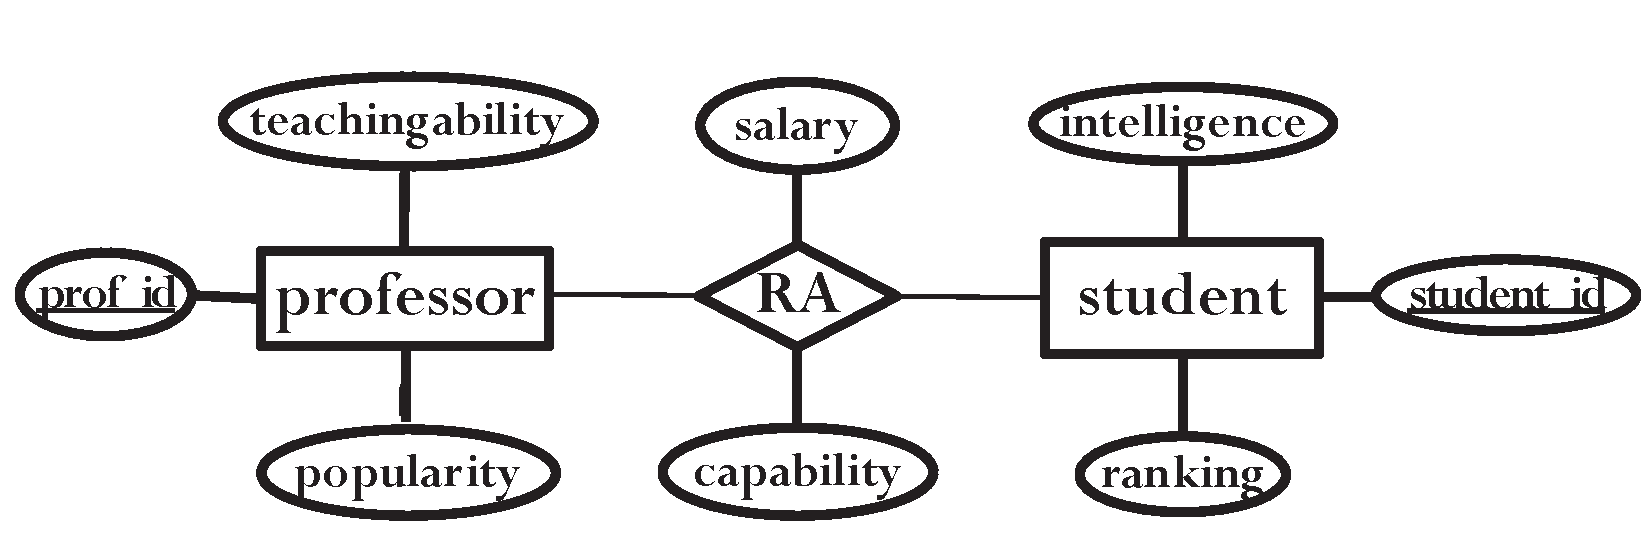
\includegraphics{university-schema.pdf} 
 } 
\caption{A relational ER Design for a university domain.}
 \label{fig:university-schema}
\end{figure}
\begin{figure}[htbp] %  figure placement: here, top, bottom, or page
 \centering
\resizebox{0.5\textwidth}{!}{
 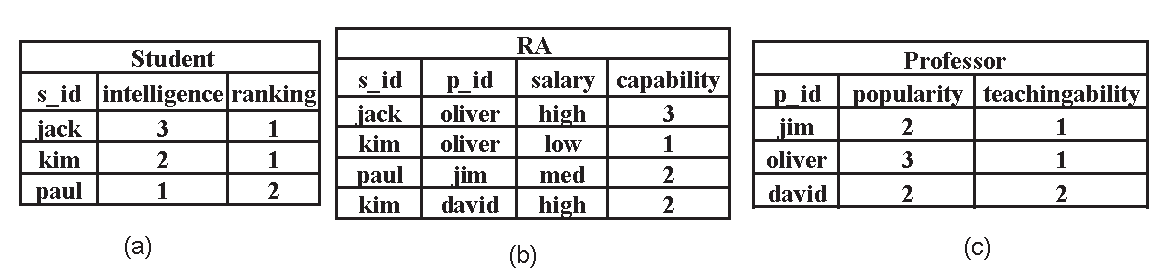
\includegraphics[width=0.5\textwidth]{university-tables.pdf} 
} 
%\caption{Database Table Instances: (a) $\student$, (b) $\course$, (c) $\prof$, (d) $\ra$, (e) $\reg$. }
\caption{Database Table Instances: (a) $\student$, (b) $\ra$, (c) $\prof$. }
 \label{fig:instance}
\end{figure}
\begin{figure}[htbp] %  figure placement: here, top, bottom, or page
 \centering
\resizebox{0.4\textwidth}{!}{
 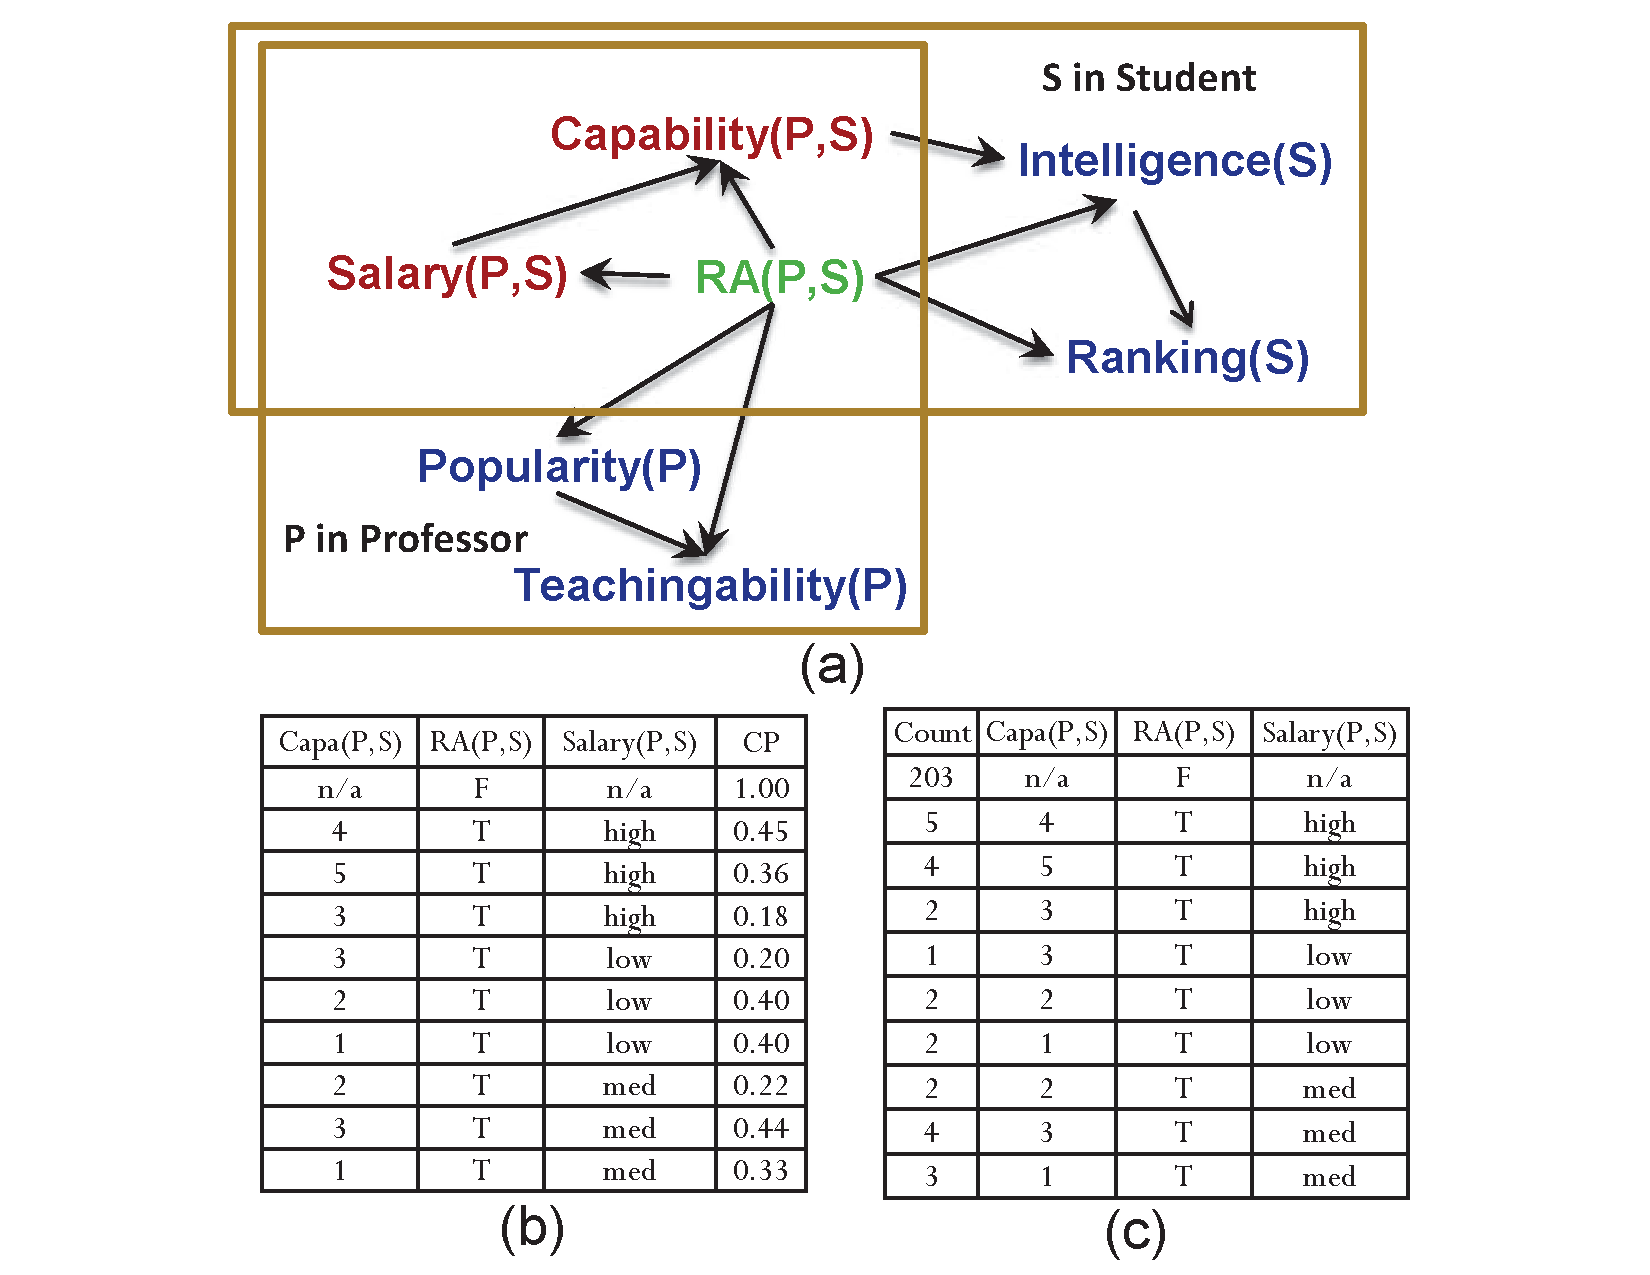
\includegraphics{pbn.pdf} 
} 
\caption{(a) Bayesian network for the University domain. We omit the $\it{Registered}$ relationship for simplicity. The network was learned from the University dataset \cite{bib:bbsite}.
(b) Conditional Probability table $Capability(\P,\S)\_\cptable$, for the node $Capability(\P,\S)$. Only value combinations that occur in the data are shown. This is an example of a factor table. (c) Contingency Table $Capability(\P,\S)\_\cttable$ for the node $Capability(\P,\S)$ and its parents. Both CP and CT tables are stored in an RDBMS.}
% \textbf{Zhensong: must be consistent about lower-case, upper case: which one?}
 \label{fig:pbn}
\label{fig:ct-cp-table}
\end{figure}

\subsection{Examples} \label{sec:examples} SRL has developed a number of formalisms for describing par-factors \cite{Kimmig2015}. 
%One option is to use SQL queries, as in Relational Markov networks \cite[Sec.3.2.1]{Kimmig2015}, another to use first-order logic (FOL) formulas, as in Markov Logic Networks \cite{Domingos2009}. 
%The model structure is a set of FOL formulas, and the parameters specify a weight for each. A grounding of an FOL formula with weight $w$ represents a value assignment to a ground set of par-RVs, with associated factor value $e^{w}$. 
First-order probabilistic graphical models
are popular both within SRL and the database community \cite{Kimmig2015,Wang2008}. The model structure is defined by edges connecting par-RVs. For instance, a \textbf{parametrized Bayesian network structure} is a directed acyclic graph whose nodes are par-RVs.  Figure \ref{fig:pbn} shows a Bayesian network for a University domain. We use the university example as a toy running example throughout the paper. The schema for the university domain is given in Figure~\ref{fig:university-schema}. This schema features only one relationship for simplicity; \FB\ learns a model for any number of relationships. While we describe \FB\ abstractly in terms of par-factors, for concreteness we illustrate it using Bayesian networks. The system takes as input a database instance like that shown in Figure~\ref{fig:instance}, and produces as output a graphical model like that shown in Figure~\ref{fig:pbn}.  


%For this instance, there are three possible ground random variables of the par-RV $\it{Popularity}(\P)$, namely $\it{Popularity}(\it{jim}), \it{Popularity}(\it{oliver}), \it{Popularity}(\it{david})$. 
A par-factor in a Bayesian network is associated with a \textbf{family} of nodes \cite[Sec.2.2.1]{Kimmig2015}. A family of nodes comprises a child node and all of its parents. For example, in the BN of Figure~\ref{fig:pbn}, one of the par-factors is associated with the par-RV set $\parrvs=\{\it{Capability}(\P,\S),\it{Salary}(\P,\S),\it{RA}(\P,\S)\}$. For the database instance of Figure~\ref{fig:instance}, there are $3\times3=9$ possible factors associated with this par-RV, corresponding to the Cartesian product of 3 professors and 3 students. The value of the factor $\phi$ is a function from an assignment of family node values to a non-negative real number. {\em In a Bayesian network, the factor value represents the conditional probability of the child node value given its parent node values.} These conditional probabilities are typically stored in a table as shown in Figure~\ref{fig:pbn}(b). This table represents therefore the function $\phi$ associated with the family par-factor. Assuming that all par-RVs have finite domains, a factor can always be represented by a \textbf{factor table} of the form Figure~\ref{fig:pbn}(b): there is a column for each par-RV in the factor, each row specifies a joint assignment of values to a par-RV, and the factor column gives the value of the factor for that assignment (cf. \cite[Sec.2.2.1]{Kimmig2015}).


%To evaluate a joint probability $P(\set{X}=\set{x})$ over all ground par-RVs using Equation~\ref{eq:parfactor}, we must count the number of times that each row in the CP-table is instantiated in the joint assignment $\set{X}=\set{x}$. 
The sufficient statistics for the $\it{Capability}(\P,\S)$ family can be represented in a contingency table as shown in Figure~\ref{fig:pbn}(c). For example, the first row of the contingency table indicates that the conjunction \\$\it{Capability}(\P,\S)=n/a,\it{Salary}(\P,\S)=n/a,\it{RA}(\P,\S) =\false$ is instantiated 203 times in the University database (publicly available at~\cite{bib:bbsite}). This means that for 203 professor-student pairs, the professor did not employ the student as an RA (and therefore the salary and capability of this RA relationship is undefined or $n/a$).

\subsection{SRL Structure Learning}

Algorithm~\ref{alg:learning} shows the generic format of a statistical-relational structure learning algorithm (adapted from 
\cite{Kimmig2015}%Kimming and Getoor
). The instantiation of procedures in lines 2, 3, 5 and 8 determines the exact behavior of a specific learning algorithm. The structure algorithm carries out a local search in the hypothesis space of graphical relational models. A set of candidates is generated based on the current model (line 3), typically using a search heuristic. For each candidate model, parameter values are estimated that maximize a model selection score function chosen by the  user (line 5). A model selection score is computed for each model given the parameter values, and the best-scoring candidate model is selected (line 7). 
We next discuss our system design and how it supports model discovery algorithms that follow the outline of Algorithm~\ref{alg:learning}. Figure~\ref{fig:architecture} outlines the system components and dependencies among them.

%\begin{algorithm}[htbp]
%%\label{Pivot_CT_Computation}
%
%\KwIn{Hypothesis space $ \mathcal H$ (describing graphical models), training data $\mathcal D$ (assignments to random variables), scoring function score ($\cdot$, $\mathcal D$)}
%\KwOut{A graph structure $G$ representing par-factors.}
%\begin{algorithmic}[1]
%\STATE $\mathcal G \leftarrow 	\emptyset$
%%$ $ h \leftarrow 	\emptyset ;$
%\WHILE{ \textsc{continue}($\mathcal G$, %$h$, 
%$\mathcal H$, score ($\cdot$, $\mathcal D$) )} 
%	\STATE{ $\mathcal R \leftarrow $ \textsc{refine}C\textsc{andidates}($\mathcal G, \mathcal H$)} 
% 	\FORALL{$R \in \mathcal R$} 
%		\STATE{$R \leftarrow$ \textsc{learn}P\textsc{arameters}($R$,score ($\cdot$, $\mathcal D$))} 
%    \ENDFOR
%	\STATE 	$\mathcal G \leftarrow$ argmax$_{G^{\prime} \in \mathcal R\cup \{G\}}$ score($G^{\prime} $, $\mathcal D$)
%%
%%	$h \leftarrow$ arg max$_{h^{\prime} \in \mathcal R\cup \{h\}}$ score($h^{\prime} $, $\mathcal D$)
%%	\STATE $\mathcal G \leftarrow \textsc{select}$($ \mathcal R$, score ($\cdot$, $\mathcal D$))
%\ENDWHILE
%
%%\COMMENT{Implements the algebra Equation~\ref{update} in proposition~\ref{PivotCT}.}
%\STATE \Return $G$
%\end{algorithmic}
%\label{alg:learning}
%\caption{Structure learning algorithm 
%%(instantiation of procedures in lines 2, 3, 5 and 8 determines exact behavior) 
%}
%\end{algorithm}
%

\begin{algorithm}[htbp]
%\label{Pivot_CT_Computation}

\KwIn{Hypothesis space $ \mathcal H$ (describing graphical models), training data $\mathcal D$ (assignments to random variables), scoring function score ($\cdot$, $\mathcal D$)}
\KwOut{A graph structure $G$ representing par-factors.}
\begin{algorithmic}[1]
\STATE $G \leftarrow 	\emptyset$
%$ $ h \leftarrow 	\emptyset ;$
\WHILE{ \textsc{continue}($G$, %$h$, 
$\mathcal H$, score ($\cdot$, $\mathcal D$) )} 
	\STATE{ $\mathcal R \leftarrow $ \textsc{refine}C\textsc{andidates}($G, \mathcal H$)} 
 	\FORALL{$R \in \mathcal R$} 
		\STATE{$R \leftarrow$ \textsc{learn}P\textsc{arameters}($R$,score ($\cdot$, $\mathcal D$))} 
    \ENDFOR
	\STATE 	$G \leftarrow$ argmax$_{G^{\prime} \in \mathcal R\cup \{G\}}$ score($G^{\prime} $, $\mathcal D$)
%
%	$h \leftarrow$ arg max$_{h^{\prime} \in \mathcal R\cup \{h\}}$ score($h^{\prime} $, $\mathcal D$)
%	\STATE $G \leftarrow \textsc{select}$($ \mathcal R$, score ($\cdot$, $\mathcal D$))
\ENDWHILE

%\COMMENT{Implements the algebra Equation~\ref{update} in proposition~\ref{PivotCT}.}
\STATE \Return $G$
\end{algorithmic}
\label{alg:learning}
\caption{Structure learning algorithm 
%(instantiation of procedures in lines 2, 3, 5 and 8 determines exact behavior) 
}
\end{algorithm}

%
\begin{figure*}[t]
\begin{center}
\resizebox{1\textwidth}{!}{
\includegraphics
%[width=0.8\textwidth]
{pipeline}
}
\caption{System Flow. All statistical objects are stored as first-class citizens in a DBMS. Objects on the left of an arrow are utilized for constructing objects on the right. Statistical objects are constructed and managed by different modules, shown as boxes. 
%[counts -> contingency table]
%Here the $DB$ denotes the original database, $DB\_RV$ denotes the database storing all random variables, 
%$DB\_CT$ denotes the database containing all the contingency tables  and $DB\_BN$ storing all the learned Bayes Nets.
\label{fig:architecture}}
\end{center}
\end{figure*}



\section{The Random Variable Database} 

Statistical-relational learning requires various metadata about the par-RVs in the model. These include the following. 

\begin{LaTeXdescription}
\item[Domain] the set of possible values of the par-RV.
\item[Types] Pointers to the first-order variables
in the par-RV. 
\item[Data Link] Pointers to the table and/or column in the input database associated with the par-RV. 
\end{LaTeXdescription}

%(1) {\em Domain}:  (2) {\em Types}: (3) For example, it is important that the par-RV $\it{Intelligence}(\S)$ and the par-RV $\it{RA}(\P,\S)$ both share the variable $\S$ and that this variable refers to entries in the $\it{Student}$ table. 
The metadata must be machine-readable. Following the in-database design philosophy, we store the metadata in tables so that an SRL algorithm can query it using SQL. The schema analyzer uses an SQL script that queries key constraints in the system catalog database and {\em automatically} converts them into metadata stored in the random variable database $VDB$. In contrast, existing SRL systems require users to specify information about par-RVs and associated types. 
Thus \FB\  utilizes the data description resources of SQL to facilitate the ``setup task'' for relational learning \cite{Walker2010}. Due to space constraints, we do not go into the details of the schema analyzer. Instead, we illustrate the general principles with the ER diagram of the University domain (Figure~\ref{fig:university-schema}). The Appendix  provides a full description with MySQL script. 

The translation of an ER diagram into a set of functors converts each element of the diagram into a functor, except for entity sets and key fields~\cite{Heckerman+al:SRL07}. Table~\ref{table:translation} illustrates this translation. In terms of database tables, attribute par-RVs correspond to {\em columns}. Relationship par-RVs correspond to {\em tables}, not columns. Including a relationship par-RV in a statistical model allows the model to represent uncertainty about whether or not a relationship exists between two entities~\cite{Kimmig2015}. The values of descriptive attributes of relationships are undefined for entities that are not related. We represent this by introducing a new constant $\it{n/a}$ in the domain of a relationship attribute~\cite{Milch2005}; see Figure~\ref{fig:attributes} (right). Table~\ref{table:vdb-schema} shows the schema for some of the tables that store metadata for 
each relationship par-RV, as follows. par-RV and FO-Var are custom types.

\begin{LaTeXdescription}
\item[Relationship] The associated input data table.
\item[Relationship\_Attributes] Descriptive attributes associated with the relationship and with the entities involved.
\item[Relationship\_FOVariables] The first-order variables contained in each relationship par-RV.\footnote{The schema assumes that all relationships are binary.}
\end{LaTeXdescription}

%There are different types of functors corresponding to the different types of ER diagram components. The simplest type represents an attribute of an entity set. 
%%We refer to such functors as \textbf{1Attributes}. 
%In Figure~\ref{fig:university-schema}, there are six entity attributes corresponding to attributes of Professors (2), Students (2), and Courses (2). 
%%The primary keys (p\_id, s\_id, c\_id) are identifiers that are not treated as random variables. 
%The metadata about these attributes can be stored in a database table as shown in Figure~\ref{fig:attributes}. 
%Relationship functors have the Boolean domain $\{\true,\false\}$.  There are two relationship sets in the diagram~\ref{fig:university-schema} corresponding to the $\it{Registered}$ and $\it{RA}$ relationships. A relationship set captures the information about which entities are related to each other in a certain way. For example, the database instance of Figure~\ref{fig:instance} represents that student Jack took course 101, and that student Kim did not take course 101.

%To relate a relationship par-RV to the original relationship data, we store pointers to the related entity sets as metadata. %We refer to attributes of relationships as \textbf{2Attributes}. 
%In Figure~\ref{fig:university-schema}, there are four relationship attributes, for Registered (2) and RA (2). 


\begin{table}[btp]
\caption{Translation from ER Diagram to Par-RVs}
 \centering
\resizebox{0.5\textwidth}{!}{
\begin{tabular}[c]{|l|l|l|}\hline
 ER Diagram &  Example &par-RV equivalent \\\hline
Entity Set  &Student, Course & $\S, \C$ \\\hline
 Relationship Set &RA & RA($\P$,$\S$) \\\hline
Entity Attributes  &intelligence, ranking & Intelligence($\S$), Ranking($\S$) \\\hline
Relationship Attributes  &capability, salary &Capability($\P, \S$), Salary($\P, \S$) \\\hline
\end{tabular}
}
 % end scalebox
 %\textbf{OS fix table}
 \label{table:translation}
\end{table}

%\begin{table}[hbtp]
%\caption{Selected Tables In the Variable Database Schema. Should add comments. Normally would have types too}
% \centering
%\resizebox{0.5\textwidth}{!}{
%\begin{tabular}{|r|r|r|r|r|r|}
%    \hline
%    \multicolumn{2}{|c|}{Table Name} & \multicolumn{4}{c|}{Column Names}  \\
%    \hline
%\multicolumn{2}{|l|}{Relationship\_1Variables} & \multicolumn{4}{l|}{\begin{tabular}{l}RVarID, 1VarID,   TABLE\_NAME, COLUMN\_NAME,  Pvid 
%\end{tabular} }  \\    \hline
%    \multicolumn{2}{|l|}{Relationship\_Pvariables} & \multicolumn{4}{l|}{\begin{tabular}{l}RVarID, Pvid,  TABLE\_NAME, COLUMN\_NAME,\\ REFERENCED\_COLUMN\_NAME \end{tabular}}  \\
%    \hline    
%%    \hline
%%    \multicolumn{2}{|l|}{Relationship\_2Variables } & \multicolumn{4}{l|}{\begin{tabular}{ll} RVarID, 2VarID\end{tabular}}  \\
%
%    \multicolumn{2}{|l|}{Relationship} & \multicolumn{4}{l|}{\begin{tabular}{lll}RVarID,  TABLE\_NAME, Pvid1,  Pvid2, \\ COLUMN\_NAME1,  COLUMN\_NAME2  \end{tabular}}  \\
%    \hline
%    \end{tabular}%
%}
% % end scalebox
% %\textbf{OS fix table}
% \label{table:vdb-schema}
%\end{table}



%\begin{table}[hbtp]
%\caption{Selected Tables In the Variable Database Schema.}
% \centering
%\begin{tabular}{|l|p{4cm}|p{1.5cm}|}
%\hline
% {Table Name}&  {Column Names} &{Comments} \\    \hline
%{Relationship\_Attributes}&  {RVarID: par-RV, AVarID: par-RV,  Pvid: FO-Var} &{links relationship par-RVs to associated descriptive attributes}  \\    \hline
%{Relationship\_Pvariables} & {RVarID: par-RV, Pvid: par-RV,  TABLE\_NAME: VARCHAR }& {?} \\    \hline    
%{Relationship} & {RVarID: par-RV,  TABLE\_NAME: VARCHAR, Pvid1: FO-Var, Pvid2: FO-Var } &{?}  \\ \hline
%    \end{tabular}%
% \label{table:vdb-schema}
%\end{table}


\begin{table}[hbtp]
\caption{Selected Tables In the Variable Database Schema.}
 \centering
\begin{tabular}{|l|p{6cm}|}
\hline
    {Table Name}&  {Column Names} \\\hline
{Relationship} & {RVarID: par-RV,  TABLE\_NAME: string} \\\hline
    {Relationship\_Attributes}&  {RVarID: par-RV, AVarID: par-RV,  FO-ID: FO-Var} \\\hline
    {Relationship\_FOvariables} & {RVarID: par-RV, FO-ID: FO-Var,  TABLE\_NAME: string}\\\hline
        \end{tabular}%
 \label{table:vdb-schema}
\end{table}


\begin{figure}[htbp] %  figure placement: here, top, bottom, or page
 \centering
\resizebox{0.4\textwidth}{!}{
 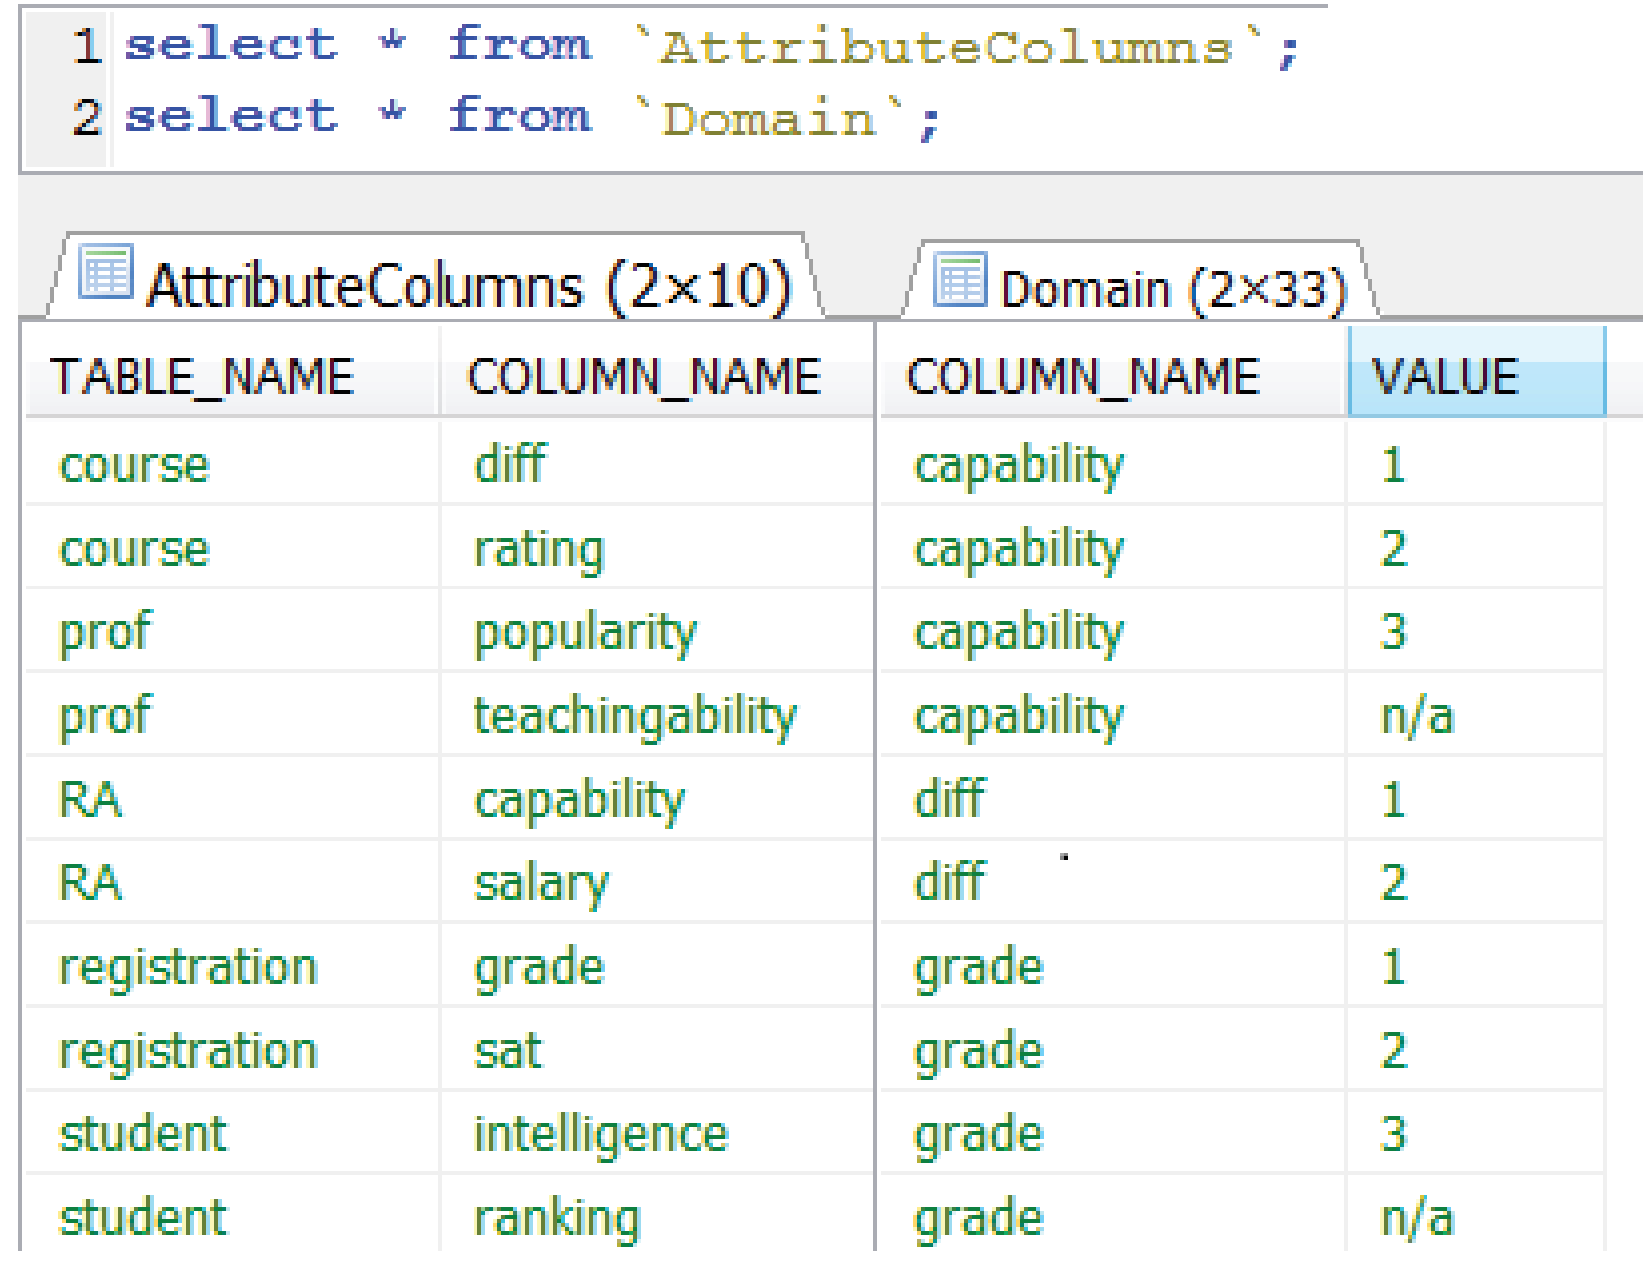
\includegraphics[width=0.5\textwidth]{attribute-domain.pdf} 
} 
\caption{ The metadata about attributes represented in \RVD database tables.  Left: The table $\it{AttributeColumns}$ specifies which tables and columns contain the functor values observed in the data. The column name is also the functor ID. Right: The table $\it{Domain}$ lists the domain for each functor.
}
 \label{fig:attributes}
\end{figure}

While we have described constructing the variable database for an ER model, different structured data models can be represented by an appropriate first-order logic vocabulary \cite{Kimmig2015}, that is, an appropriate choice of functors. For example, in a star schema, facts can be represented in the form $\functor(\dimension_{1},\ldots,\dimension_{k})$, where the first-order variable $\dimension_{i}$ ranges over the primary key of dimension table $i$. Attributes of dimension $i$ can be represented by a unary functor $\attribute(\dimension_{i})$. \FB can perform structure learning for different data models after the corresponding data format has been translated into the \RVD format.

%We refer to attributes of relationships as \textbf{2Attributes}. In Figure~\ref{fig:university-schema}, there are four 2Attributes corresponding to attributes of Registered (2) and RA (2). An important issue for relational data is that the values of descriptive attributes of relationships are undefined for entities that are not related. Following \cite{Russell2010}, we represent this by introducing a new constant $\it{n/a}$ in the domain of a 2Attribute; see Figure~\ref{fig:attributes} (right).
%
%Some complex patterns require more than one relationship variable for the same relationship functor. For instance, representing transitivity requires three relationship variables. The schema analyzer handles this by detecting self-relationships\cite{Heckerman+al:SRL07} and introducing additional relationship variables for them (cf. \cite{Schulte2012a}). 

%\paragraph{Discussion.} 

%
%
%Statistical analysis begins with a set of random variables. Formally, a \textbf{random variable} $\node$ is defined by a domain of possible values and a probability distribution over that domain. The more complex structure of multi-relational data leads to more complex structure for relational random variables, compared to random variables for single-table data.  
% In this section we discuss what types of random variables are suitable for analyzing relational databases; we refer to these as {\em relational random variables.} 
%%A major difference between single-table data and multi-relational data is that the latter has a more complex structure that represents heterogeneous classes of entities and multiple types of relationships. 
%Multi-relational learning requires making this structure explicit in machine-readable {\em metadata}. We discuss how to find and store relevant metadata about relational random variables. The metadata for a random variable must include the following at a minimum.
%(1) The domain of the random variable. For discrete random variables, this is a finite set of possible values.
%(2) Pointers to the table and/or column in the original database that contains the data relevant to the random variables. 
%
%%\begin{enumerate}
%%\item The domain of the random variable. For instance, a range of continuous values, or a finite set of discrete values.
%%\item Pointers to the table and/or column in the original database that contains the data relevant to the random variables. 
%%\end{enumerate}
%
%%There are various different notational systems for defining random variables in relational structures, of equivalent expressive power. 
%We adopt function-based notation from logic  \cite{Russell2010}. The expressive power of this formalism is equivalent to well-known logical query languages such as the domain relational calculus \cite{Ullman1982}. \FB\ can be adapted for other notational systems.
%
%\subsection{Relational Random Variables}
%A domain or \textbf{population} is a set of individuals.
%Individuals are denoted by lower case expressions (e.g., $\it{bob}$). 
%%A \textbf{first-order variable} is capitalized. 
%A \textbf{functor} represents a mapping
%$\functor: \population_{1},\ldots,\population_{a} \rightarrow \outdomain_{\functor}$
%where $\functor$ is the name of the functor, each $\population_{i}$ is a population, and $\outdomain_{\functor}$ is the output type or \textbf{range} of the functor. 
%In this paper we consider only functors with a finite range, disjoint from all populations.  If $\outdomain_{\functor} = \{\true,\false\}$, the functor $\functor$ is a (Boolean) \textbf{predicate}. A predicate with more than one argument is called a \textbf{relationship}; other functors are called \textbf{attributes}. We use uppercase for predicates and lowercase for other functors. Throughout this paper we assume that all relationships are binary, though this is not essential for our algorithm.
%%the populations associated with 
% %the variables are of the appropriate type for the functor.
%%
%A \textbf{Relational random variable} (RRV) is of the form $\functor(\X_{1},\ldots,\X_{a})$, where each $\X_{i}$ is a first-order variable \cite{Poole2003,Russell2010}. 
%Each first-order variable is associated with a population/type. In the context of RRVs, we therefore refer to first-order variables also as \textbf{logical variables}. An RRV has two components: A functor and a list of logical variables. We discuss first how the Schema Analzyer translates a relational database schema into a set of functors. Second, we describe a default method for combining logical variables with functors. 
%
%
%
%\subsection{Translating Entity-Relationship Models Into Functors}
% We assume a standard \textbf{relational schema} containing a set of tables, each with key fields, %typically
%descriptive attributes, and possibly foreign key pointers. 
%A \textbf{database instance} specifies the tuples contained in the tables of a given database schema. 
%We assume that tables in the relational schema can be divided into {\em entity tables} and {\em relationship tables} (ER model) \cite[Ch.2.2]{Ullman1982}.
%%This is the case whenever a relational schema is derived from an entity-relationship model  
% Figure~\ref{fig:university-schema} and Figure~\ref{fig:instance} show an ER diagram and an instance for a toy university domain, respectively. 
%%An ER diagram shows entity sets as boxes, relationships between entities as diamonds, and attributes as ovals.
%% Figure~\ref{fig:instance} shows a database instance for this ER diagram. 
%%An ER diagram for single-table data would contain just one entity set box with attributes, and no relationships. 
%
%
%
%%The functor formalism is rich enough to represent the constraints of an entity-relationship schema via the following translation: Entity sets correspond to populations, descriptive attributes to attribute functors, relationship tables to relationship functors, and foreign key constraints to type constraints on the arguments of relationship predicates. %, distinguishing attributes of entities ($\eatts$) and attributes of relationships ($\ratts$). 
%
%
%%\begin{table}[btp] \centering
%%\resizebox{0.4\textwidth}{!}{
%%\begin{tabular}[c]
%%{|l|c|l|l|}\hline
%% ER Design &Type & Functor &\RRV \\\hline
%%    \begin{tabular}{l}Entity \\Tables\end{tabular}&\begin{tabular}{l}Population \\Variables \end{tabular} & Student, Course & S, C \\\hline
%%    \begin{tabular}{l}Relation \\Tables \end{tabular}&RNodes &RA & RA(P,S) \\\hline
%%   \begin{tabular}{l}Entity \\Attributes \end{tabular}&1Nodes & intelligence, ranking &\begin{tabular}{l} \{intelligence(S), ranking(S)\}  \\=1Nodes(S) \end{tabular} \\\hline
%%  \begin{tabular}{l} Relationship \\Attributes \end{tabular}&2Nodes & teachingability, salary &\begin{tabular}{l}   \{teachingability(P,S), salary(P,S)\}  \\= 2Nodes(RA(P,S))\end{tabular}\\\hline
%%   
%%\end{tabular}
%%}
%% % end scalebox
%%\caption{Translation from ER Diagram to Relational Random Variable. \textbf{OS fix table}
%% \label{table:translation}}
%%\end{table}

%, just as random variables in single-table data do. 


%This supports applications like link prediction, (e.g., predicting whether two users are friends, \cite{Liben-Nowell2007}), and multiple link analysis for finding correlations among relationships (e.g., if user $u$ performs a web search for item $i$, is it likely that $u$ watches a video about $i$ ?). 
%
%Managing relationships raises several new issues compared to managing single-table column-based variables. 
% RRV's are called \textbf{1Variables} if their functor is a 1Attribute, \textbf{2Variables} if it is a 2Attribute, and \textbf{RVariables} if it is a relationship.
%\cite{BLOG}, 
%$\it{capability(\P,\S)} = n/a $
%we indicate this by writing 
%%$\it{grade}(\s,\c) = n/a$ 
%$\it{capability(\P,\S)} = n/a $ for a reserved constant $\it{n/a}$. 
%The assertion $\it{capability(\P,\S)}$ = n/a is therefore equivalent to the assertion that $\ra(\P,\S) = \false$.

%\subsection{Generating Default Relational Random Variables}

%We use upper case for Boolean-valued variables with domain $\{\true,\false\}$, such as RVariables. We use
%lower case for other random variables. 

%\subsection{logical variables and SQL Implementation} \label{sec:pvariables}
%
%The Schema Analyzer combines logical variables with functors to obtain full RRVs. The random variable database specifies a set of logical variables. A logical variable refers to an entity set. With each logical variable, we store a pointer to the original entity set as metadata. For example, the $\it{S}$ logical variable is associated with the the $\it{Student}$ table in the original database. 
%%In the example of Figure~\ref{fig:university-schema}, the type/foreign key constraints on the functors determine which logical variables to add, as shown in Table~\ref{table:translation}. In this case adding logical variables to functors enhances readability but is redundant given the type information in the schema.
%
%If the database schema contains a self-relationship, 
%by default, the Schema Analyzer creates three RVariables and three logical variables for the self-relationship. A self-relationship relates two entities of the same type.
%Neville and Jensen provide evidence that self-relationships are very common, so it is important to accommodate them in a statistical model \cite{Neville2007}.
%%
%%Some relational schemas require more than one logical variable for the same entity set. 
%%This additional expressive power becomes important in the presence of {\em self-relationships} \cite{Heckerman+al:SRL07}. 
%%A self-relationship relates two entities of the same type.
%%%, when we need to introduce more than one relationship node for the relationship functor. 
%%For example, the Mondial database contains a self-relationship $\it{Borders}$ that relates two countries, as shown in the ER diagram Figure~\ref{fig:mondial-er}. As they lead to major conceptual differences between relational and single-table data, we discuss self-relationships in some detail. Neville and Jensen provide evidence that self-relationships are very common, so it is important to accommodate them in a statistical model \cite{Neville2007}. Self-relationships give rise to {\em relational autocorrelations,} where the attribute value of an entity depends probabilistically on the attribute value of related entities \cite{Neville2007}. 
%%Relational autocorrelations are analogous to temporal autocorrelations in time series analysis, where there is a correlation between the value of a quantity at one time and the value of the same quantity at another. An autocorrelation cannot be represented in a model that contains only one random variable referring to the quantity in question. For time series, a common solution is to introduce {\em two} distinct random variables  that refer to the same quantity, but at different times. For instance, we may have two random variables $\it{temperature}_{t}$ and $\it{temperature}_{t+1}$. Similarly, to represent a relational autocorrelation between the continents of two different countries, we may introduce two random variables $\it{continent}_{\C_{1}}$ and $\it{continent}_{\C_{2}}$. The index notation can equivalently be replaced by function notation, writing $\it{continent}(\C_{1})$ and $\it{continent}(\C_{2})$ \cite{Milch2005}. 
%%%This leads to the concept of a relational random variable as previously defined. 
%%%
%%%In the ER diagram, there are two lines from the $\it{Countries}$ entity set to the $\it{Borders}$ relationship set 
%%%The ring structure may be represented with two different logical variables that each refer to the $\it{Countries}$ entity set. 
%%The corresponding relationship random variable is $\it{Borders}(\C_{1},\C_{2})$. The different positions of the 1st-order variables can represent different roles in the relationship. A random variable for a descriptive 2Attribute can also be represented using logical variables, for instance $\it{Border\_Length}(\C_{1},\C_{2})$. %\textbf{OS: add ER diagram for this simple Mondial example}. 
%%This notation is expressive enough to represent autocorrelations. 
%%For instance, the association rule
%%
%%\begin{small}
%%$\it{continent}(\C_{1}) = \it{Europe}, \it{Borders}(\C_{1}, \C_{2}) = \true \rightarrow \\\it{continent}(\C_{2}) = \it{Europe}$
%%\end{small}
%%
%%expresses that if two countries are neighbors and one is in Europe, the other country is likely to be in Europe. 
%%
%%Some complex patterns require more than one relationship variable for the same relationship functor. For instance, representing transitivity requires three relationship variables.
%%%as in 
%%%$$\it{Borders}(\C_{1}, \C_{2}) = \true,  \it{Borders}(\C_{1}, \C_{3}) = \true \rightarrow \it{Borders}(\C_{1}, \C_{3}) = \true.$$
%%%Since we introduce two logical variables referring to the same entity set, we need to duplicate the 1Nodes for that entity set. 
%%%This allows the logical language to represent that attributes of neighboring countries influence each other, 
%%%%Using a second relationship node with the $\it{Borders}$ functor allows us to represent such influences, 
%%%for instance in the following rule
%%%$$\it{continent}(\C_{1}) = \it{Europe}, \it{Borders}(\C_{1}, \C_{2}) = \true \rightarrow \it{continent}(\C_{2}).$$
%%If the database schema contains a self-relationship, 
%%by default, the Schema Analyzer creates three RVariables and three logical variables for the self-relationship.
%%%, together with the applicable 1Variables.
%%% (e.g., $\it{continent}(\C_{3}$).
%%It adds one logical variable for each role in the relationship. For each logical variable there is a separate set of corresponding 1Variables. In the Mondial example, there are two 1Variables $\it{continent}(\C_{1})$ and $\it{continent}(\C_{2})$.
%%\begin{figure}[htbp] %  figure placement: here, top, bottom, or page
%% \centering
%%\resizebox{0.4\textwidth}{!}{
%% 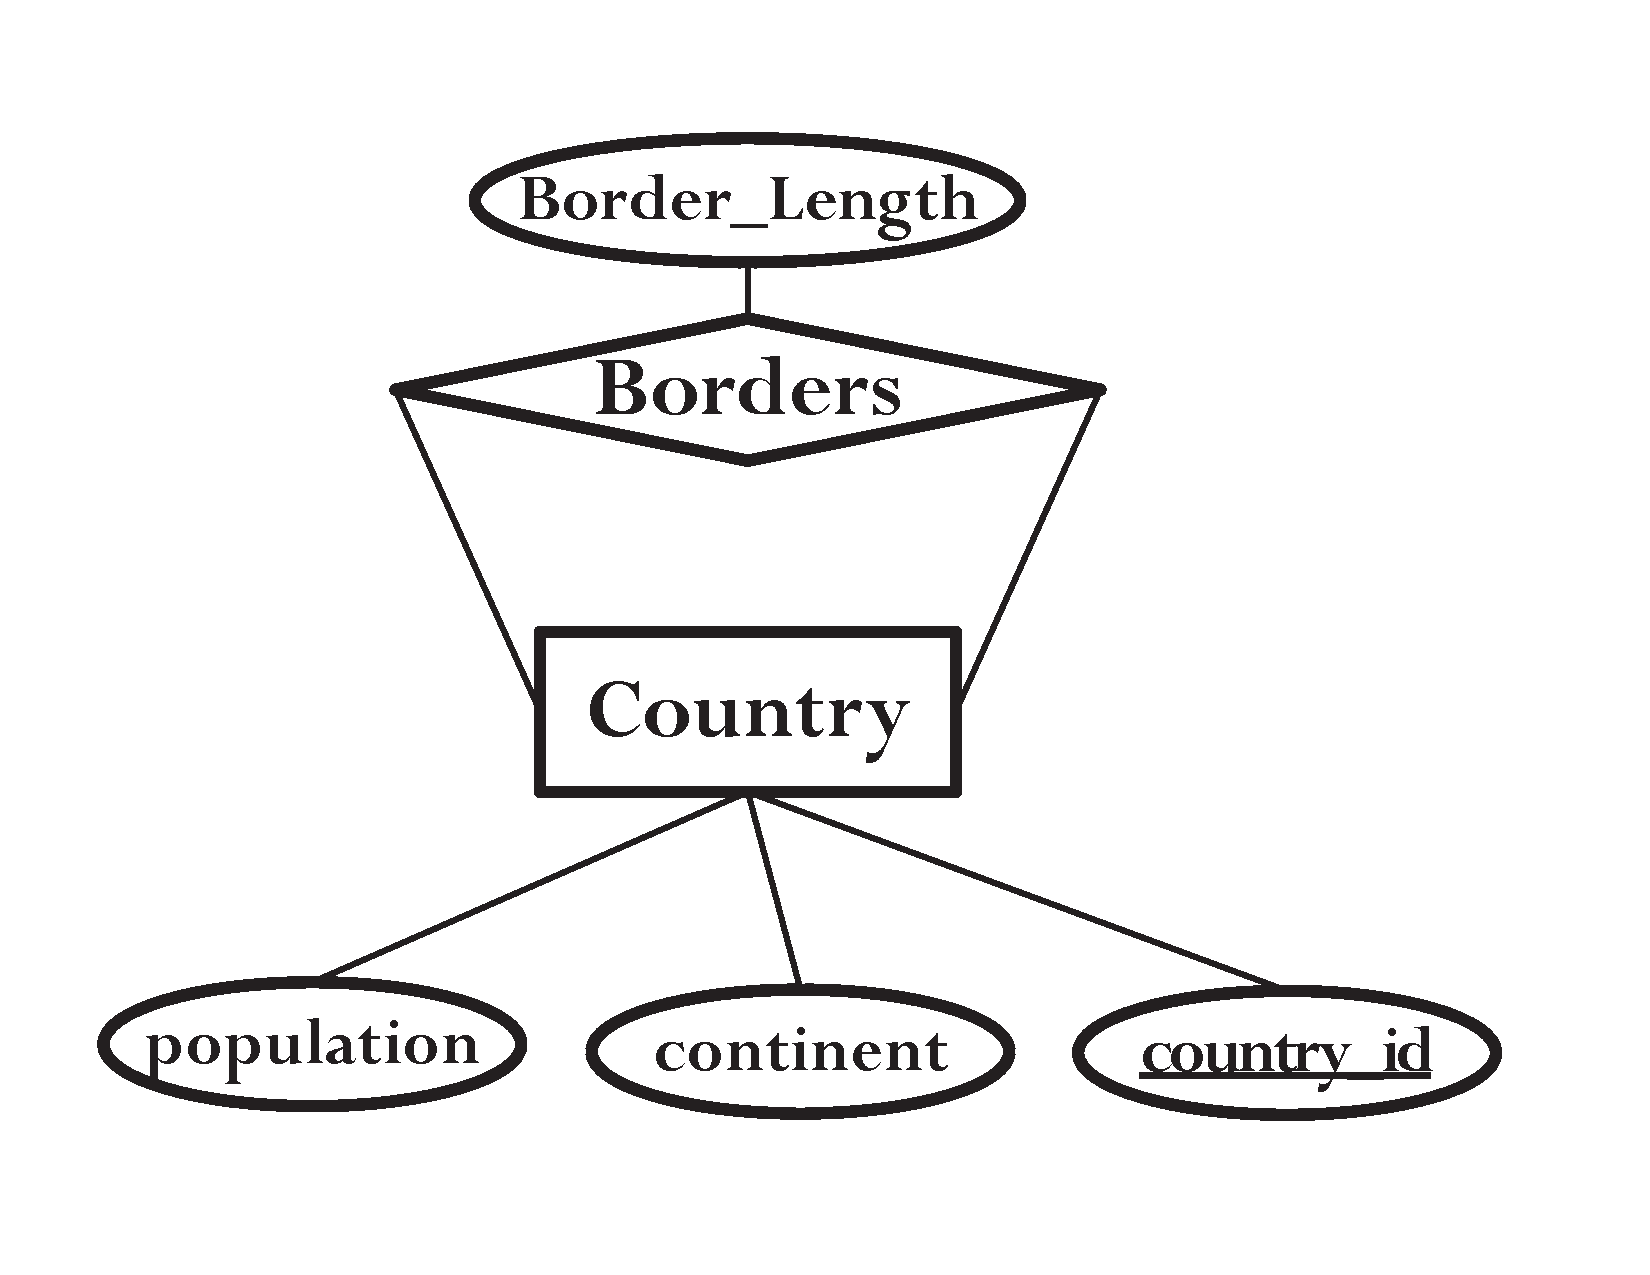
\includegraphics[width=0.4\textwidth]{mondial-er.pdf} 
%%} 
%%\caption{The ER diagram for Mondial database. $\it{Borders}$ is a self-relationship. 
%%}
%% \label{fig:mondial-er}
%%\end{figure}
%
%%\subsection{SQL Implementation}
%The metadata about the random variables is stored in the \textbf{random variable database} ($\RVD$). The relational schema of the $\RVD$ is shown in Figure~\ref{fig:rv_db}. %\textbf{OS: make 6 relations}. 
%The relational schema of the original database is represented in tables in the database system catalog. Given that both the system catalog and the $\RVD$ are databases, we can use SQL to transfer information from one to the other. %\textbf{OS make SQL query} 
%We show some of the SQL queries in the Schema Analzyer that the metadata about 1Attributes from the system catalog in our  university example. The full SQL script, 
%%included in the appendix, 
%also constructs tables for 2Attributes and relationship variables, and recognizes self-relationships by using foreign key pointer information. Figure~\ref{fig:rv_db} shows tables that are constructed by the SQL queries in the Schema Analyzer.
%%The full script is included in the supplementary material. 
%
%The first SQL query shows the construction of logical variables in our university example. 
%%It assume the existence of a KeyColumns table that contains triples (TableName, ColumnName, ConstraintName) to record which column in which table is associated with a key constraint. 
%%The query uses this information to identify tables with just one primary key column, which represent entity sets. 
%%The name of such tables is concatenated with an index to produce indexed logical variables as discussed in Section~\ref{sec:pvariables}. 
%The second query constructs a table listing 1Variables, which are relational random variables representing 1Attributes, identified by a 1Attribute name and a logical variable. 
%The use of the natural join operation to combine functors with logical variables illustrates how relational algebra elegantly supports defining new statistical objects from existing statistical objects.
%%After the random variable database has been created from the system catalog, the user  can add or substract relational random variables depending on the statistical patterns of interest.  such as WinBugs or mode declarations in Aleph.
%%As we discuss next, the remaining components of \FB\ depend only on the metadata in the $\RVD$ database, not on the system catalog.
%\begin{alltt}
%CREATE TABLE PVariables AS  SELECT 
%CONCAT(EntityTables.TABLE_NAME, `0') AS pvid,
%EntityTables.TABLE_NAME FROM
%(SELECT distinct TABLE_NAME, COLUMN_NAME 
%FROM   KeyColumns T WHERE
%1 = (SELECT  COUNT(COLUMN_NAME)   
%FROM   KeyColumns T2  WHERE     
%T.TABLE_NAME = T2.TABLE_NAME
%AND CONSTRAINT_NAME = 'PRIMARY')) 
%as EntityTables 
%
%CREATE TABLE 1Variables AS
%SELECT CONCAT(`\`', COLUMN_NAME,
% `(', pvid, `)', `\`') AS 1VarID,
%COLUMN_NAME,   pvid  FROM    
%PVariables   NATURAL JOIN  AttributeColumns;
%\end{alltt}
%
%\begin{figure}[htbp]
%\begin{center}
%\resizebox{0.5\textwidth}{!}{
%%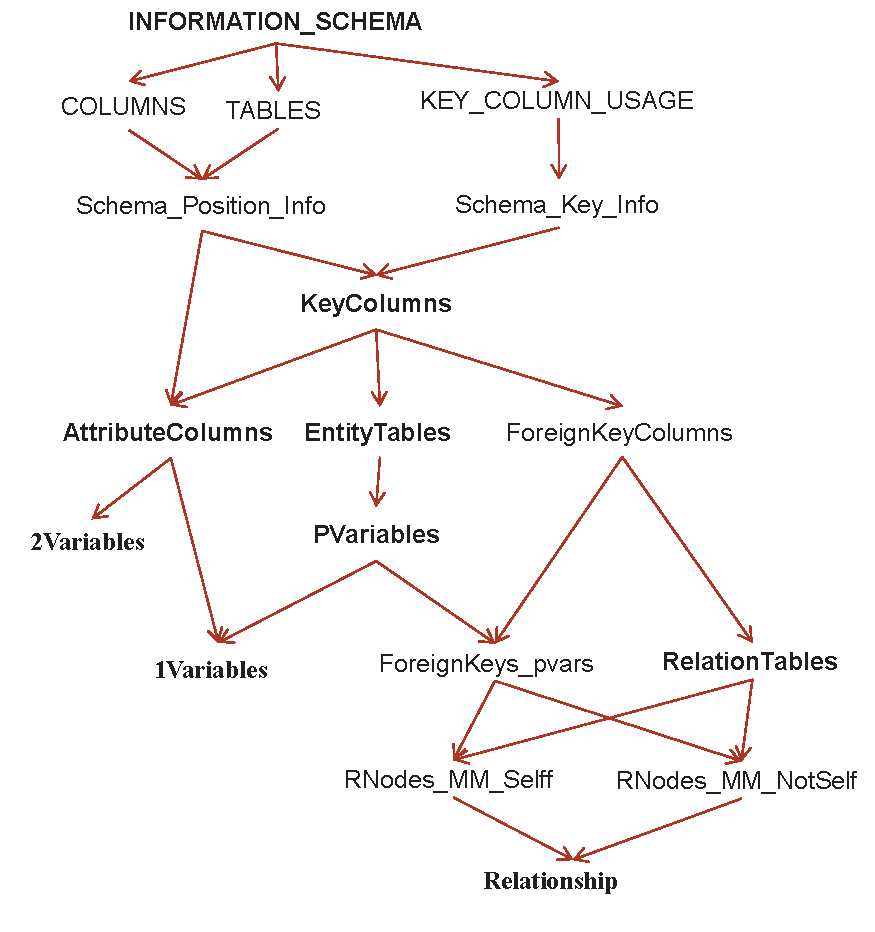
\includegraphics[width=0.5\textwidth]{rv_db.pdf} %move to the appendix
%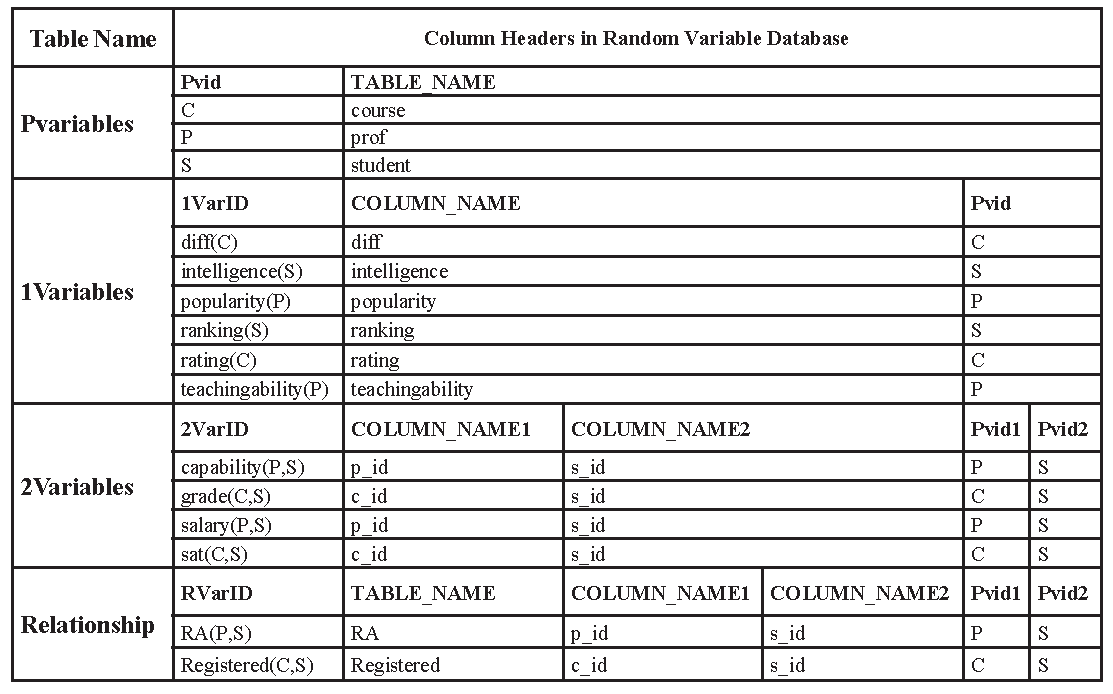
\includegraphics[width=0.5\textwidth]{rv_db_tables.pdf}
%}
%\caption{metadata: Main Tables in the Random Variable Database $\RVD$. 2Variables are relational random variables that represent attributes of binary relationships.
%\label{fig:rv_db}}
%\end{center}
%\end{figure}
%
%\section{The Count Manager} 
%A key service for machine learning that a data management system needs to provide is counting how many times a given pattern is instantiated in the data. Such counts are known as {\em sufficient statistics} \cite{Graefe1998}. 
%%Many statistical machine learning algorithms do not require full access to the original data, but only to sufficient statistics (hence the name ``sufficient''). So if a database management system is extended to provide sufficient statistics on demand, a learning algorithm for single-table data can be applied to relational database with few modifications. 
%%
%A novel aspect of \FB\ is managing sufficient statistics in the RDBMS, which has several important advantages. 
%%There are several reasons for employing an RDBMS for gathering sufficient statistics. 
%%(1). The machine learning application saves expensive data transfer by executing count operations in the database server space rather than local main memory. (2) SQL optimizations for aggregate functions such as SUM and COUNT can be leveraged. (3) Sufficient statistics can be computed once and stored/cached for future reuse in the RDBMS. For many datasets, the number of sufficient statistics runs in the millions and is too big for main memory \cite{Moore1998}.  
%%
%%An RDBMS provides disk storage and fast access for large numbers of sufficient statistics. 
%Previous work has exploited these advantages for single-table data \cite{Ordonez2010}. 
%We discuss how to compute sufficient statistics for a more general situation where sufficient statistics combine information {\em across} different tables in the relational database. In SQL terms, this requires combining aggregate functions with table joins. 
%
%
%\subsection{Relational Contingency Tables}
%%Our starting point is the observation that a statistical learning algorithm like a Bayes net learner does not require an enumeration of individuals tuples, but only {\em sufficient statistics} \cite{Heckerman1995,Schulte2011}. 
%%It is well-known in machine learning that a statistical learning algorithm like a Bayes net learner does not require an enumeration of individuals tuples, but only {\em sufficient statistics} \cite{Heckerman1995,Schulte2011}. 
%
% %A contingency table is defined as follows.
%%The Bayes net is learned from the contingency table. 
%
%%The count column in the $\ct$-table represents the number of instantiations for a given tuples of values in a row in the input database. 
%Sufficient statistics can be represented in {\em contingency tables} as follows \cite{Moore1998}. 
%Consider a fixed list of relational variables.
%%$\R_{1}, R_{2},\ldots,R_{m}$, and attribute nodes $\functor_{1},\ldots,\functor_{j}$. 
%A \textbf{query} is a set of $(variable = value)$ pairs where each value is of a valid type for the variable. 
%The \textbf{result set} of a query in a database $\D$ is the set of instantiations of the logical variables such that the query evaluates as true in $\D$.
%For example, in the database of Figure~\ref{fig:instance} the result set for the query 
%%$(\it{intelligence}(\S) = 2$, $\it{rank}(\S) = 1$, $\it{rating}(\C) = 3$, $\it{diff}(\C) = 1$, $\reg(\S,\C) = F)$
%$(\it{intelligence}(\S) = 2$, $\it{rank}(\S) = 1$, $\it{popularity}(\P) = 3$, $\it{teachingability}(\P) = 1$, $\ra(\P,\S) = T)$ 
%is the singleton $\{\langle \it{kim}, \it{Oliver}\rangle\}$. 
%% $\{\langle \it{kim}, \it{101}\rangle\}$
%The \textbf{count} of a query is the cardinality of its result set. 
%
%Every set of variables $\set{V} \equiv \{\V_{1},\ldots,\V_{n} \}$ has an associated \textbf{contingency table} ($\cttable$) denotes by $\cttable(\set{V})$. %$CT(\set{V})$. 
%This is a table with a row for each of the possible assignments of values to the variables in $\set{V}$, and a special integer column called $\qcount$. 
%The value of the $\qcount$ column in a row 
%corresponding to $V_{1} = v_{1},\ldots,V_{n} = v_{n}$ records the count of the 
%corresponding query. 
%Figure~\ref{fig:ct} shows the contingency table for the university database. The \textbf{contingency table problem} is to compute a contingency table for a target set of variables $\set{V} $ and a given database $\D$. 
%%Machine learning algorithms can leverage this capability in several different ways. A pre-counting approach computes a joint contingency table for all relational random variables at once \cite{Moore1998,Qian2014a}. Another possibility is to use postcounting \cite{lv2012}: Rather than precompute a large contingency table prior to learning, compute many small contingency tables for  small subsets of variables on demand during learning. I
%%n this paper, we describe an approach to compute contingency tables that leverages SQL capabilities. First, 
%\FB\ stores contingency tables as first-class database tables.
% %as in \cite{Qian2014a}. 
% The column headers of a contingency table are IDs for the relational random variables, plus an integer-valued count column. 
%
%%The value of a relationship attribute is undefined for entities that are not related.
%%Following \cite{Milch2005}, %\cite{BLOG}, 
%%%$\it{capability(\P,\S)} = n/a $
%%we indicate this by writing 
%%%$\it{grade}(\s,\c) = n/a$ 
%%$\it{capability(\P,\S)} = n/a $ for a reserved constant $\it{n/a}$. 
%%The assertion $\it{capability(\P,\S)}$ = n/a is therefore equivalent to the assertion that $\ra(\P,\S) = \false$.
%%For example, if student $\s$ is not registered in course $\c$, the value of $\it{grade}(\s,\c)$ is undefined. 
%
%
%\begin{figure}[htbp]
%\begin{center}
%\resizebox{0.5\textwidth}{!}{
%%%!%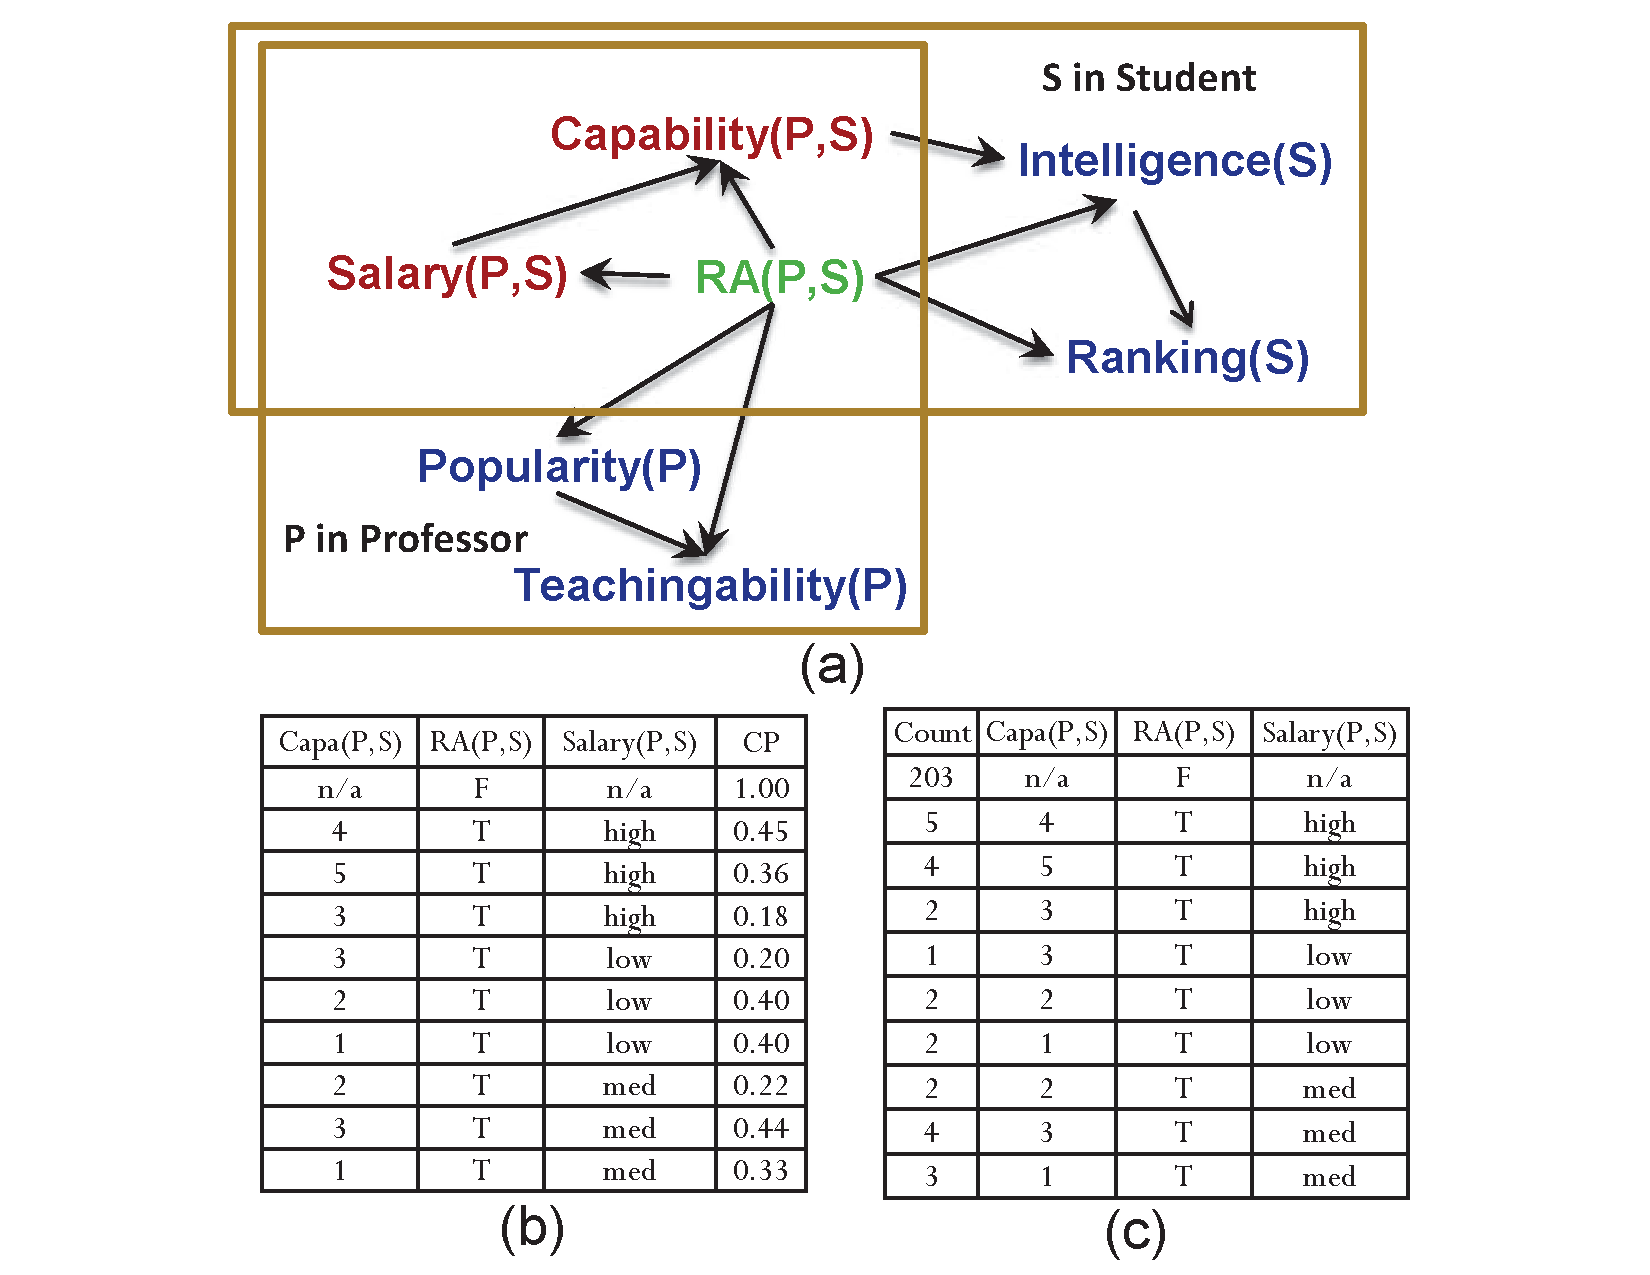
\includegraphics[width=1\textwidth]{pbn}
%%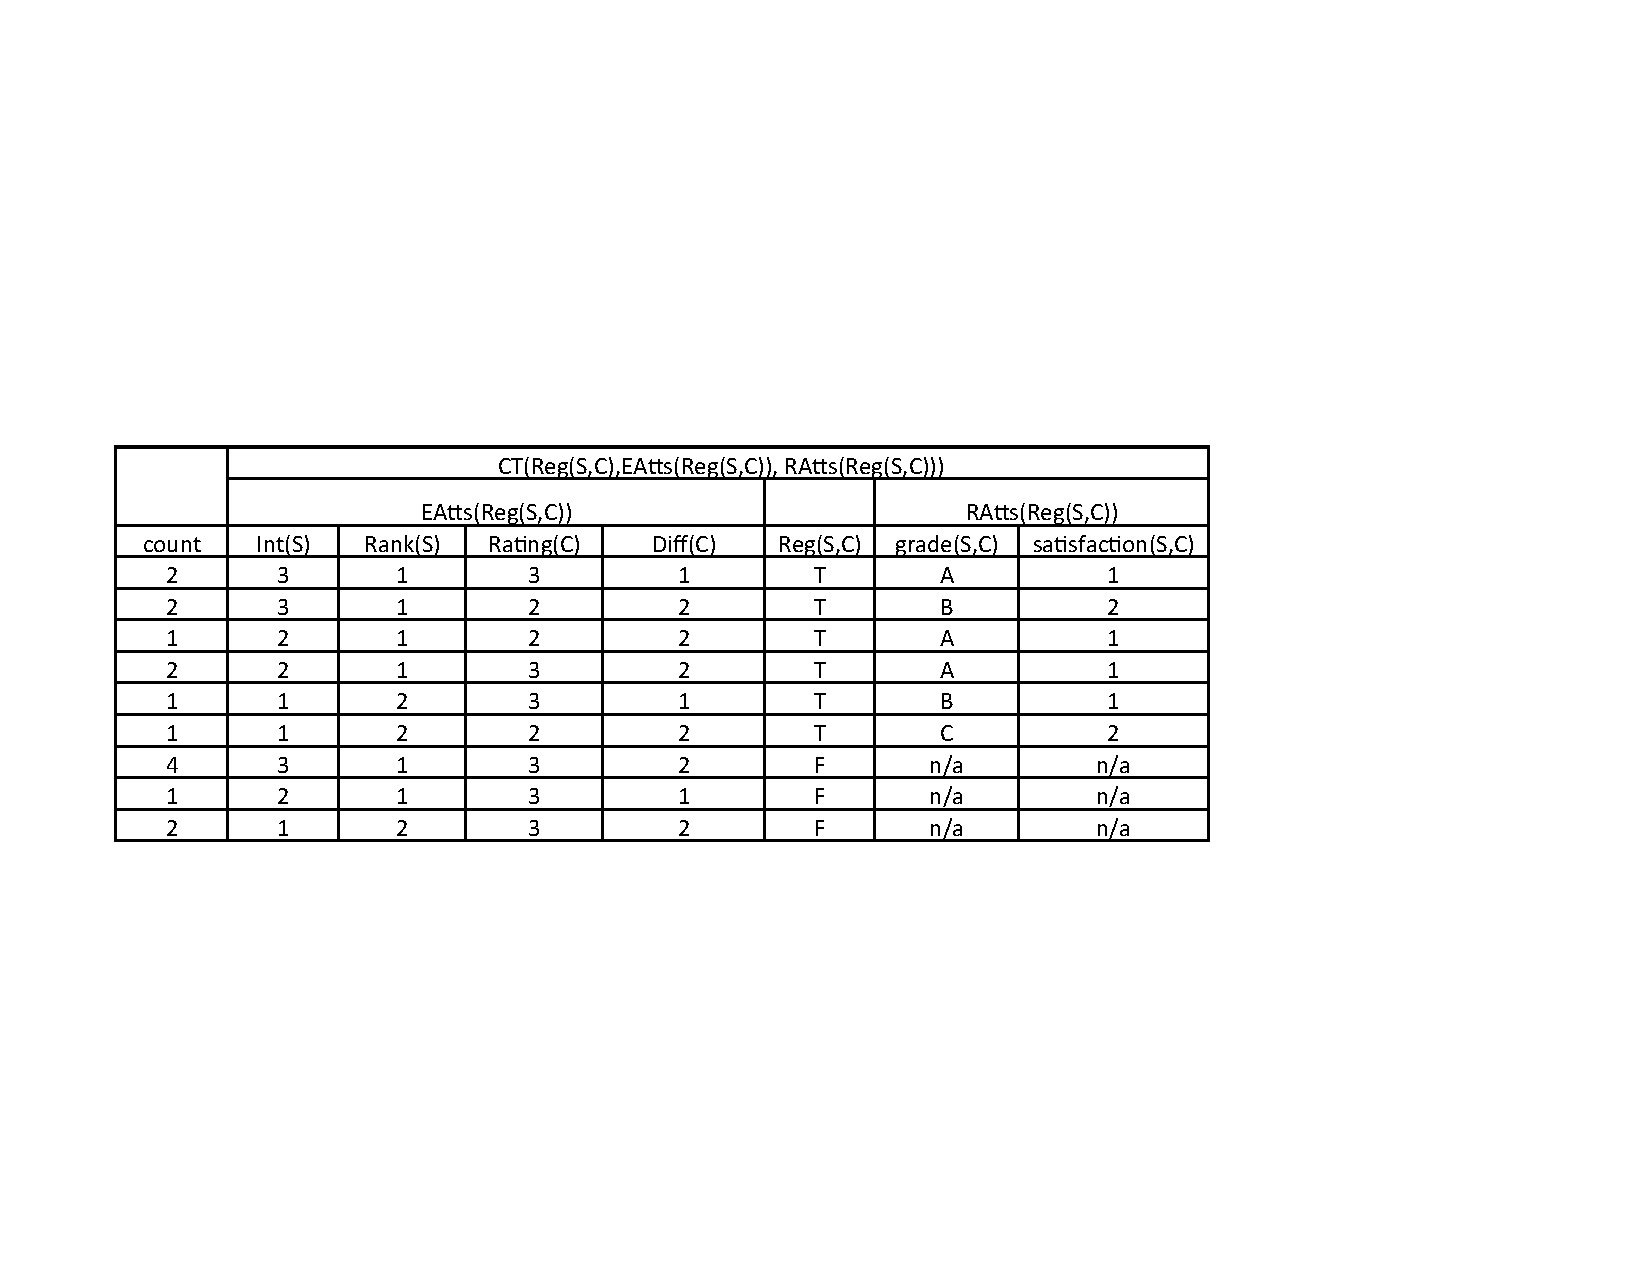
\includegraphics{figures/ct-table.pdf}
%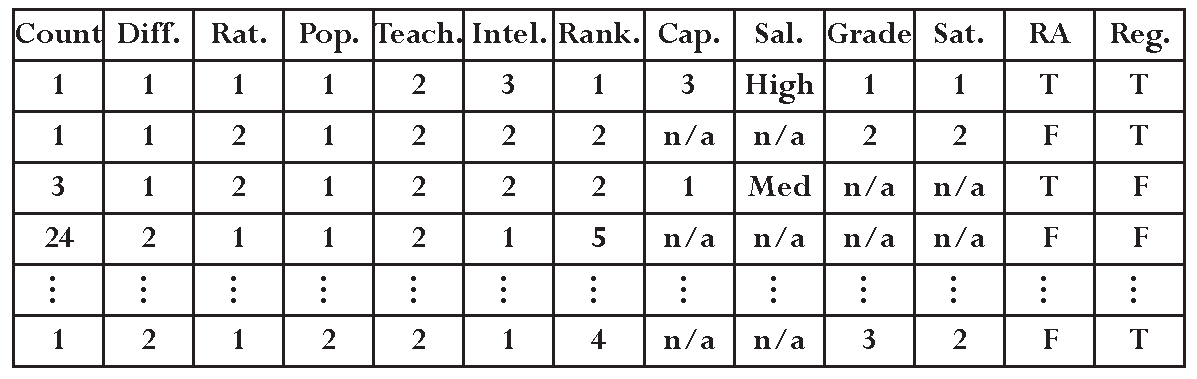
\includegraphics[width=0.5\textwidth]{uni-ct-table.pdf}
%}
%\caption{The contingency table for the university database. % for the attribute-relation table of Figure~\ref{fig:university-tables}
%Each row defines a query and its instantiation count in the database. For legibility, we show only functors, not the logical variables. %one possible assignment of such variables with its count. 
%% where for illustration we have added counts for another student like Jack and another course like 103.
%%use partial real table
%\label{fig:ct}}
%\end{center}
%\end{figure}
%
%%A \textbf{conditional contingency table}, written 
%%$$\ct(V_{1},\ldots,V_{k}|V_{k+1} = v_{k+1},\ldots, V_{k+m} = v_{k+m})$$
%%is the contingency table whose column headers are $V_{1},\ldots,V_{k}$ and whose counts are  defined by subset of instantiations that match the conditions to the right of the $\vert$ symbol.  %  \textbar 
%
%
%
%%To illustrate the SQL-based approach, we examine the following problem: precomputing a contingency table for all relational random variables that are associated with a given chain of relationships. A relationship chain is a list $$[\Relation_{1}(\argterms_{1}),\ldots,\Relation_{k}(\argterms_{k})]$$
%% of relationship variables such that each relationship variable shares at least one first-order variable with the preceding terms. In SQL terms, a relationship is formed by following foreign key pointers from one relationship table to the next. Sufficient statistics for relationship chains are important for discovering correlations between the attributes of entities that are related by paths of a certain type \cite{Getoor2007c} (called ``metapaths'' in \cite{Sun2012}). 
% 
%\subsection{Contingency Tables in SQL} The \textbf{Count Database} (CDB) stores a set of contingency tables each defined as a view. We describe how to create these views using SQL.  
%Each row in a $\cttable$ represents the count for a conjunctive query in a logical calculus; we refer to these as count-conjunction queries which 
%%It is well-known that conjunctive queries in a logical calculus 
%can be algorithmically translated into relational algebra queries and hence into an SQL query \cite{Ullman1982}.
%Our approach uses SQL itself to construct the count-conjunction query. We refer to this construction as an SQL \textbf{metaquery}. Metaqueries share the advantages of SQL over using a general programming language 
%%discussed in Section~\ref{sec:design}
%: They are compact, portable, and support automatic updates through the view mechanism.
%% (1) Succinctness and portability: Given the metadata in the random variable database, the metaquery is short, mainly requires a few natural joins. The metaquery requires only standard SQL, whereas a translation in an application language (e.g., Java) would have to be ported for each different application language. (2) Automatic Update: We can store the result of the metaquery as a database view. 
%% This means that changes in the original database schema are propagated to contingency tables. For instance, if a column $\it{gpa}$ is added to the $\it{Student}$ table in the original database schema, then the view definition adds this column automatically to contingency tables derived from the $\it{Student}$ table.

\section{The Count Manager} 

%\subsection{Relational Contingency Tables}
%Our starting point is the observation that a statistical learning algorithm like a Bayes net learner does not require an enumeration of individuals tuples, but only {\em sufficient statistics} \cite{Heckerman1995,Schulte2011}. 
%It is well-known in machine learning that a statistical learning algorithm like a Bayes net learner does not require an enumeration of individuals tuples, but only {\em sufficient statistics} \cite{Heckerman1995,Schulte2011}. 

 %A contingency table is defined as follows.
%The Bayes net is learned from the contingency table. 

%The count column in the $\ct$-table represents the number of instantiations for a given tuples of values in a row in the input database. 

The \textbf{count database} \CDB stores a set of  {\em contingency tables}. Contingency tables represent sufficient statistics as follows~\cite{Moore1998}. 
%~\cite{Qian2014a}. %\footnote{replace Moore by CIKM?}
Consider a fixed list of par-RVs.
%$\R_{1}, R_{2},\ldots,R_{m}$, and attribute nodes $\functor_{1},\ldots,\functor_{j}$. 
A \textbf{query} is a set of $(variable = value)$ pairs where each value is of a valid type for the variable. 
The \textbf{result set} of a query in a database $\D$ is the set of instantiations of the logical variables such that the query evaluates as true in $\D$.
For example, in the database of Figure~\ref{fig:instance} the result set for the query\\ 
%$(\it{intelligence}(\S) = 2$, $\it{rank}(\S) = 1$, $\it{rating}(\C) = 3$, $\it{diff}(\C) = 1$, $\reg(\S,\C) = F)$
$\it{RA}(\P,\S) = \true$, $\it{Capability}(\P,\S) = 3$, $\it{Salary}(\P,\S) = \it{high} $\\ is
the singleton $\{\langle \it{jack}, \it{oliver}\rangle\}$. 
% $\{\langle \it{kim}, \it{101}\rangle\}$
The \textbf{count} of a query is the cardinality of its result set. 

Every set of par-RVs $\set{V} \equiv \{\V_{1},\ldots,\V_{n} \}$ has an associated \textbf{contingency table} ($\cttable$) denoted by $\cttable(\set{V})$. %$CT(\set{V})$. 
This is a table with a row for each of the possible assignments of values to the variables in $\set{V}$, and a special integer column called $\qcount$. 
The value of the $\qcount$ column in a row 
corresponding to $V_{1} = v_{1},\ldots,V_{n} = v_{n}$ records the count of the 
corresponding query. 
Figure~\ref{fig:pbn}(b) shows a contingency table for the par-RVs $\it{RA}(\P,\S)$, $\it{Capability}(\P,\S)$, $\it{Salary}(\P,\S)$. The \textbf{contingency table problem} is to compute a contingency table for par-RVs $\set{V} $ and an input database $\D$. 
%Machine learning algorithms can leverage this capability in several different ways. A pre-counting approach computes a joint contingency table for all relational random variables at once \cite{Moore1998,Qian2014a}. Another possibility is to use postcounting \cite{lv2012}: Rather than precompute a large contingency table prior to learning, compute many small contingency tables for  small subsets of variables on demand during learning. I
%n this paper, we describe an approach to compute contingency tables that leverages SQL capabilities. First, 
%\FB\ stores contingency tables as first-class database tables.
 %as in \cite{Qian2014a}. 
 
%The value of a relationship attribute is undefined for entities that are not related.
%Following \cite{Milch2005}, %\cite{BLOG}, 
%%$\it{capability(\P,\S)} = n/a $
%we indicate this by writing 
%%$\it{grade}(\s,\c) = n/a$ 
%$\it{capability(\P,\S)} = n/a $ for a reserved constant $\it{n/a}$. 
%The assertion $\it{capability(\P,\S)}$ = n/a is therefore equivalent to the assertion that $\ra(\P,\S) = \false$.
%For example, if student $\s$ is not registered in course $\c$, the value of $\it{grade}(\s,\c)$ is undefined. 


%\begin{figure}[htbp]
%\begin{center}
%\resizebox{0.5\textwidth}{!}{
%%%!%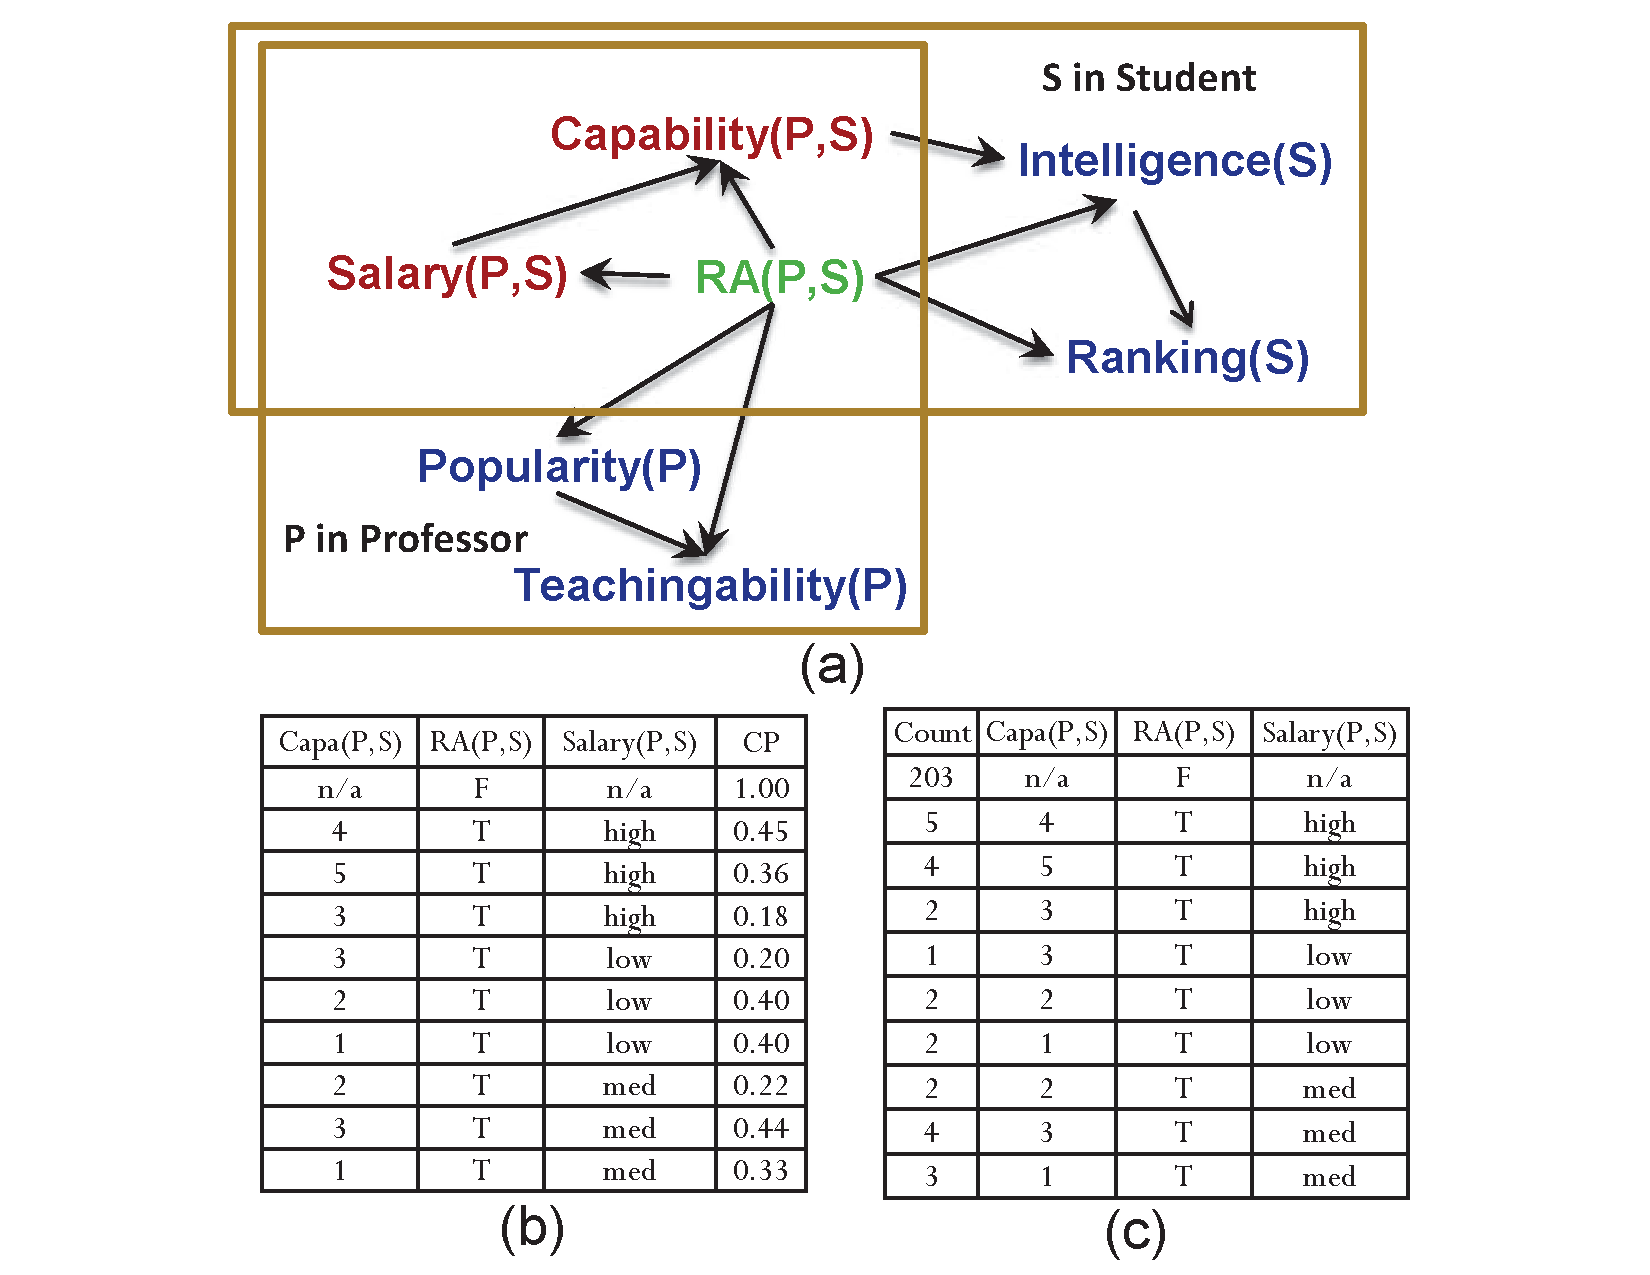
\includegraphics[width=1\textwidth]{pbn}
%%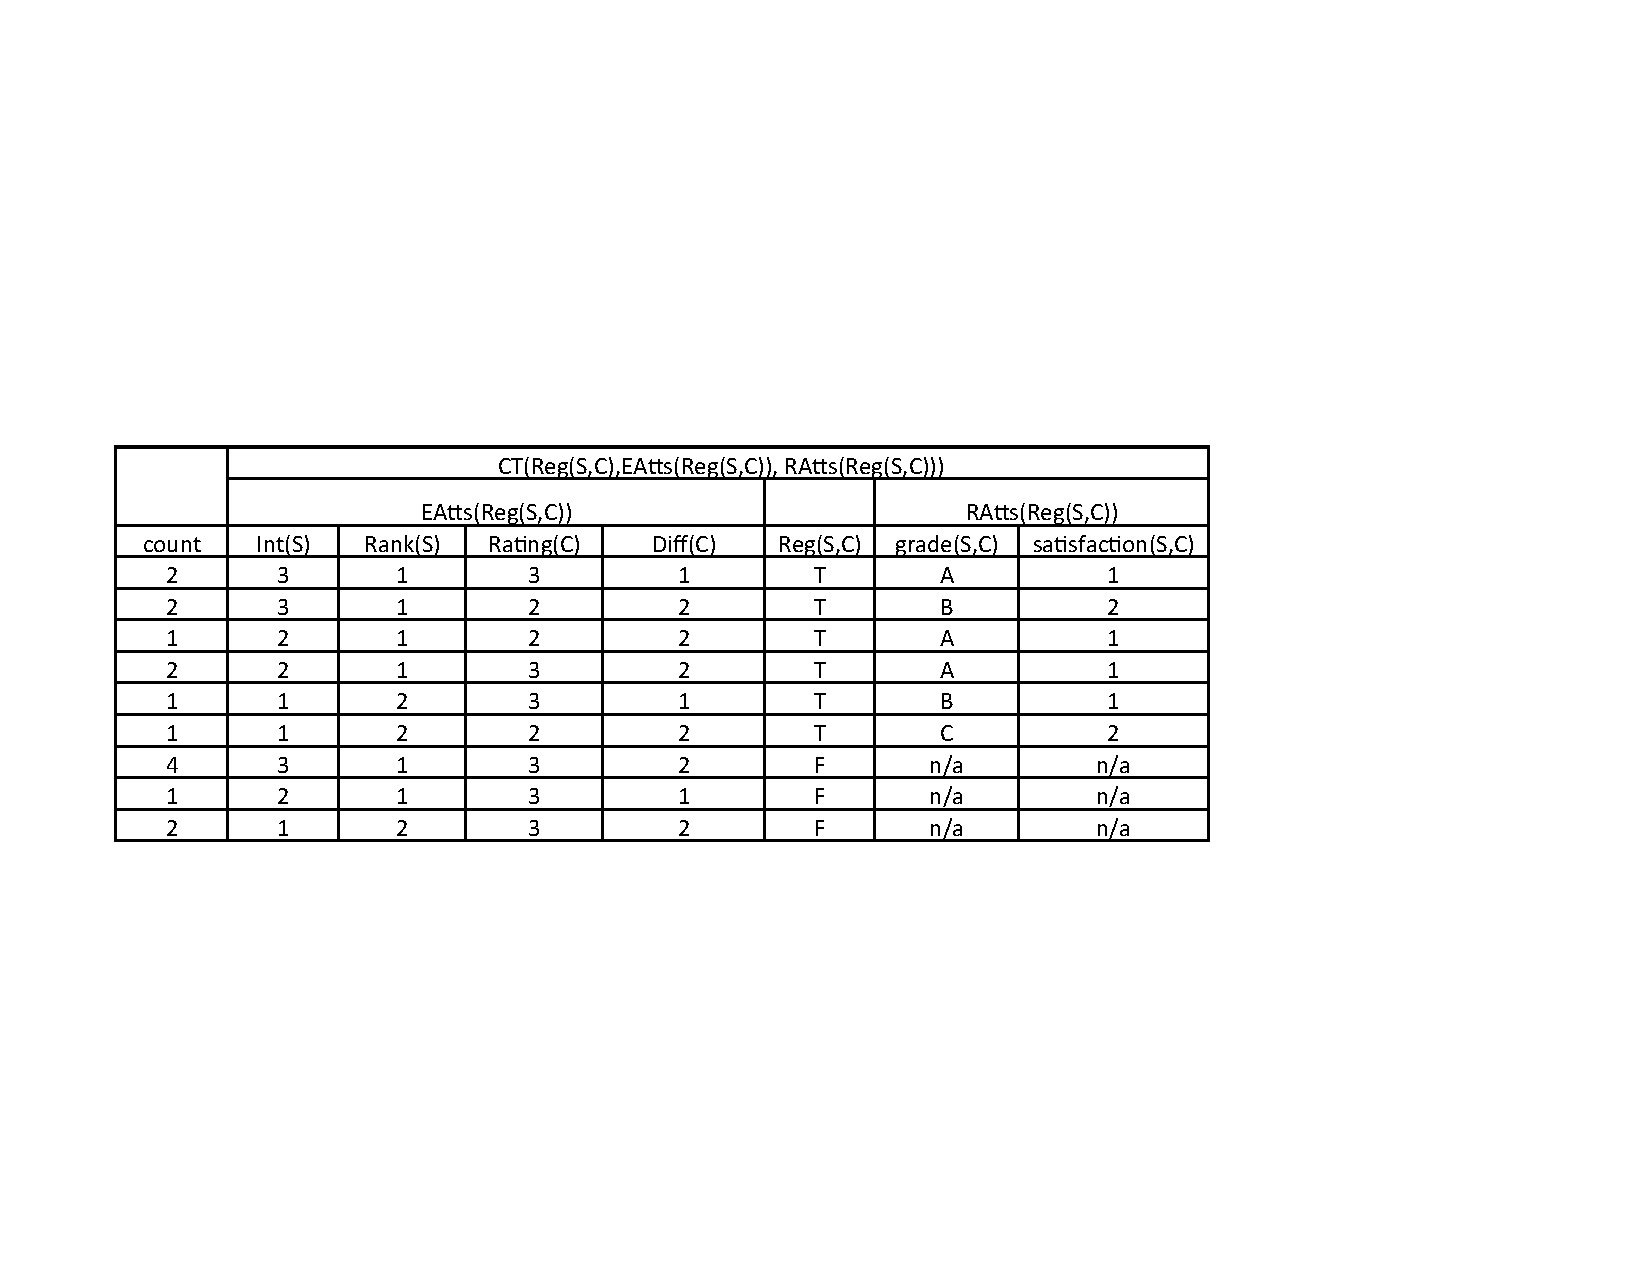
\includegraphics{figures/ct-table.pdf}
%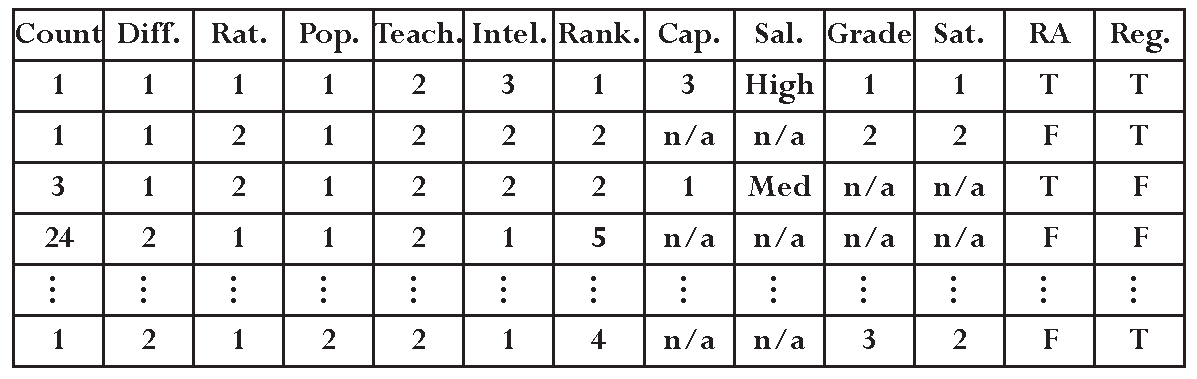
\includegraphics[width=0.5\textwidth]{uni-ct-table.pdf}
%}
%\caption{Part of the contingency table for the university database. % for the attribute-relation table of Figure~\ref{fig:university-tables}
%Each row defines a query and its instantiation count in the database. For legibility, we show only functors, not the logical variables. %one possible assignment of such variables with its count. 
%% where for illustration we have added counts for another student like Jack and another course like 103.
%%use partial real table
%\label{fig:ct}}
%\end{center}
%\end{figure}

%A \textbf{conditional contingency table}, written 
%$$\ct(V_{1},\ldots,V_{k}|V_{k+1} = v_{k+1},\ldots, V_{k+m} = v_{k+m})$$
%is the contingency table whose column headers are $V_{1},\ldots,V_{k}$ and whose counts are  defined by subset of instantiations that match the conditions to the right of the $\vert$ symbol.  %  \textbar 



%To illustrate the SQL-based approach, we examine the following problem: precomputing a contingency table for all relational random variables that are associated with a given chain of relationships. A relationship chain is a list $$[\Relation_{1}(\argterms_{1}),\ldots,\Relation_{k}(\argterms_{k})]$$
% of relationship variables such that each relationship variable shares at least one first-order variable with the preceding terms. In SQL terms, a relationship is formed by following foreign key pointers from one relationship table to the next. Sufficient statistics for relationship chains are important for discovering correlations between the attributes of entities that are related by paths of a certain type \cite{Getoor2007c} (called ``metapaths'' in \cite{Sun2012}). 
 
%\subsection{Metaqueries for Computing Contingency Tables With SQL} 
%The \textbf{Count Database} (CDB) stores a set of contingency tables, each defined as a view. 

{\em SQL Implementation With Metaqueries.}
We describe how the contingency table problem can be solved using SQL. % with {\em metaqueries}. 
This is relatively easy for a {\em fixed} set of par-RVs; the challenge is a general construction that works for different sets of par-RVs. For a fixed set, a  contingency table can be computed by an SQL count(*) query of the form 
%Each row in a $\cttable$ represents the count for a conjunctive query;
% %in a logical calculus; 
% we refer to these as \textbf{count-conjunction} queries.
%It is well-known that conjunctive queries in a logical calculus can be algorithmically translated into relational algebra queries and hence into an SQL query \cite{Ullman1982}. 
%
%Metaqueries share the advantages of SQL over using a general programming language discussed in Section~\ref{sec:design}: They are compact, portable, and support automatic updates through the view mechanism.
% (1) Succinctness and portability: Given the metadata in the random variable database, the metaquery is short, mainly requires a few natural joins. The metaquery requires only standard SQL, whereas a translation in an application language (e.g., Java) would have to be ported for each different application language. (2) Automatic Update: We can store the result of the metaquery as a database view. 
% This means that changes in the original database schema are propagated to contingency tables. For instance, if a column $\it{gpa}$ is added to the $\it{Student}$ table in the original database schema, then the view definition adds this column automatically to contingency tables derived from the $\it{Student}$ table.
%
%A contingency table for a set of random variables can be computed by an SQL count-conjunction query of the form 
\begin{alltt}
CREATE VIEW CT-table(<VARIABLE-LIST>) AS
SELECT COUNT(*) AS count, <VARIABLE-LIST>
FROM TABLE-LIST
GROUP BY VARIABLE-LIST
WHERE <Join-Conditions>
\end{alltt}
%As the top level of  Figure~\ref{fig:flow} illustrates, 
%The required counts involving only true relationships can be computed using the standard SQL constructs COUNT(*) and GROUP BY. 
%The general form of these operations is the same for every input database. 
%The varying part is the list of columns to be included, which depends on the input database. 
%For a fixed database, the column lists can be hard-coded. 
%To achieve a general solution when the column list is not known in advance, we introduce a new approach that we refer to as an SQL \textbf{metaquery}. 

%Thus an SQL metaquery maps schema information to the components of another SQL query. 
\FB\ uses SQL itself to construct the count-conjunction query. We refer to this construction as an SQL \textbf{metaquery}. We represent a count(*) query in 
four kinds of tables: the Select, From, Where and Group By tables. Each of these tables lists the entries in the corresponding count(*) query part.
%The Select table lists the entries in the Select clause of the target query, the From table lists the entries in the From clause, and similar for Where and Group By tables. 
%
Given the four metaquery tables, the corresponding SQL count(*) query can be easily constructed and executed in an application to construct the contingency table.
Given a list of par-RVs as input, the metaquery tables are constructed as follows
from the metadata in the database $\RVD$.  




\begin{LaTeXdescription}
\item[FROM LIST] Find the tables referenced by the \RRV's. A \RRV ~references the entity tables associated with its first-order variables (see VDB.Relationship\_FOvariables). Relational \RRV's also reference the associated relationship table (see VDB.Relationship). 
\item[WHERE LIST] Add join conditions on the matching primary keys of the referenced tables in the WHERE clause. The primary key columns are recorded in VDB. 
\item[SELECT LIST] For each attribute \RRV, find the corresponding column name in the original database (see VDB.AttributeColumns). Rename the column with the ID of the \RRV. Add a $\qcount$ column.
\item[GROUP BY LIST] The entries of the Group By table are the same as in the Select table without the $\qcount$ column.
\end{LaTeXdescription}

% The metaquery accesses tables in the Relational Random Variable Database. %We omit further details due to space constraints.

\begin{figure}[htb]
\begin{center}
\resizebox{0.45\textwidth}{!}{
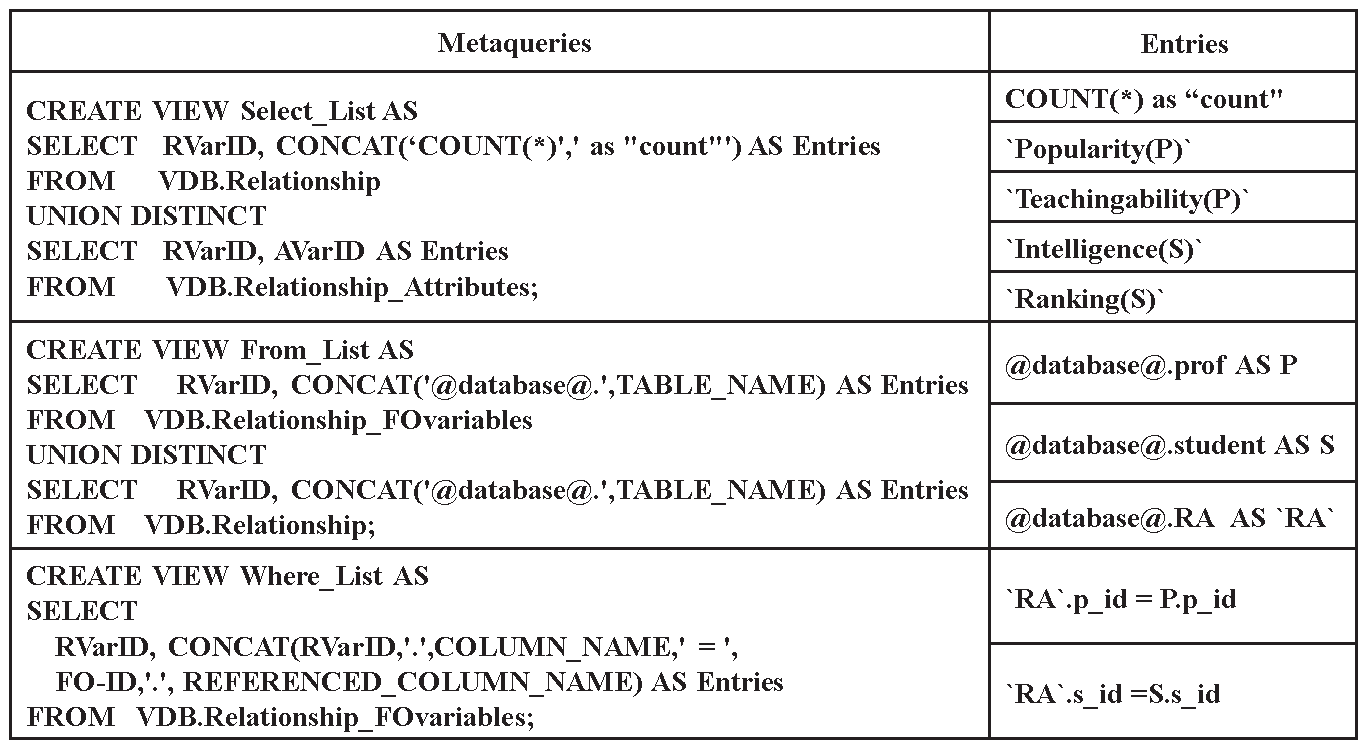
\includegraphics[width=0.45\textwidth]{meta-query.pdf}
}
\caption{Example of metaquery results based on university database and the par-RV metadata (Table \ref{table:vdb-schema}).
%\textbf{Zhensong: create views}
~\label{fig:meta-query}}
\end{center}
\end{figure}
%\begin{table}[htbp]  \caption{Schema for Random Variable Database (VDB)}
%  \centering
%\resizebox{0.5\textwidth}{!}{
%    \begin{tabular}{|r|r|r|r|r|r|}
%    \hline
%    \multicolumn{2}{|c|}{Table Name} & \multicolumn{4}{c|}{Schema}  \\
%    \hline
%\multicolumn{2}{|l|}{Relationship\_1Variables} & \multicolumn{4}{l|}{\begin{tabular}{l}RVarID, 1VarID,   TABLE\_NAME, COLUMN\_NAME,  Pvid 
%\end{tabular} }  \\    \hline
%    \multicolumn{2}{|l|}{Relationship\_Pvariables} & \multicolumn{4}{l|}{\begin{tabular}{l}RVarID, Pvid,  TABLE\_NAME, COLUMN\_NAME,\\ REFERENCED\_COLUMN\_NAME \end{tabular}}  \\
%    \hline    
%%    \hline
%%    \multicolumn{2}{|l|}{Relationship\_2Variables } & \multicolumn{4}{l|}{\begin{tabular}{ll} RVarID, 2VarID\end{tabular}}  \\
%
%    \multicolumn{2}{|l|}{Relationship} & \multicolumn{4}{l|}{\begin{tabular}{lll}RVarID,  TABLE\_NAME, Pvid1,  Pvid2, \\ COLUMN\_NAME1,  COLUMN\_NAME2  \end{tabular}}  \\
%    \hline
%    \end{tabular}%
%}
%
%  \label{table:rvdb1}%
%\end{table}%

Figure~\ref{fig:meta-query} shows an example of a metaquery for the university database. This metaquery defines a view that in turn defines a contingency table for the random variable list associated with the relationship table $\ra$. This list includes the entity attributes of professors and of students, as well as the relationship attributes of the $\ra$ relationship. 
The Bayesian network of Figure~\ref{fig:pbn} was learned from this contingency table. 
The  contingency table defined by the metaquery of Figure~\ref{fig:meta-query} contains only rows where the value of $\ra$ is true. The M\"obius Virtual Join~\cite{Qian2014a} can be used to extend this contingency table to include counts for when $\ra$ is false, like the table shown in Figure~\ref{fig:pbn}(c).

\section{The Model Manager}

The Model Manager provides two key services for statistical-relational structure learning: 1) Estimating and storing parameter values (line 5 of Algorithm~\ref{alg:learning}). 2) Computing one or more model selection scores (line 7 of Algorithm~\ref{alg:learning}).  \FB\ uses a {\em store+score} design for these services, which is illustrated in 
Figure~\ref{fig:learning}. 
%illustrates a {\em store+score} design that supports the generic structure learning process of Algorithm~\ref{alg:learning}.  
A \textbf{model structure table} represents a candidate model. When a candidate model structure is inserted, a view uses the sufficient statistics from a contingency table to compute a table of parameter values. Another view uses the parameter values and sufficient statistics together to compute the score for the candidate model. 
%In this store+score design, the RDBMS provides model selection scores as a service to the SRL client. 

\begin{figure}[htbp]
\begin{center}
\resizebox{0.4\textwidth}{!}{
\includegraphics
%[width=0.8\textwidth]
{learning}
}
\caption{Dependencies Among Key Components of the Model  Manager. 
\label{fig:learning}}
\end{center}
\end{figure}

\subsection{The \MDB Schema}

The relational schema for the Models Database is shown in Table~\ref{table:mdb-schema}. The @par-RVID@ parameter refers to the ID  of a par-RV, for instance $\it{Capability}(\P,\S)$.
The model manager stores a set of factor tables (cf. Section~\ref{sec:examples}). In a graphical model, each factor is defined by the local topology of the model template graph. For concreteness, we illustrate how factor tables can be represented  for Bayesian networks. The graph structure can be stored straightforwardly in a database table $\it{BayesNet}$ whose columns are $\it{child}$ and $\it{parent}$. The table entries are the IDs of par-RVs. 
%An entry such as $(\it{Capability}(\P,\S),\it{Salary}(\P,\S))$ means that $\it{Capability}(\P,\S)$ is a child of $\it{Salary}(\P,\S)$. 
For each node, the $\MDB$ manages a conditional probability table. This is a factor table that represents the factor associated with the node's family (see Figure~\ref{fig:pbn}(b)).
%
%Conditional probability tables have the same structure as contingency tables, but with a special column $\cp$ instead of $\it{count}$. 
%
%An example is the table $Capability(\P,\S)\_\cptable$ shown in Figure~\ref{fig:pbn}(b). 
In a Bayesian network, model selection scores are decomposable. This means that there is a local score associated with each family, such that the total score for the BN model is the sum of the local scores. For each family, the local score is stored in the $\it{Scores}$ table indexed by the family's child node.
%These $\cpt$s are also stored in the Models Database $\MDB$. 


%\begin{table}[tbp]
%\caption{The main tables in the Models Database $\MDB$. For a Bayesian network, the $\MDB$ stores its structure, parameter estimates, and model selection scores. The @par-RVID@ parameter refers to the ID  of a par-RV, for instance $\it{Capability}(\P,\S)$.}
% \centering
% \begin{tabular}
%[c]{|l|}\hline
%$\it{BayesNet}$(\underline{$child$:par-RV,$parent$:par-RV})\\
%\it{@par-RVID@\_\cptable}(\underline{@par-RVID@,$parent_{1}$:par-RV,$\ldots,parent_{k}$:par-RV},\cpcol:real)\\ 
%$\it{Scores}$(\underline{$child$:par-RV},loglikelihood:real,\#par:int,aic:real)\\
%\hline
%\end{tabular}
% %\textbf{Oliver:based on the template: caption of table should be above the table?}
%\label{table:mdb-schema}
%\end{table}
%
\begin{table}[tbp]
\caption{The main tables in the Models Database $\MDB$. For a Bayesian network, the $\MDB$ stores its structure, parameter estimates, and model selection scores.}
 \centering
 \begin{tabular}
[c]{|l|}\hline
BayesNet(\underline{child:par-RV,parent:par-RV})\\
@par-RVID@\_CPT(\underline{@par-RVID@:par-RV,$\mbox{parent}_{1}$:par-RV,$\ldots,\mbox{parent}_{k}$:par-RV},cp:real)\\ 
Scores(\underline{child:par-RV},loglikelihood:real,\#par:int,aic:real)\\
\hline
\end{tabular}
 %\textbf{Oliver:based on the template: caption of table should be above the table?}
\label{table:mdb-schema}
\end{table}

%3) Inferring a model prediction for a set of test instances and scoring the model against the true values. 
%We also discuss model structure learning. 


%
%
%After we have illustrated the our SQL-based approach for BN learning, we discuss how to apply it with other machine learning models.

%\subsection{Bayesian Networks for Relational Data}
%A {\bf Bayesian Network (BN)} is a directed acyclic graph (DAG) whose nodes comprise a set of random variables and conditional probability parameters.
%The parameters of the BN  
%are the conditional probabilities of the form, $P(\it{child}|\it{parent\_values}$), that specify the probability of a child node value given an assignment of values to its parents. 
%In this paper we consider only Bayesian networks whose nodes are relational random variables (called ``Parametrized Bayesian Networks'' in \cite{Poole2003}). When discussing a BN, we interchangeable refer to its nodes or to its random variables.
%%If a Parametrized random variable appears in a Bayes net, we often refer to it simply as a node. 
%Figure \ref{fig:pbn} shows a Bayesian network for the University domain (only considering the $\ra$ relationship for simplicity.) 
%\begin{figure}[htbp] %  figure placement: here, top, bottom, or page
% \centering
%\resizebox{0.4\textwidth}{!}{
% 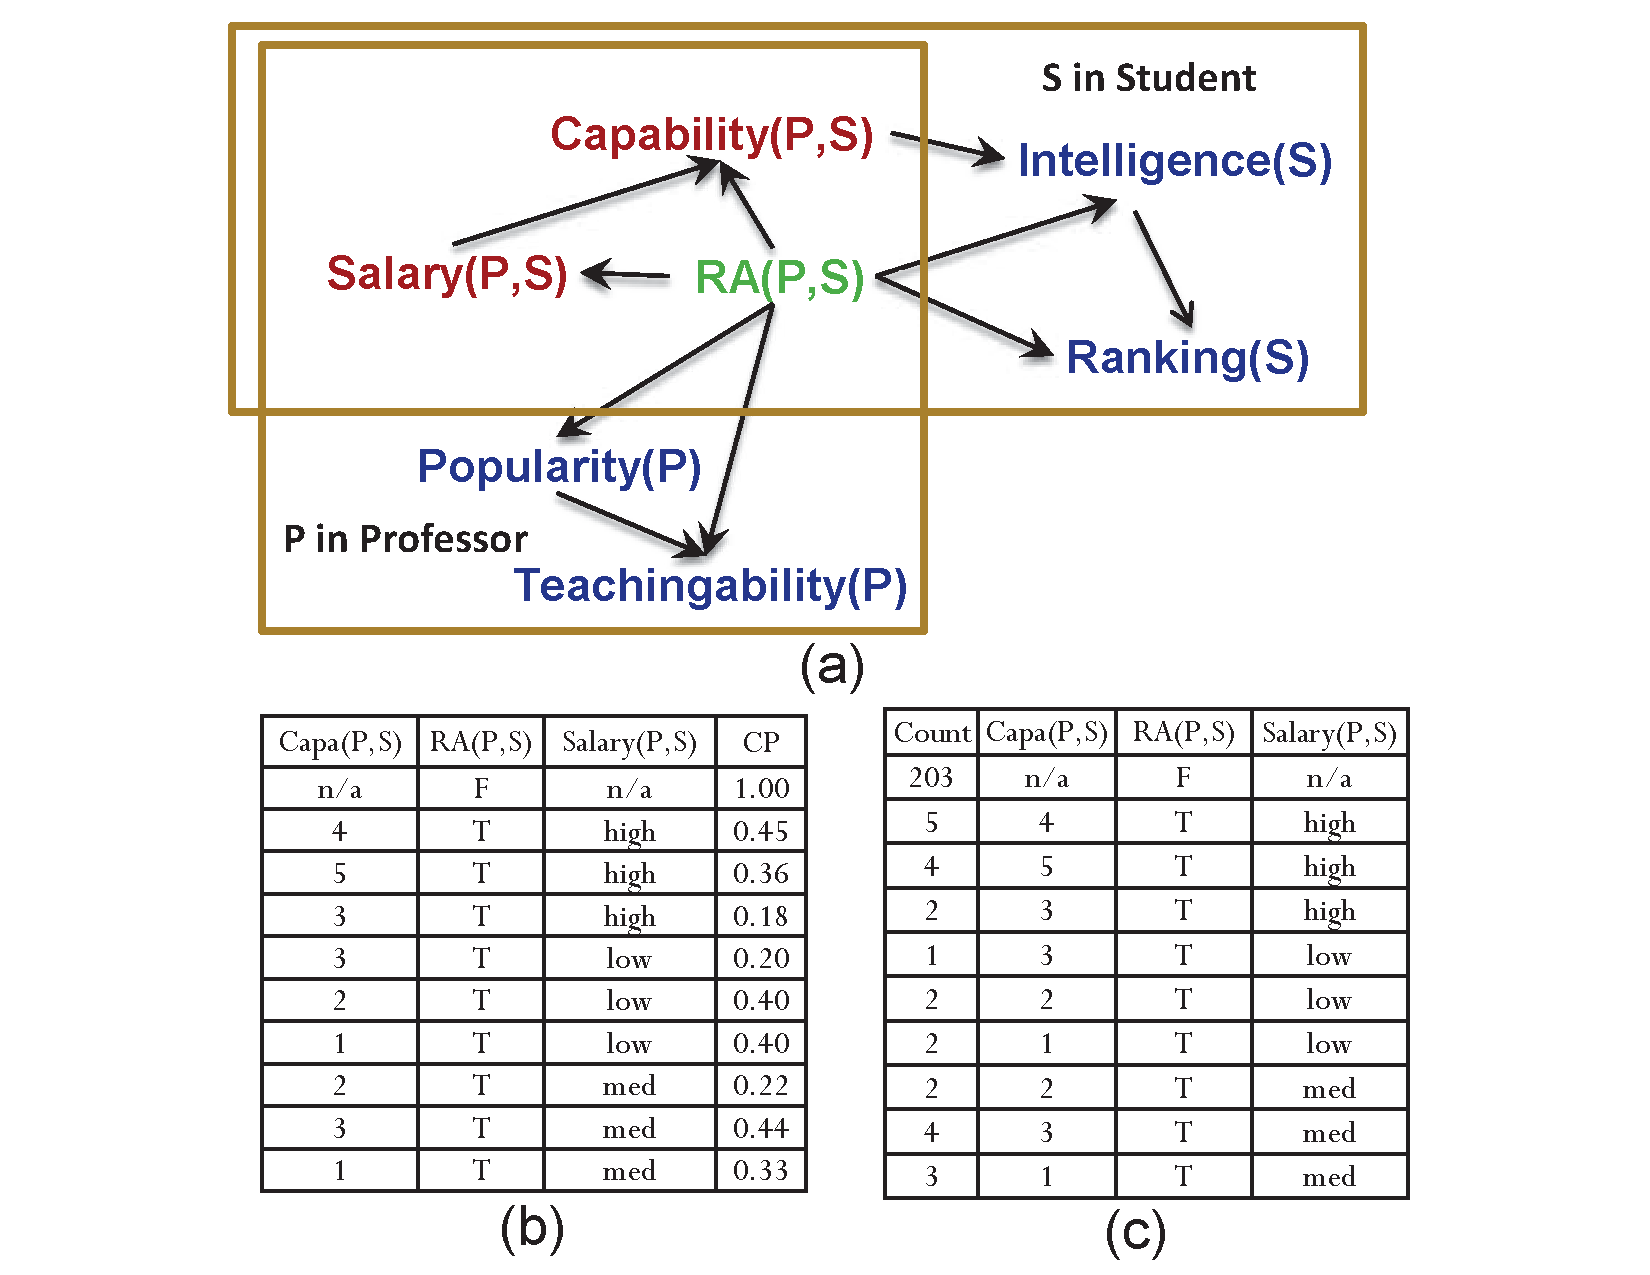
\includegraphics[width=0.5\textwidth]{pbn.pdf} 
%} 
%\caption{(a) Bayesian network for the University domain. (b) Conditional Probability table $Capability(\P,\S)\_\cptable$, for the node $Capability(\P,\S)$. Only value combinations that occur in the data are shown. (c) Contingency Table $Capability(\P,\S)\_\cttable$ for the node $Capability(\P,\S)$ and its parents. Both CP and CT tables are stored as database tables.
%}
% \label{fig:pbn}
%\label{fig:ct-cp-table}
%\end{figure}
%

%\begin{figure}[htbp] %  figure placement: here, top, bottom, or page
% \centering
%\resizebox{0.4\textwidth}{!}{
% \includegraphics[width=0.5\textwidth]{ct-cp-table.pdf} 
%} 
%\caption{ct-cp-table}
% \label{fig:ct-cp-table}
%\end{figure}

%\subsection{Model Representation} 




\subsection{Parameter Manager} \label{sec:parameters}

Deriving predictions from a model requires estimating values for its parameters.  Maximizing the data likelihood is the basic parameter estimation method for Bayesian networks. The maximum likelihood estimates equal the observed frequency of a child value given its parent values.
% \cite{Schulte2012}. 

%\paragraph{SQL Construction of Conditional Probability Tables} 
{\em SQL Implementation With Natural Join.} Given the sufficient statistics in a contingency table, a conditional probability table containing the maximum likelihood estimates can be computed by aggregation using SQL as in the example below. 

\begin{alltt}
SELECT count/temp.parent\_count as CP, 
capability(P,S), RA(P,S), salary(P,S) 
FROM capability(P,S)\_CT 
NATURAL JOIN  
(SELECT sum(Count) as parent\_count, 
RA(P,S), salary(P,S) 
FROM capability(P,S)\_CT  
GROUP BY  RA(P,S), salary(P,S) ) as temp
\end{alltt}


%\textbf{Zhensong: how about showing the SQL query that does this for the example in Figure~\ref{fig:pbn}? I think this clearer, shorter and easier to read.}
%
%More complex smoothing methods such as the Laplace correction can be easily computed from the maximum likelihood estimates. 
%[\textbf{Zhensong}: should this be an algorithm rather than a list? chaning to algorithm would take more space. I prefer to use list.]
%
%\begin{enumerate}
%\item For each node, construct a \textbf{local contingency table} whose par-RV set comprises the node and its parents. 
%This table can be computed by marginalization (Group By using the joint contingency table.
%%from scratch using the count manager, or may already be available as part of model structure learning (see below). 
%\item Construct a  parent contingency table whose par-RV set comprises the parents only. This table can be computed by marginalization using the local contingency table.
%%  On the local contingency table, apply a query with SUM(count) AS parent\_count in the Select clause and $\textless$parent-list$\textgreater$ in the GROUP BY clause. 
%\item Carry out a natural join of the local contingency table with the parent contingency table, dividing each local contingency count by the parent\_count. 
%%The natural join matches the values of parent variables. 
%\end{enumerate}


%%CREATE TABLE IF NOT EXISTS capability(p,s)\_CP
%\begin{alltt}
%SELECT 
%capability(p,s)\_CT.count/temp.count\_sum as CP, 
%capability(p,s)\_CT.capability(p,s), 
%capability(p,s)\_CT.RA(p,s), 
%capability(p,s)\_CT.salary(p,s) 
%FROM capability(p,s)\_CT 
%NATURAL JOIN  
%(SELECT sum(Count) as count\_sum, 
%RA(p,s), salary(p,s) 
%FROM capability(p,s)\_CT  
%GROUP BY  RA(p,s), salary(p,s) ) as temp
%\end{alltt}
%CREATE TABLE IF NOT EXISTS capability(p,s)\_CP
%\begin{alltt}
%SELECT count/temp.parent\_count as CP, 
%capability(P,S), capability(P,S)\_CT.RA(P,S), 
%capability(P,S)\_CT.salary(P,S) 
%FROM capability(P,S)\_CT 
%NATURAL JOIN  
%(SELECT sum(Count) as parent\_count, 
%RA(P,S), salary(P,S) 
%FROM capability(P,S)\_CT  
%GROUP BY  RA(P,S), salary(P,S) ) as temp
%\end{alltt}
%All of these tables can be stored as views. 
%This means that parameter values are updated automatically when contingency tables are updated, that is, when new data are obtained. 
%For statistical models without closed-form estimation formulas, such as Markov Logic Networks, parameter learning requires a local search. In this case a program would be needed to compute parameter estimates and store them in the factor tables. RDBMS support for parameter estimation procedures has been explored \cite{Feng_SIGMOD_2012,Niu2011,Niu2011a}.
%Figure~\ref{fig:ct-cp-table} shows a local contingency table and a conditional probability table for the node Capability(P, S). 








%As the top level of  Figure~\ref{fig:flow} illustrates, 
%The required counts involving only true relationships can be computed using the standard SQL constructs COUNT(*) and GROUP BY. 
%The general form of these operations is the same for every input database. 
%The varying part is the list of columns to be included, which depends on the input database. 
%For a fixed database, the column lists can be hard-coded. 
%To achieve a general solution when the column list is not known in advance, we introduce a new approach that we refer to as an SQL \textbf{metaquery}. 
%Thus an SQL metaquery maps schema information to the components of another SQL query. 
 
\subsection{Model Score Computation} \label{sec:model-score}
% oops, the model likelihood is undefined.
%Model structure learning uses a model selection score to find an optimum model for a given database (line xxx of Algorithm~\ref{alg:learning}). 
%Model selection scores can be computed and stored in an RDBMS as well. Caching model selection scores is important for scalable structure learning \cite{Russell2010}. 
A typical model selection approach is to maximize the likelihood of the data, balanced by a penalty term. For instance, the Akaike Information Criterion (AIC) is defined as follows %\cite{Domingos2009}
%check reference, was Witten before
\[
\mathit{AIC}(\G,\D) \equiv ln(P_{\widehat{G}}(\D)) - \parameters(\G) \]
where $\widehat{G}$ is the BN $\G$ with its parameters instantiated to be the maximum likelihood estimates given the database $\D$, and $\parameters(\G)$ is the number of free parameters in the structure $\G$. 
The number of free parameters for a node is the product of (the possible values for the parent nodes) $\times$ (the number of the possible values for the child node -1). Given the likelihood and the number of parameters, the AIC column is computed as $\aic = \loglikelihood - \parameters$. 
%These values can be inserted directly or the AIC column can be implemented as a derived column. 
 Model selection scores other than AIC can be computed in a similar way given the model likelihood and number of parameters.
%One complication is that if a relationship node has the value $\false$, then all associated 2Variables (relationship attributes) must have the value n/a. The computation of the number of parameters must be adjusted to account for this deterministic relationship; for the details see the script in the supplementary material. 
%We discuss how to use SQL for computing each.

\subsubsection{Parameter Number Computation} To determine the number of parameters of the child node @parVar-ID@, the number of possible child and parent values can be found from the $\it{\RVD.Domain}$ table in the Random Variable Database.  
%The $\parameters$ number for  is also inserted into the $\it{Scores}$ table. 

\subsubsection{Likelihood Computation} As explained in Section~\ref{sec:log-linear}, the log-likelihood can be computed by multiplying the instantiation counts of a factor by its value. Assuming that instantiation counts are represented in a contingency table and factor values in a factor table, this multiplication can be elegantly performed using the Natural Join operator. For instance, the log-likelihood score associated with the $Capability(\P,\S)$ family is given by the SQL query below. The aggregate computation in this short query illustrates how well SQL constructs support complex computations with structured objects. 

\begin{alltt}
SELECT Capability(P,S),  SUM
(MDB.Capability(P,S)\_CPT.cp * \\CDB.Capability(P,S)\_CT.count) 
AS loglikelihood
FROM MDB.Capability(P,S)\_CPT 
NATURAL JOIN CDB.Capability(P,S)\_CT
\end{alltt}


%
%Assume that the maximum likelihood estimates are represented in a conditional probability table (Section~\ref{sec:parameters}). For a BN $\G$, the log-likelihood function $ln(P_{\widehat{G}}(\D))$ can be computed node by node, as follows \cite{Schulte2011}. For each child node value, and for each combination of parent values: (1) find the instantiation count in the data for the conjunction of child node value and parent node values. (2) Find the conditional probability of the child node value given the parent node values. (3) Multiply the instantiation count by the logarithm of the conditional probability. Finally, sum these products to obtain a total likelihood score for the child node.
%
%{\em SQL Implementation.} The model manager supports this computation as follows. We assume that for each node with ID $@nodeID@$, a conditional probability database table $@nodeID@\_\cptable$ has been built in the Models database $\MDB$. Similarly, we assume that
%a local contingency database table $\CDB.@nodeID@\_\cttable$ has been built in the Count Database $\CDB$. The model likelihood for node $@nodeID@$ can be computed in SQL simply using the natural join of the two tables summing over a row-wise product, as follows. The $\loglikelihood$ value for $@nodeID@$ is inserted into the $\it{Scores}$ table. 
%\begin{alltt}
%SELECT @nodeID@,  SUM
%(MDB.@nodeID@\_CPT.cp * CDB@nodeID@\_CT.count) 
%AS loglikelihood
%FROM MDB.@nodeID@\_CPT 
%     NATURAL JOIN CDB.@nodeID@\_CT
%\end{alltt}
%our system creates a view $@nodeID@\_Likelihood$. This view has the same schema as the CP database table $@nodeID@\_\cptable$, except that instead of a conditional probability for a given child-parent configuration, we store a likelihood score. 
%We assume that a local contingency database table $\ct$ and a conditional probability database table $\cptable$ have been built for the child node as describe above (see Figure~\ref{fig:ct-cp-table}). The model likelihood can be computed in SQL simply as the natural join of the two tables, with a new column $\it{likelihood}$ defined by $$\it{likelihood} = \it{ct.count} * log(\cptable.\cp).$$ 

It is possible to extend the model manager to handle the multi-net structure learning method of the learn-and-join algorithm~\cite{Schulte2012}. The algorithm learns multiple Bayesian networks and propagates edges among them. The $\MDB$ schema is easily extended to store multiple Bayesian networks in a single table. The edge propagation can be executed by the RDBMS using the view mechanism. For more details, please see~\cite{bib:bbsite}. 

This completes our description of how the modules of \FB\ are implemented using SQL. We next show how these modules support a key learning task: computing the predictions of an SRL model on a test instance. 
%Computing the multi-relational likelihood in a general programming language (e.g., Java) would require significant development effort and result in a solution that is less concise, portable, and reliable.

%Given the table $\it{BayesNet}$ that specifies the Bayes net graph, we create a view $\it{NumParameters}$ whose columns are $\it{Node}$ and $\it{Parameters}$. An entry such as $(\it{Capability}(\P,\S),16)$ means that the number of parameters associated with the capability node in the BN model is 16. 
%
 %




\section{Test Set Predictions} Computing probabilities over the label of a test instance is important for several tasks. 1) Classifying the test instance, which is one of the main applications of a machine learning system for end users. 2) Comparing the class labels predicted against true class labels is a key step in several approaches to model scoring \cite{Kimmig2015}. 3) Evaluating the accuracy of a machine learning algorithm by the train-and-test paradigm, where the system is provided a training set for learning and then we test its predictions on unseen test cases. %
%
We first discuss how to compute a prediction for a single test case, then how to compute an overall prediction score for a set of test cases. Class probabilities can be derived from Equation~\ref{eq:parfactor} as follows \cite[Sec.2.2.2]{Kimmig2015}. Let $\Y$ denote a ground par-RV to be classified, which we refer to as the \textbf{target variable}. For example, a ground atom may be $\it{Intelligence}(jack)$. In this example, we refer to jack as the \textbf{target entity}. Write $\set{X}_{-\Y}$ for a database instance that specifies the values of all ground par-RVs, except for the target, which are used to predict the target node. Let $[\set{X}_{-\Y},\y]$ denote the completed database instance where the target node is assigned value $\y$. The log-linear model uses the likelihood $P([\set{X}_{-\Y},\y])$ as the joint score of the label and the predictive features. The conditional probability is proportional to this score:
\begin{equation} \label{eq:classify}
P(\y|\set{X_{-\Y}}) \propto P([\set{X}_{-\Y},\y])
\end{equation}
where the joint distribution on the right-hand side is defined by Equation~\ref{eq:parfactor}, and the scores of the possible class labels need to be normalized to define  conditional probabilities. 


%\subsection{SQL Computation of the Log-Linear Classification Score}
{\em SQL Implementation.} 
The obvious approach to computing the log-linear score would be to use the likelihood computation of Section~\ref{sec:model-score} for the entire database.
%to find the score $P_{G}(\set{X}_{-\Y,\y})$, then normalize. 
This is inefficient because only instance counts that involve the target entity change the classification probability. 
%For example, if jack is the target entity, then the grades of jill do not matter. 
This means that we need only consider query instantiations that match the appropriate logical variable with the target entity (e.g., $\S = jack$). 
%We show how the log-likelihood computation of Section~\ref{sec:model-score} can be adapted to compute a log-linear classification score for a set of target entities. 
%This illustrates how the modularity of \FB\ supports reusing its components for different tasks. 

For a given set of random variables, target entity instantiation counts can be represented in a contingency table that we call the \textbf{target contingency table}. Figure~\ref{fig:targetct} shows the format of a contingency table for target entities jack resp. jill.

\begin{table*}[t]
\caption{SQL queries for computing target contingency tables supporting test set prediction.  $\textless$Attribute-List$\textgreater$ and  $\textless$Key-Equality-List$\textgreater$ are as in Figure~\ref{fig:meta-query}.}
\begin{center}
\begin{tabular}{|c|p{6cm}|p{5cm}|p{4cm}}
Access &SELECT&WHERE&GROUP BY\\\hline
Single &COUNT(*) AS count, $\textless$Attribute-List$\textgreater$, S.sid& $\textless$Key-Equality-List$\textgreater$ AND S.s\_id = jack&  $\textless$Attribute-List$\textgreater$\\
\hline
Block & COUNT(*) AS count,  $\textless$Attribute-List$\textgreater$, S.sid& $\textless$Key-Equality-List$\textgreater$ &  $\textless$Attribute-List$\textgreater$, S.sid\\
\end{tabular}
\end{center}
\label{table:target-query}
\end{table*}%

\begin{figure}[htbp] %  figure placement: here, top, bottom, or page
 \centering
\resizebox{0.35\textwidth}{!}{
 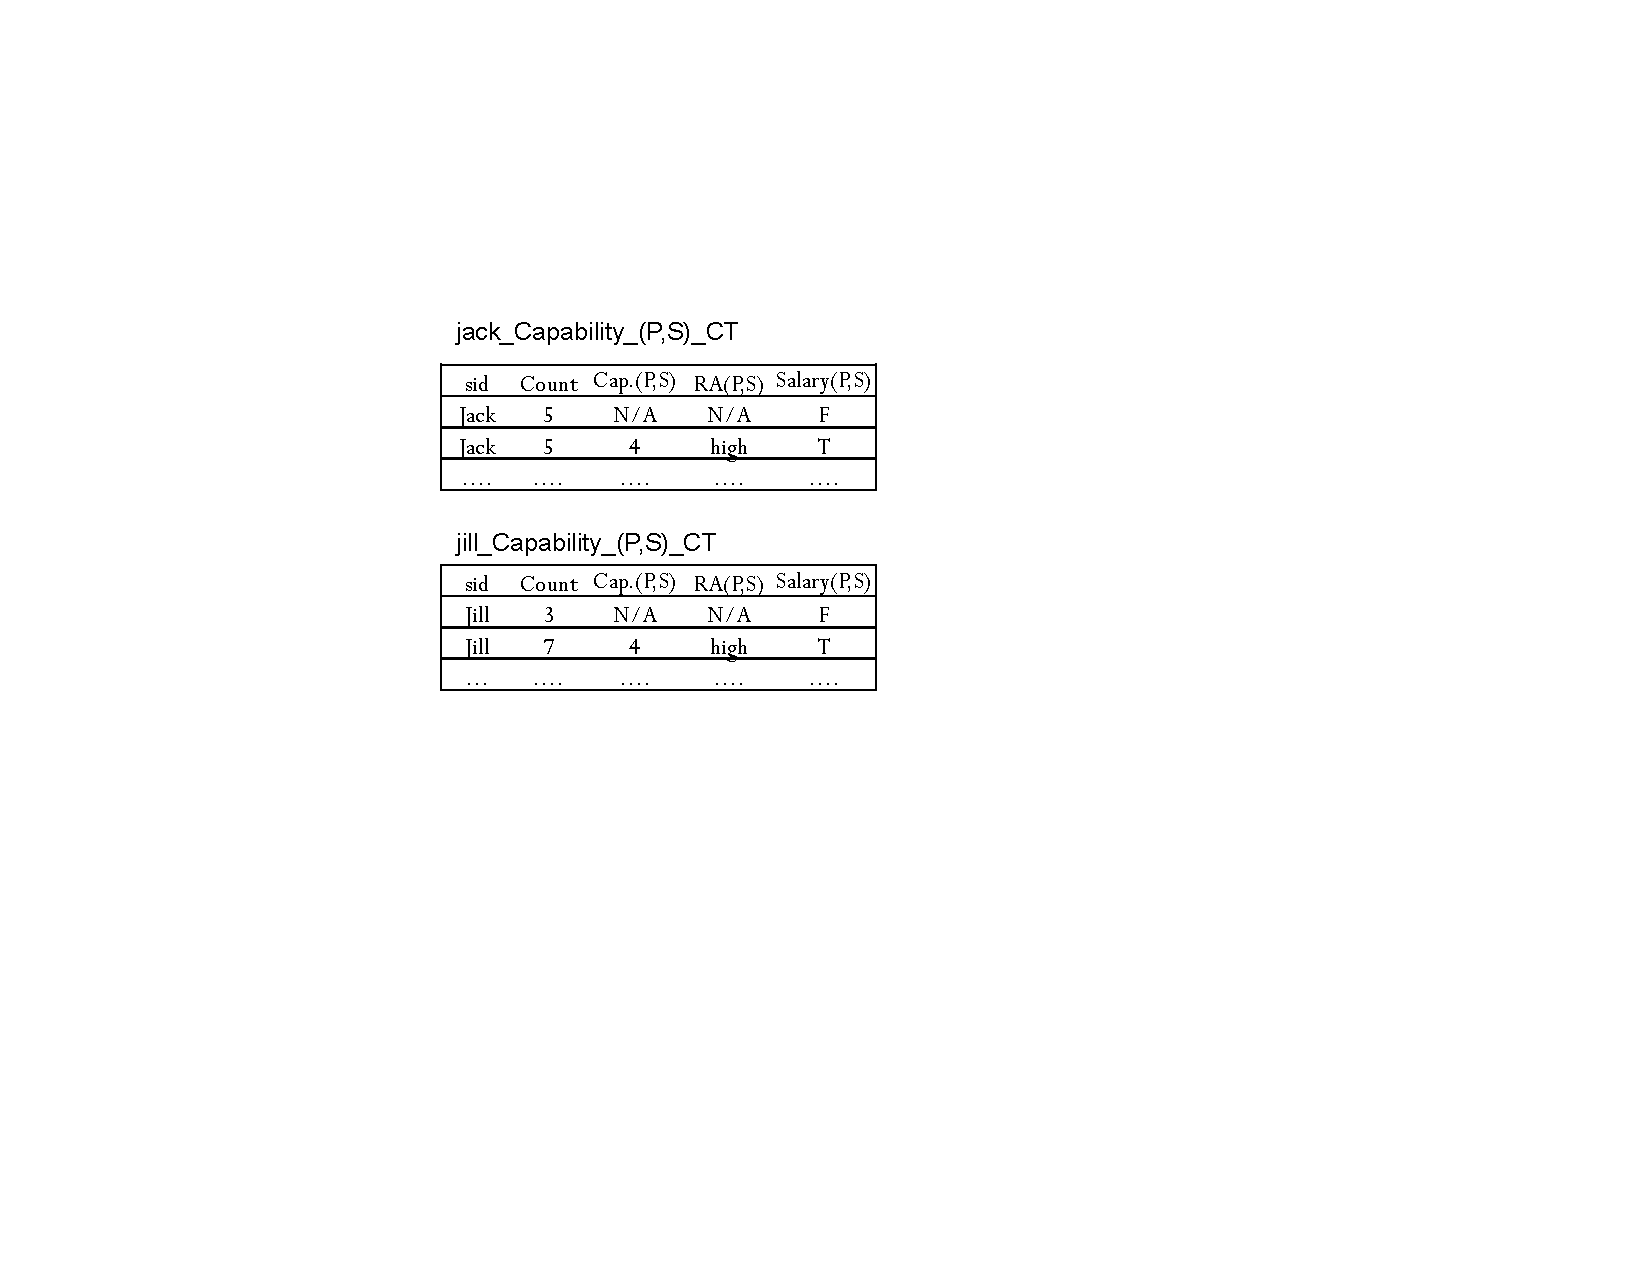
\includegraphics{targetct} 
} 
\caption{Target contingency tables for target = jack and for target = jill.}
 \label{fig:targetct}
\end{figure}

{\em Assuming} that for each node with ID @parRVID@, a target contingency table named $\CDB.target\_@\it{parRVID}@\_\cttable$ has been built in the Count Database $\CDB$, the log-likelihood SQL is as in Section~\ref{sec:model-score}. For instance, the contribution of the $Capability(\P,\S)$ family is computed by the SQL query shown,  but with the contingency table jack\_Capability(P,S)\_CT in place of Capability(P,S)\_CT.
%\begin{alltt}
%SELECT @par-RVID@,  SUM (MDB.@par-RVID@\_CPT.CP 
%	* CDB.@par-RVID,	target@\_CT.count) 
%AS loglikelihood
%FROM MDB.@par-RVID@\_CPT 
%	NATURAL JOIN CDB.@par-RVID,target@\_CT
%\end{alltt}
%The conditional probability database table $@par-RVID,target@\_\cptable$ can be found in the Models database $\MDB$. (Notice that the conditional probabilities do not depend on the target entity, only on the model.)  
%This query computes the classification score for a BN node, the total score is the sum over BN nodes. 
%As is well-known in Bayes net theory, we need only sum scores for the target node and its children \cite{Neapolitan2004}. 
%
The new problem is finding the target contingency table. SQL allows us to solve this easily by restricting counts to the target entity in the WHERE clause. To illustrate, suppose we want to modify the contingency table query of Figure~\ref{fig:meta-query} to compute the contingency table for $\S = jack$. We add the student id to the SELECT clause, and the join condition $S.s\_id = jack$ to the WHERE clause; see Table~\ref{table:target-query}.%\footnote{Omit apostrophes for readability.} 
The FROM clause is the same as in Figure~\ref{fig:meta-query}. The metaquery of Figure~\ref{fig:meta-query} is easily changed to produce these SELECT and WHERE clauses.
%CLAUSES. 


%First we add the student id to the SELECT clause, so the new SELECT clause becomes
%
%\begin{alltt}
%COUNT(*) AS count, popularity(P), teachingability(P),
%intelligence(S), ranking(S), \em{S.sid}
%\end{alltt}
%
%and the new WHERE list becomes
%
%\begin{alltt}
%RA.p\_id = P.p\_id AND RA.s\_id = S.s\_id AND \em{S.s\_id = jack}.
%\end{alltt}

%We emphasize the new parts of the queries and omit apostrophes for readability. 
%
Next consider a setting where a model is to be scored against an entire test set. 
%This occurs for instance in the standard cross-validation computation for model scoring. 
For concreteness, suppose the problem is to predict the intelligence of a set of students
 $\it{Intelligence}(jack)$, $\it{Intelligence}(jill)$,
 $\it{Intelligence}(student_{3}),\ldots, \it{Intelligence}(student_{m})$.
% An obvious approach is to loop through the set of test instances, repeating the likelihood query above for each single instance. Instead, 
 SQL supports {\em block access} where we process the test instances as a block. Intuitively, instead of building a contingency table for each test instance, we build a single contingency table that stacks together the individual contingency tables (Figure~\ref{fig:targetct}). Blocked access can be implemented in a beautifully simple manner in SQL: we simply add the primary key id field for the target entity to the GROUP BY list; see Table~\ref{table:target-query}. 
%To illustrate,  suppose for simplicity that the $\it{Student}$ table contains all test target entities. The query for the stacked contingency table is constructed as in Figure~\ref{fig:meta-query}, with the change that: We add the $\it{S.sid}$ field to the SELECT and to the GROUP BY lists. The FROM and WHERE clauses are as in Figure~\ref{fig:meta-query}. 
 %
%In contrast, programming blocked access in a general purpose programming language would require significant development effort and probably new file or data structures. If the set of test instances is large, a stacked contingency table is also unlikely to fit into main memory.
  %

\section{Evaluation} 

Our experimental study describes how \FB\ can be used to implement a challenging machine learning application: Constructing a Bayesian network model for a relational database. Bayesian networks are a good illustration of typical challenges and how RDBMS capabilities can address them because: (1) Bayesian networks are widely regarded as a very useful model class in machine learning and AI, that supports decision making and reasoning under uncertainty. At the same time, they are considered challenging to learn from data. (2) Database researchers have proposed Bayesian networks for combining databases with uncertainty %\cite{Wang2008,Deshpande_VLDB2007}
\cite{Wang2008}. (3) A Bayesian network with par-RVs can be easily converted to other first-order representations, such as a Markov Logic Network; see \cite{Domingos2009}.

We describe the system and the datasets we used.
Code was written in MySQL Script and Java, JRE 1.7.0.  and executed with 8GB of RAM and a single Intel Core 2 QUAD Processor Q6700 with a clock speed of 2.66GHz (no hyper-threading). The operating system was Linux Centos 2.6.32. 
The MySQL Server version 5.5.34 was run with 8GB of RAM and a single core processor of 2.2GHz. 
All code and datasets are available on-line \cite{bib:bbsite}. 


\subsection{Datasets} \label{sec:datasets}
We used six benchmark real-world databases. For detailed descriptions and  the sources of the databases, please see ~\cite{bib:bbsite} and the references therein. Table~\ref{table:datasetsize} summarizes basic information about the benchmark datasets.  
IMDb is the largest dataset in terms of number of total tuples (more than 1.3M tuples) and schema complexity. %attributes.
It combines the MovieLens database\footnote{www.grouplens.org, 1M version} with data from the Internet Movie Database (IMDb)\footnote{www.imdb.com, July 2013} following \cite{Peralta2007}. 


\begin{table}[hbtp]
\caption{Datasets characteristics. \#Tuples = total number of tuples over all tables in the dataset. }
 \centering
%\scalebox{0.7in}{
\resizebox{0.5\textwidth}{!}{
\begin{tabular}[c]
{|l|c|c|r|c|}\hline
 \textbf{Dataset} & \textbf{\begin{tabular}[l] {ll} \#Relationship \\Tables/ Total \end {tabular}} & \textbf{\begin{tabular}[l] {ll} \# par-RV \end {tabular}}  & \textbf{\#Tuples} 
%& \textbf{\#Attributes}  
\\\hline
% \textbf{Dataset} & \textbf{Relationships} & \textbf{\begin{tabular}[l] {ll} Self \\Relationships \end {tabular}} &
% \textbf{\begin{tabular}[l] {ll} Same Type\\ Relationships \end {tabular}}& \textbf{\#Tuples} & \textbf{\begin{tabular}[l] {ll} \#Attribute  \\Columns \end{tabular}}  \\\hline
 %   University&2 & 0 & N & 171 & 12\\\hline
    Movielens &1 / 3 & 7  & 1,010,051 
%& 7
\\\hline
%    Movielens(0.1M) &1 & N & N &  83,402 & 7\\\hline
    Mutagenesis & 2 / 4 & 11 & 14,540 
%& 11
\\\hline
 UW-CSE &2 / 4 & 14  & 712 %& 14
\\\hline   
  Mondial &2 / 4 & 18 &  870
%& 18
\\\hline
    %Financial &3 / 7 & 0  &  225,932& 15\\\hline
   Hepatitis &3 / 7 & 19 &12,927  
%& 19
\\\hline
   IMDb &3 / 7 & 17 &1,354,134  %& 17
\\\hline   
\end{tabular}
}
 % end scalebox

  \label{table:datasetsize}
\end{table}

Table~\ref{table:datasetsize} provides information about the number of par-RVs generated for each database. More complex schemas 
%and self-relationships 
generate more random variables. 
%
%The metadata requires little storage. The reason for using an RDBMS to store it is not because it requires large memory, but because relational algebra is an excellent language for manipulating structured objects.

%% Table generated by Excel2LaTeX from sheet 'model-manager'
%\begin{table}[htbp] \caption{Random variable database statistics. \textbf{Zhensong: please merge with table above.}}
%  \centering
%    \begin{tabular}{|l|c|}
%    \hline
%    	extbf{Dataset} &	extbf{\# par-RV}\\
%    \hline
%    Movielens & 7     \\
%    \hline
%    Mutagenesis & 11    \\
%    \hline
%    UW-CSE & 14    \\
%    \hline
%    Mondial & 18    \\
%    \hline
%    Hepatitis & 19    \\
%    \hline
%    IMDb  & 17    \\
%    \hline
%    \end{tabular}%
%  %
%  \label{tab:rvd}
%\end{table}%
%



%% Table generated by Excel2LaTeX from sheet 'Sheet1'
%\begin{table}[htbp]
%  \centering
%   \resizebox{0.5\textwidth}{!}{ \begin{tabular}{|l|r|r|r|r|r|}
%    \hline
% \textbf{  Dataset  }&  \textbf{ \begin{tabular}[l] {ll} \# Database\\Tuples  \end{tabular} }&\textbf{ \begin{tabular}[l] {ll}\# Sufficient \\ Statistics \end{tabular}}& \textbf{\begin{tabular}[l] {ll} SS \\Computing\\ Time (s) \end{tabular}} &\textbf{\begin{tabular}[l] {ll}  \#BN \\ Parameters  \end{tabular}} & \textbf{\begin{tabular}[l] {ll}Para. \\Learning\\ Time (s) \end{tabular} }\\
%    \hline
%    Movielens & 1,010,051 & 252   & 2.7   & 292   & 0.57  \\
%    \hline
%    Mutagenesis & 14,540 & 1,631 & 1.67  & 721   & 0.98  \\
%    \hline
%    UW-CSE & 712   & 2,828 & 3.84  & 241   & 1.14  \\
%    \hline
%    Mondial & 870   & 1,746,870 & 1,112.84 & 339   & 60.55  \\
%    \hline
%%    Financial & 225,932 & 3,013,011 & 1,421.87 & 2,433  & 88.974  \\
%%    \hline
%    Hepatitis & 12,927 & 12,374,892 & 3,536.76 & 569   & 429.15  \\
%    \hline
%    IMDb  & 1,354,134 & 15,538,430 & 7,467.85 & 60,059 & 505.61  \\
%    \hline
%    \end{tabular}%
%}
%  \label{tab:addlabel}%
%  \caption{Count Manager}
%\end{table}%

% Table generated by Excel2LaTeX from sheet 'Sheet1'

\subsection{Bayesian Network Learning} 
For learning the structure of a first-order Bayesian network, we used \FB\ to implement the previously existing learn-and-join algorithm (LAJ). 
%The LAJ method takes as input a joint contingency table for all relational random variables in the  database, which we computed using the Count Manager. 
The model search strategy of the LAJ algorithm is an iterative deepening search for correlations among attributes along longer and longer chains of relationships. For more details please see \cite{Schulte2012}. 
The previous implementation of the LAJ algorithm posted at~\cite{bib:bbsite}, limits the par-factors so they contain at most {\em two} relationship par-RVs; \FB\ overcomes this limitation.

A major design decision is how to make sufficient statistics available to the LAJ algorithm. In our experiments we followed a {\em pre-counting} approach where the count manager constructs a \textbf{joint contingency table} for {\em all} par-RVs in the random variable database. An alternative would be {\em on-demand} counting, which computes many contingency tables, but only for factors that are constructed during the model search \cite{Lv2012}.
% \textbf{Zhensong: reference}. 
%For example, if there is a total of $n$ par-RVs, the number of columns in the joint contingency table is $n$. But if model search never considers factors that involve all $n$ par-RVs, then on-demand counting never constructs a contingency table of size $n$. 
%On-demand counting trades off the upfront cost of constructing a large contingency table against the cost of computing many %different 
%small contingency tables. 
Pre-counting is a form of data preprocessing: Once the joint contingency table is constructed, local contingency tables can be built quickly by summing (Group By). Different structure learning algorithms can therefore be run quickly on the same joint contingency table. 
%If the number of par-RVs is very large, on-demand counting is necessary. (reference et al.) examine the trade-offs between pre-counting and on-demand counting for single-table learning. We leave an investigation of the trade-offs for SRL for future work. \FB\ supports both approaches. 
%
For our evaluation, pre-counting has several advantages. (1) Constructing the joint contingency table presents a maximally challenging task for the count manager. (2) Separating counting/data access from model search allows us to assess separately the resources required for each task.

\subsection{Results}
Table~\ref{tab:counts} reports the number of sufficient statistics for constructing the joint contingency table. This number depends mainly on the number of par-RVs. The number of sufficient statistics can be quite large, over 15M for the largest dataset IMDb. 
%RDBMS support is key for managing counts in such cases. 
Even with such large numbers, constructing contingency tables using the SQL metaqueries is feasible, taking just over 2 hours for the very large IMDb set. 
The number of Bayesian network parameters is much smaller than the number of sufficient statistics.
%because it depends mainly on the indegree in the model graph. 
%The Bayesian network therefore provides a compact representation of the statistical information in the joint contingency table \cite{Schulte2014}. %Schulte2014
The difference between the number of parameters and the number of sufficient statistics measures how compactly the BN summarizes the statistical information in the data. %\cite{Schulte2012}.  
Table~\ref{tab:counts} shows that Bayesian networks provide very compact summaries of the data statistics. For instance for the Hepatitis dataset, the ratio is  $12,374,892/569 > 20,000$. The IMDb database is an outlier, with a complex correlation pattern that leads to a dense Bayesian network structure.

\begin{table}[htbp]
  \caption{Count Manager: Sufficient Statistics and Parameters}
  \centering
   \resizebox{0.5\textwidth}{!}{ \begin{tabular}{|l|r|r|r|r|r|}
    \hline
 \textbf{  Dataset  }&  \textbf{ \begin{tabular}[l] {ll} \# Database\\Tuples  \end{tabular} }&\textbf{ \begin{tabular}[l] {ll}\# Sufficient \\ Statistics (SS) \end{tabular}}& \textbf{\begin{tabular}[l] {ll} SS \\Computing\\ Time (s) \end{tabular}} &\textbf{\begin{tabular}[l] {ll}  \#BN \\ Parameters  \end{tabular}}%& \textbf{\begin{tabular}[l] {ll}Para. \\Learning\\ Time (s) \end{tabular} }
\\
    \hline
    Movielens & 1,010,051 & 252   & 2.7   & 292   \\%& 0.57  \\
    \hline
    Mutagenesis & 14,540 & 1,631 & 1.67  & 721   \\%& 0.98  \\
    \hline
    UW-CSE & 712   & 2,828 & 3.84  & 241   \\%& 1.14  \\
    \hline
    Mondial & 870   & 1,746,870 & 1,112.84 & 339  \\% & 60.55  \\
    \hline
%    Financial & 225,932 & 3,013,011 & 1,421.87 & 2,433  & 88.974  \\
%    \hline
    Hepatitis & 12,927 & 12,374,892 & 3,536.76 & 569   \\%& 429.15  \\
    \hline
    IMDb  & 1,354,134 & 15,538,430 & 7,467.85 & 60,059 \\%& 505.61  \\
    \hline
    \end{tabular}%
}
 \label{tab:counts}
\end{table}%

Table~\ref{tab:model} shows that the graph structure of a Bayesian network contains a small number of edges relative to the number of parameters. 
%The reason for using an RDBMS to store the graph is again because relational algebra allows us to easily combine it with other statistical objects. 
The parameter manager provides fast maximum likelihood estimates for a given structure. 
This is because computing a local contingency table for a BN family is fast given the joint contingency table.
%the variable set for a local contingency tables for BN parameter estimation comprises only a child node and its parents, so it is much smaller than the variable set in the joint contingency table.
%

% Table generated by Excel2LaTeX from sheet 'model-manager'
\begin{table}[htbp]
\caption{Model Manager Evaluation.}
  \centering
      \resizebox{0.5\textwidth}{!}{ \begin{tabular}{|l|r|r|r|r|}
    \hline
     \textbf{ Dataset} %&  \textbf{ \begin{tabular}[l] {ll}\# Tuples In \\  RRVD \end{tabular} } 
&  \textbf{ \begin{tabular}[l] {ll} \# Edges in \\Bayes Net  \end{tabular} }& \textbf{ \begin{tabular}[l] {ll} \# Bayes Net \\ Parameters   \end{tabular} } & \textbf{\begin{tabular}[l] {ll}Parameter \\Learning\\ Time (s) \end{tabular} }\\
    \hline
    Movielens &   72    %& 12
    & 292 & 0.57  \\
    \hline
    Mutagenesis &   124   % & 57
    & 721 & 0.98  \\
    \hline
    UW-CSE &       112 %& 118
   & 241  & 1.14 \\
    \hline
    Mondial &       141 %& 126 
  & 339 & 60.55    \\
    \hline
    Hepatitis &       207%& 142 
  & 569  & 429.15   \\
    \hline
    IMDb  &      195 %& 217  
 & 60,059   & 505.61\\
    \hline
    \end{tabular}%
}  
  \label{tab:model}%
\end{table}%


Figure~\ref{fig:test-timing} compares computing predictions on a test set using an instance-by-instance loop, with a separate SQL query for each instance, vs. a single SQL query for all test instances as a block (Table~\ref{table:target-query}). Table \ref{tab:test-instance} specifies the number of  test instances for each dataset. We split each benchmark database into  80\% training data, 20\% test data. The test instances are the ground atoms of all descriptive attributes of entities.  The blocked access method is 10-100 faster depending on the dataset. The single access method did not scale to the large IMDb dataset (timeout after 12 hours).

\begin{table}[htbp]
\caption{\# of Test Instances }
  \centering
  \begin{tabular}{|r|r|r|r|r|r|r|} \hline
\textbf{Dataset}&Movielens&	Mutagenesis	& 	UW-CSE	&	Mondial&	Hepatitis&	 	IMDb \\ \hline
{\#instance}	&4,742	 	&	3,119		&576	&		505&2,376	 	&46,275 \\ \hline
    
\end{tabular}%  
  \label{tab:test-instance}%
\end{table}%

\begin{figure}[htbp] %  figure placement: here, top, bottom, or page
 \centering
\resizebox{0.4\textwidth}{!}{
 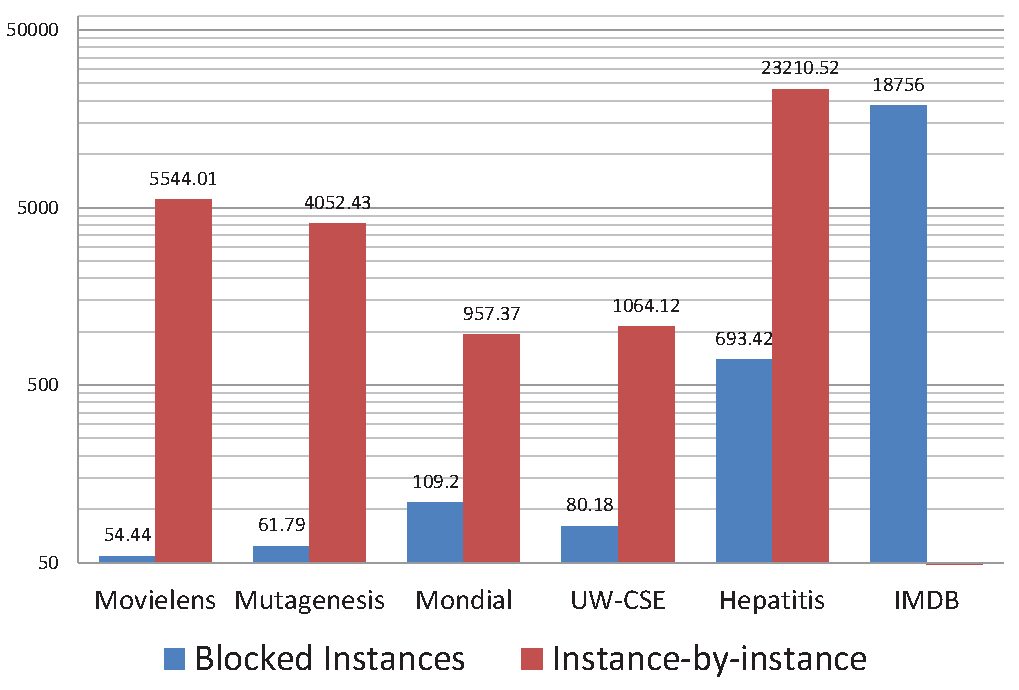
\includegraphics[width=0.5\textwidth]{test-timing.pdf} 
} 
\caption{Times (s) for Computing Predictions on Test Instances. The right red column shows the time for looping over single instances using the Single Access Query of Table~\ref{table:target-query}. The left blue column shows the time for the Blocked Access Query of Table~\ref{table:target-query}.
}
 \label{fig:test-timing}
\end{figure}

%\begin{table}[htbp]\caption{Model Manager Evaluation.}
%  \centering
%      \resizebox{0.5\textwidth}{!}{ \begin{tabular}{|l|r|r|r|r|}
%    \hline
%     \textbf{ Dataset} %&  \textbf{ \begin{tabular}[l] {ll}\# Tuples In \\  RRVD \end{tabular} } 
%&  \textbf{ \begin{tabular}[l] {ll} \# Tuples in \\Bayes Net  \end{tabular} }& \textbf{ \begin{tabular}[l] {ll} \# Bayes Net \\ Parameters   \end{tabular} } & \textbf{\begin{tabular}[l] {ll}Para. \\Learning\\ Time (s) \end{tabular} }\\
%    \hline
%    Movielens &   72    %& 12
%    & 292 & 0.57  \\
%    \hline
%    Mutagenesis &   124   % & 57
%    & 721 & 0.98  \\
%    \hline
%    UW-CSE &       112 %& 118
%   & 241  & 1.14 \\
%    \hline
%    Mondial &       141 %& 126 
%  & 339 & 60.55    \\
%    \hline
%    Hepatitis &       207%& 142 
%  & 569  & 429.15   \\
%    \hline
%    IMDb  &      195 %& 217  
% & 60,059   & 505.61\\
%    \hline
%    \end{tabular}%
%}  
%  \label{tab:model}%
%\end{table}%


Table~\ref{tab:othersrl} reports result for the complete learning of a Bayesian network, structure and parameters. It benchmarks \FB\ against functional gradient boosting, a state-of-the-art  multi-relational learning approach.
%~\cite{Natarajan2012}. 
MLN\_Boost learns a Markov Logic Network, and RDN\_Boost a Relational Dependency Network. 
We used the Boostr implementation \cite{Khot2013}. 
To make the results easier to compare across databases and systems, we divide the total running time by the number of par-RVs for the database (Table~\ref{table:datasetsize}). 
Table~\ref{tab:othersrl} shows that structure learning with \FB\ is fast: even the large complex database IMDb requires only around 8 minutes/par-RV. Compared to the boosting methods, \FB\ shows excellent scalability: neither boosting method terminates on the IMDb database, and while RDN\_Boost terminates on the MovieLens database, it is almost 5,000 times slower than {\sc FactorBase}. 
%While the Learn-and-Join model search  is more efficient than the boosting ensemble search, m
Much of the speed of our implementation is due to quick access to sufficient statistics. As the last column of Table~\ref{tab:othersrl} shows, on the larger datasets \FB\ spends about 80\% of computation time on gathering sufficient statistics via the count manager. This suggests that a large  speedup for the boosting algorithms could be achieved if they used the \FB\ in-database design. 

We do not report accuracy results due to space constraints and because predictive accuracy is not the focus of this paper. On the standard conditional log-likelihood metric, as defined by Equation~\ref{eq:classify}, the model learned by \FB\ performs better than the boosting methods on all databases. This is consistent with the results of previous studies \cite{Schulte2012}.

\begin{table}[htbp] \caption{Learning Time Comparison (sec) with other statistical-relational learning systems. NT = non-termination}
  \centering
      \resizebox{0.45\textwidth}{!}{
\begin{tabular}{|l|r|r|r|r|}\hline
Dataset  & RDN\_Boost  & MLN\_Boost  & FB-Total & FB-Count \\\hline
MovieLens & 5,562  & N/T & 1.12 & 0.39 \\\hline
Mutagenesis  & 118 & 49 & 1 & 0.15 \\\hline
UW-CSE & 15 & 19 & 1 & 0.27 \\\hline
Mondial  & 27 & 42 & 102 & 61.82 \\\hline
Hepatitis  & 251 & 230 & 286 & 186.15 \\\hline
IMDb & N/T & N/T & 524.25 & 439.29 \\\hline
\end{tabular}
} 
  \label{tab:othersrl}%
\end{table}%

{\em Conclusion.} \FB\ leverages RDBMS capabilities for scalable management of statistical analysis objects. It efficiently constructs and stores large numbers of sufficient statistics and parameter estimates. 
%MRLBase can integrate information from different statistical objects when they are maintained as first-class citizens in the RDBMS. 
The RDBMS support for statistical-relational learning translates into orders of magnitude improvements in speed and scalability.
% compared to other state-of-the-art methods.


\section{Related Work} \label{sec:related}

The design space for combining machine learning with data management systems offers a number of possibilities, several of which have been explored in previous and ongoing research. 
We selectively review the work most relevant to our research. Figure~\ref{fig:related} provides a tree structure for the research landscape. 

\begin{figure}[htbp] %  figure placement: here, top, bottom, or page
 \centering
\resizebox{0.4\textwidth}{!}{
 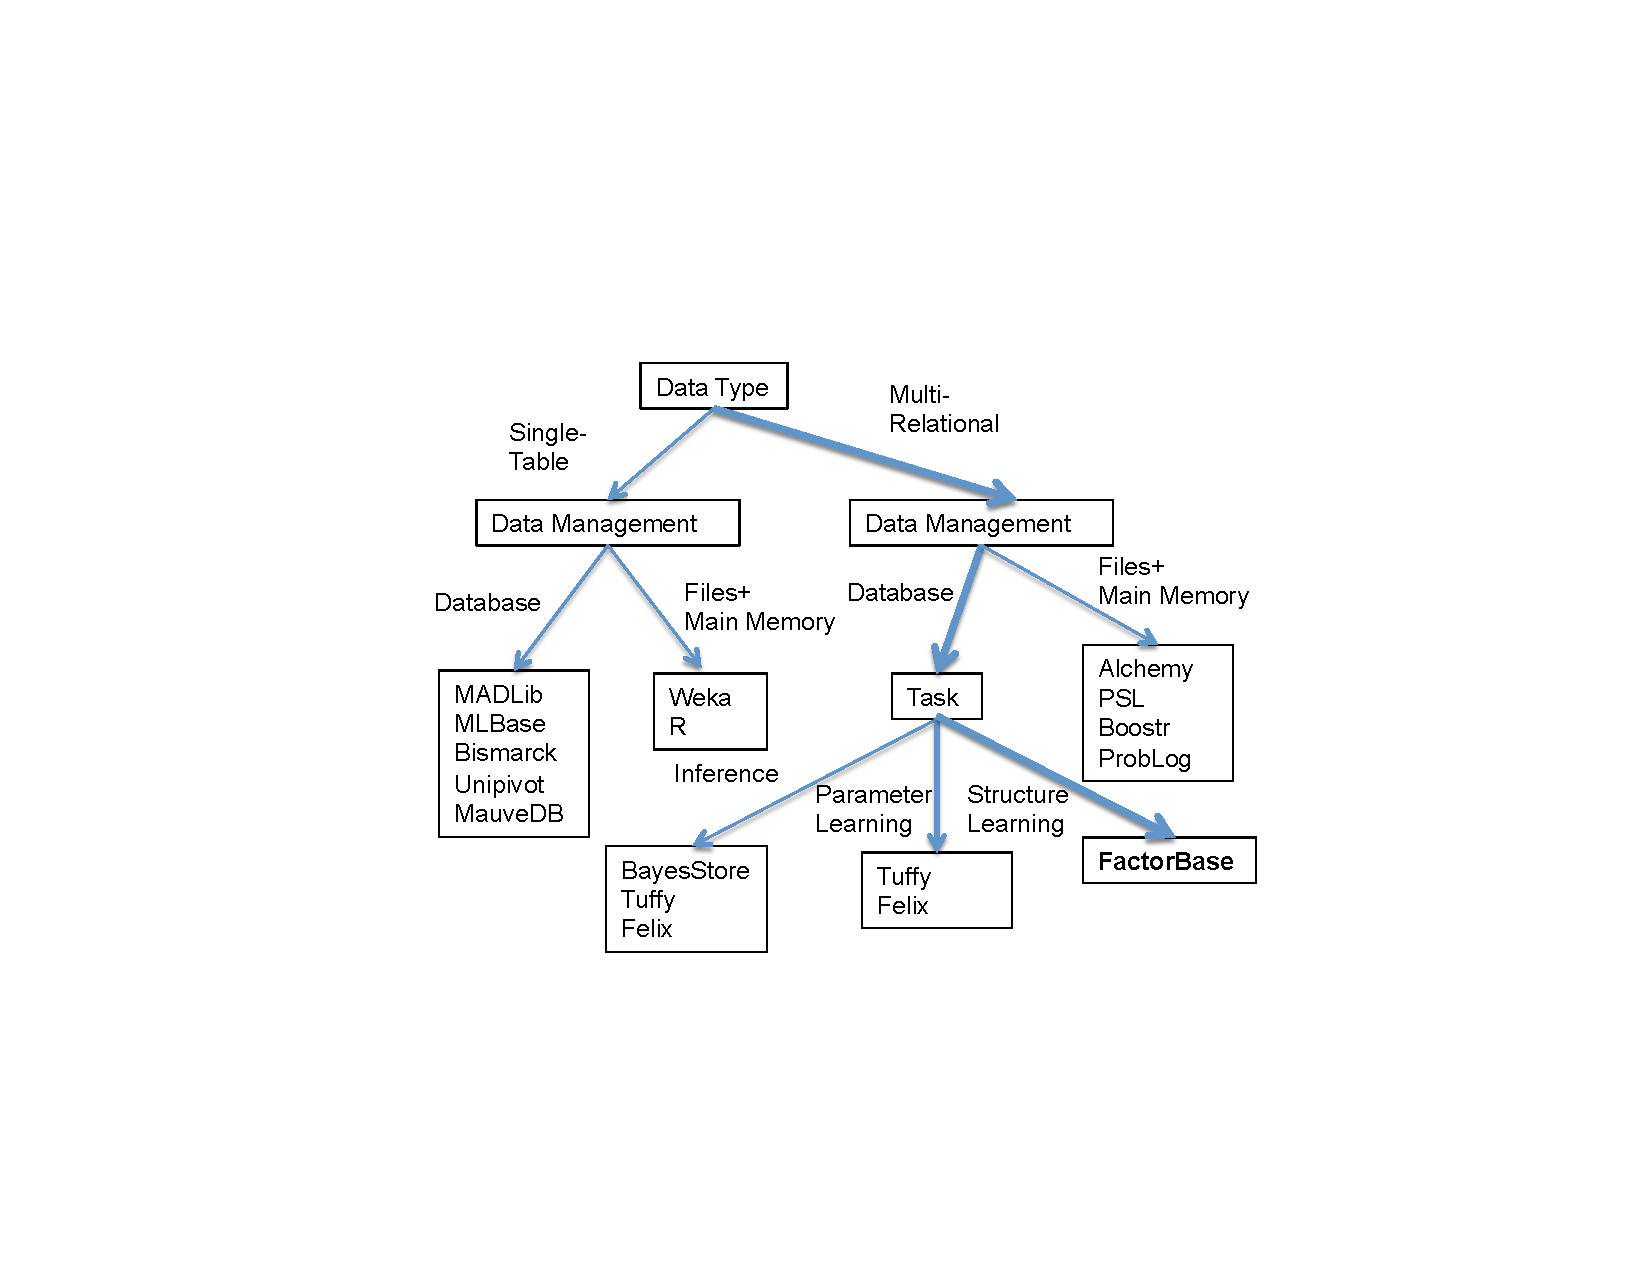
\includegraphics[width=0.5\textwidth]{related-dt.pdf} 
 }
\caption{A tree structure for related work in the design space of machine learning $\times$ data management}
\label{fig:related}
\end{figure}

%Given the density of the research landscape around the topics of machine learning and data management, Figure~\ref{fig:novelty} provides a graphical illustration of where MRLBase is located with respect to other work.
\subsection{Single-Table Machine Learning} Most machine learning systems, such as Weka or R, support learning from a single table or data matrix only. The single-table representation is appropriate when the data points represent a homogeneous class of entities with similar attributes, where the attributes of one entity are independent of those of others \cite{Kimmig2015}. The only way a single-table system can be applied to multi-relational data is after a preprocessing step where multiple interrelated tables are converted to a single data table. When the learning task is classification, such preprocessing is often called propositionalization  \cite{Kimmig2015}.  This ``flattening'' of the relational structure typically involves a loss of information.  

\subsubsection{RDBMS Learning}
Leveraging RDBMS capabilities through SQL programming 
%has been explored for a variety of single-table learning tasks. This 
is the unifying idea of the recent MADLib framework \cite{MADlib_VLDB_2012}. An advantage of the MADLib approach that is shared by \FB\ is that in-database processing avoids exporting the data from the input database. The Apache Spark \cite{Committers} framework includes MLBase and SparkSQL that provide support for distributed processing, SQL, and automatic refinement of machine learning algorithms and models~\cite{MLbase_ICDR_2013}.
%\cite{Zaharia2012}, original spark paper
Other RDBMS applications include gathering sufficient statistics \cite{Graefe1998}, and convex optimization \cite{Feng_SIGMOD_2012}. The MauveDB system \cite{Deshpande2006} emphasizes the importance of several RDBMS features for combining statistical analysis with databases.
%: A statistical layer should provide data independence by abstracting from the data that generated the model, and models should be updated automatically as data change. MRLBase shares these properties.
%by 
As in {\sc FactorBase}, this includes 
%``pushing the model inside the database'', that is 
storing models and associated parameters as objects in their own right, 
%independent from data, 
and using the view mechanism to update statistical objects as the data change.
A difference is that
MauveDB presents model-based views of the {\em data} to the user, whereas \FB\ presents views of the {\em models} to machine learning applications. 

\subsubsection{RDBMS Inference}
Wong {\em et al.}  applied SQL operators such as the natural join to perform log-linear inference with a single-table graphical model \cite{Wong1995} stored in an RDBMS. 
Monte Carlo methods have also been implemented with an RDBMS  to perform inference with uncertain data~\cite{MCDB_SIGMOD_2008,Wick_VLDB_2010}.
%based on user-defined variable generating functions \cite{MCDB_SIGMOD_2008} or a probabilistic model \cite{Wick_VLDB_2010}.  
The MCDB system \cite{MCDB_SIGMOD_2008}  stores parameters in database tables like \FB. 
%The Monte Carlo methods are based on user-defined variable generating functions rather than a probabilistic model. Wick {\em et al.} develop Monte Carlo methods for probabilistic database based on a probabilistic model \cite{Wick_VLDB_2010}. 
%
%As a general comment, the  \FB\ framework faciliates porting single-table methods to multi-relational data. For single-table systems that leverage an RDBMS this is a natural extension that increases their usefulness even further.


%Deshpande and Madden  present the 
%The MauveDB system \cite{Deshpande2006a} emphasizes the importance of several features for combining statistical analysis with databases.
%: A statistical layer should provide data independence by abstracting from the data that generated the model, and models should be updated automatically as data change. MRLBase shares these properties.
%by storing models and associated parameters as objects in their own right independent from data, and by using the view mechanism. 
%A difference is that
%MauveDB presents model-based views of the {\em data} to the user, whereas MRLBase presents views of the models themselves to machine learning applications. 


%inference?

%Several papers have shown that an RDBMS provides strong support for inference given a model. 
%In machine learning theory and implementations, different objects are often represented as matrices, and combined using matrix multiplication. The same results can be obtained in a relational format using natural joins with summations \cite{Wong1995}. The Bismarck system leverages RDBMS capabilities to find fast solutions to convex programming problems in data analysis \cite{Feng_SIGMOD_2012}. Bismarck could be extended to implement more sophisticated parameter estimation methods in MRLBase than the maximum likelihood method we describe in this paper (e.g., regularization). 
%%The MCDB system \cite{MCDB_SIGMOD_2008} uses 
%Monte Carlo methods have also been explored to perform inference with uncertain data, based on user-defined variable generating functions \cite{MCDB_SIGMOD_2008} or a probabilistic model \cite{Wick_VLDB_2010}.  
%%MCDB stores parameters in database tables like MRLBase. The Monte Carlo methods are based on user-defined variable generating functions rather than a probabilistic model. Wick {\em et al.} develop Monte Carlo methods for probabilistic database based on a probabilistic model \cite{Wick_VLDB_2010}. 

%There are several software collections that aim to provide users with high-level constructs for specifying statistical models and learning algorithms. These include the classic WinBUGS \cite{Lunn2000}, as well as the more recent MADLib \cite{MADlib_VLDB_2012} and MLBase systems \cite{MLbase_ICDR_2013}. The MADLib vision is based on leveraging RDBMS capabilities through SQL programmin; \FB\ is a good fit for learning with a multi-relational component data source in the MADLib framework. 
%%A key difference between MLBase and MRLBase is the ``R'': Our system supports the analysis of relational data. 
%%The MLBase system emphasizes distributed processing and 
%% For systems that aim to produce an easy machine learning interface for an end user, such as WinBUGS and probabilistic programming and markup languages \cite{Guazzelli2009,Milch2005}, MRLBase can serve as a backend that implements the learning algorithms for multi-relational data. For instance, WINBUGS is an object-oriented system with a class ``random variables''. MRLBase would support the creation of a subclass ``relational random variables'', as well as the implementation of methods for the subclass (e.g., ``build Bayesian network'').
%The MauveDB system \cite{Deshpande2006} emphasizes the importance of several features for combining statistical analysis with databases.
%MauveDB presents model-based views of the {\em data} to the user, whereas \FB\ presents views of the models themselves to machine learning applications. 

\subsection{Multi-Relational Learning} 
For overviews of multi-relational learning please see \cite{SRL2007,Domingos2009,Kimmig2015}. 
%Dzeroski2001c,
Most implemented systems, such as Aleph and Alchemy, use a logic-based representation of data derived from Prolog facts, that originated in the Inductive Logic Programming community \cite{Dzeroski2001c}. 

\subsubsection{RDBMS Learning}
 %\footnote{\url{http://www.cs.ox.ac.uk/activities/machlearn/Aleph/}}.
% System issues for learning applications with a logic-based data representation have been handled separately for each learning approach using file systems and in-memory data structures. 
%The logic-based approaches do not make use of SQL/RDBMS.
The ClowdFlows system \cite{Lavravc2014} allows a user to specify a MySQL database as a data source, then converts the MySQL data to a single-table representation using propositionalization. 
%Our case study using Bayesian network learning 
%%belongs to a subfield called statistical-relational learning that 
%is largely focused on learning graphical models for multi-relational data.
Singh and Graepel \cite{Singh2013} present an algorithm that analyzes the relational database system catalog to generate a set of nodes and a Bayesian network structure. 
This approach utilizes SQL constructs as a data description language in a way that is similar to our Schema Analyzer. 
Differences include the following. (1) The Bayesian network structure is fixed and based on latent variables, rather than learned for observable variables only, as in our case study. (2) The RDBMS is not used to support learning after random variables have been extracted from the schema. 

%Using database systems to 
%Computing sufficient statistics for single-table data  has been well explored \cite{Moore1998,Graefe1998}, but much less for multi-relational statistics that combine information from different tables.
%Yin {\em et al.} \cite{Yin2004} present a Virtual Join algorithm for computing sufficient multi-relational statistics. They do not use contingency database tables to store the sufficient statistics. 
%The Virtual Join algorithm is an alternative to metaqueries. 
Qian {\em et al.} \cite{Qian2014a}  discuss work related to the contingency table problem and introduce contingency table algebra. Their paper focuses on a Virtual Join algorithm for computing sufficient statistics that involve negated relationships. They do not discuss integrating contingency tables with other structured objects for multi-relational learning. 
%
%For statistical models without closed-form estimation formulas, such as Markov Logic Networks, parameter learning requires a local search. In this case a program would be needed to compute parameter estimates and store them in the factor tables. 


\subsubsection{RDBMS Inference} 
%Several researchers have noted the usefulness of constructing a graphical statistical model for a relational database~\cite{Deshpande2007,Graepel_CIKM13,Wang2008}, for instance for exploratory data analysis and dealing with uncertainty. 
Database researchers have developed powerful probabilistic inference  algorithms for multi-relational models. 
%These models leverage RDBMS capabilities for inference much as \FB\ does for learning.
 The BayesStore system \cite{Wang2008} introduced the principle of treating all statistical objects as first-class citizens in a relational database as \FB\ does. The Tuffy system \cite{Niu2011} achieves highly reliable and scalable inference for Markov Logic Networks (MLNs) with an RDBMS. It leverages inference capabilities to perform MLN parameter learning. RDBMS support for local search parameter estimation procedures, rather than closed-form maximum-likelihood estimation, has also been explored \cite{Feng_SIGMOD_2012,Niu2011,Niu2011a}.
 % can drop Niu2011a if necessary.
%The  \FB\ can be used to learn an MLN. 
%A very useful future project would be to combine MLN learning by  \FB\ with inference by the Tuffy system  


\section{Conclusion and Future Work} 


Compared to traditional learning with a single data table, learning for multi-relational data requires new system capabilities. In this paper we described \FB, a system that leverages the existing capabilities of an SQL-based RDBMS to support statistical-relational learning.
Representational tasks include specifying metadata about structured first-order random variables, and storing the structure of a learned model. Computational tasks include storing and constructing sufficient statistics, and computing parameter estimates and model selection scores. 
We showed that SQL scripts can be used to implement these capabilities, with multiple advantages. These advantages include: 1) Fast program development through high-level SQL constructs for complex table and count operations. 2) Managing large and complex statistical objects that are too big to fit in main memory. 
For instance, some of our benchmark databases require storing and querying millions of sufficient statistics. While \FB\ provides good solutions for each of these system capabilities in isolation, the ease with which large complex statistical-relational objects can be integrated via SQL queries is a key feature. 
Because information about random variables, sufficient statistics, and models 
is all represented in relational database tables,
a machine learning application can access and combine the information in a uniform way via SQL queries.

Empirical evaluation on six benchmark databases showed significant scalability advantages from utilizing the RDBMS capabilities: Both structure and parameter learning scaled well to millions of data records, beyond what previous multi-relational learning systems can achieve. 
%For the important task of computing prediction scores for test instances, block access provided by the RDBMS runs orders of magnitude faster than a loop through test instances. 

{\em Future Work.} Further potential application areas for \FB\ include managing massive numbers of aggregate features for classification \cite{Popescul2007}, and collective matrix factorization \cite{Singh2008,Singh2013}. 
While our implementation has used simple SQL plus indexes, there are opportunities for optimizing RDBMS operations for the workloads required by statistical-relational structure learning. These include view materialization and the key scalability bottleneck of computing multi-relational sufficient statistics. NoSQL databases can exploit a flexible data representation for scaling to very large datasets. However, SRL requires count operations for random complex join queries, which is a challenge for less structured data representations. An important goal is a single RDBMS package for both learning and inference that integrates \FB\ with inference systems such as BayesStore and Tuffy. 
%
There are several fundamental system design choices whose trade-offs for SRL warrant exploration. These include the choice between pre-counting and post-counting sufficient statistics, and using main memory vs. RDBMS disk storage. For instance, model selection scores can be cached in either main memory or the database. Our SQL-based approach facilitates using distributed computing systems such as SparkSQL \cite{Michael2015}, which have shown great potential for scalability. 
%Another research direction is to exploit the capabilities of other advanced data management system for multi-relational learning, in addition to multi-relational databases. These include OLAP systems for hierarchical structures and Hadoop systems for distributed computations. 
In sum, we believe that the succesful use of SQL presented in this paper shows that relational algebra can play the same role for multi-relational learning as linear algebra for single-table learning: a unified language for both representing statistical objects and for computing with them.
% The following two commands are all you need in the
% initial runs of your .tex file to
% produce the bibliography for the citations in your paper.

\section*{Acknowledgement} 
This research was supported by a Discovery grant to Oliver Schulte by the Natural Sciences and Engineering Research Council of Canada. 
Zhensong Qian was supported by a grant from the China Scholarship Council.
A position paper based on this work was presented at the StarAI 2015 workshop. We thank the workshop reviewers and participants for helpful comments.

\bibliographystyle{abbrv}
\bibliography{master} 

\begin{appendix} \label{sec:appendix}

\section{The Random Variable Database Layout}
We provide details about the Schema Analyzer. Table~\ref{table:rvdb1} shows the relational schema of the Random Variable Database. Figure~\ref{fig:rv_db1} shows dependencies between the tables of this schema. 

\begin{table}[htbp]
  \centering
\resizebox{0.5\textwidth}{!}{
    \begin{tabular}{|r|r|r|r|r|r|}
    \hline
    \multicolumn{2}{|c|}{Table Name} & \multicolumn{4}{c|}{Schema}  \\
    \hline
    \multicolumn{2}{|l|}{AttributeColumns} & \multicolumn{4}{l|}{\begin{tabular}{l}TABLE\_NAME,  COLUMN\_NAME   \end{tabular}}  \\
    \hline
    \multicolumn{2}{|l|}{Domain} & \multicolumn{4}{l|}{\begin{tabular}{l}COLUMN\_NAME, VALUE   \end{tabular}}  \\
    \hline
    \multicolumn{2}{|l|}{Pvariables} & \multicolumn{4}{l|}{\begin{tabular}{l}Pvid,  TABLE\_NAME  \end{tabular}}  \\
    \hline
    \multicolumn{2}{|l|}{1Variables} & \multicolumn{4}{l|}{\begin{tabular}{l}1VarID,  COLUMN\_NAME,  Pvid 
\end{tabular} }  \\
    \hline
    \multicolumn{2}{|l|}{2Variables } & \multicolumn{4}{l|}{\begin{tabular}{ll} 2VarID,  COLUMN\_NAME,  Pvid1,  Pvid2, \\ TABLE\_NAME \end{tabular}}  \\
    \hline
    \multicolumn{2}{|l|}{Relationship} & \multicolumn{4}{l|}{\begin{tabular}{lll}RVarID,  TABLE\_NAME, Pvid1,  Pvid2, \\ COLUMN\_NAME1,  COLUMN\_NAME2  \end{tabular}}  \\
    \hline
    \end{tabular}%
}
  \caption{Schema for Random Variable Database}
  \label{table:rvdb1}%
\end{table}%


\begin{figure}[htbp]
\begin{center}
\resizebox{0.5\textwidth}{!}{
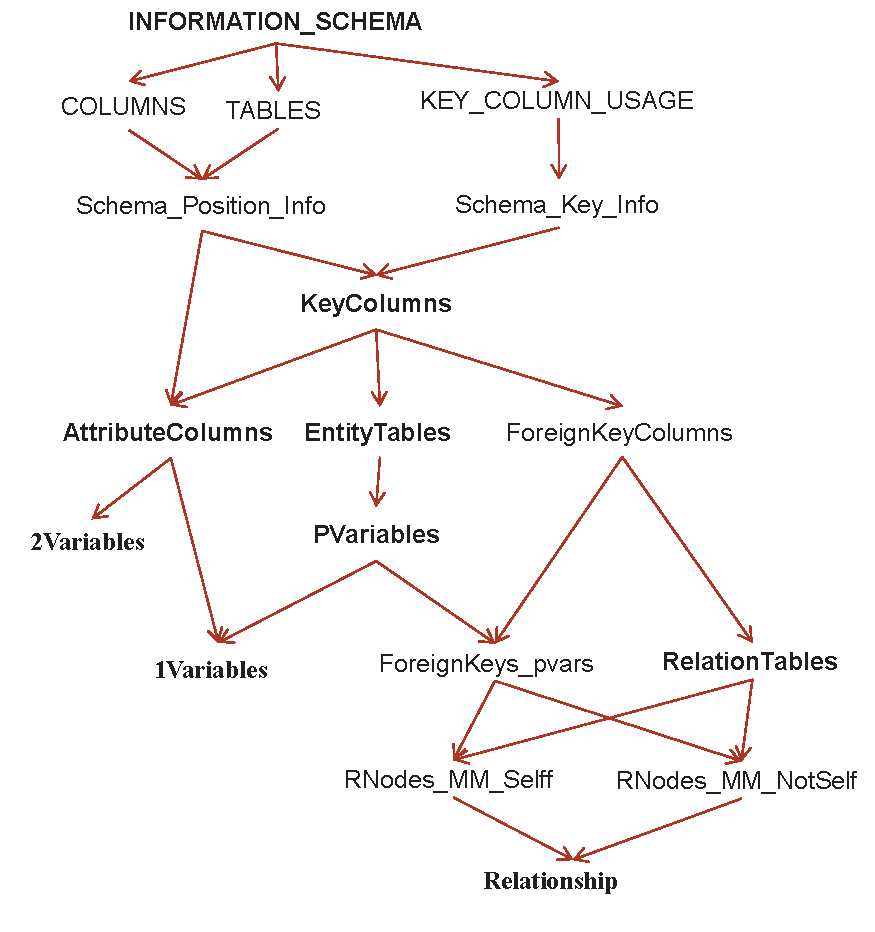
\includegraphics[width=0.5\textwidth]{rv_db.pdf} %move to the appendix
%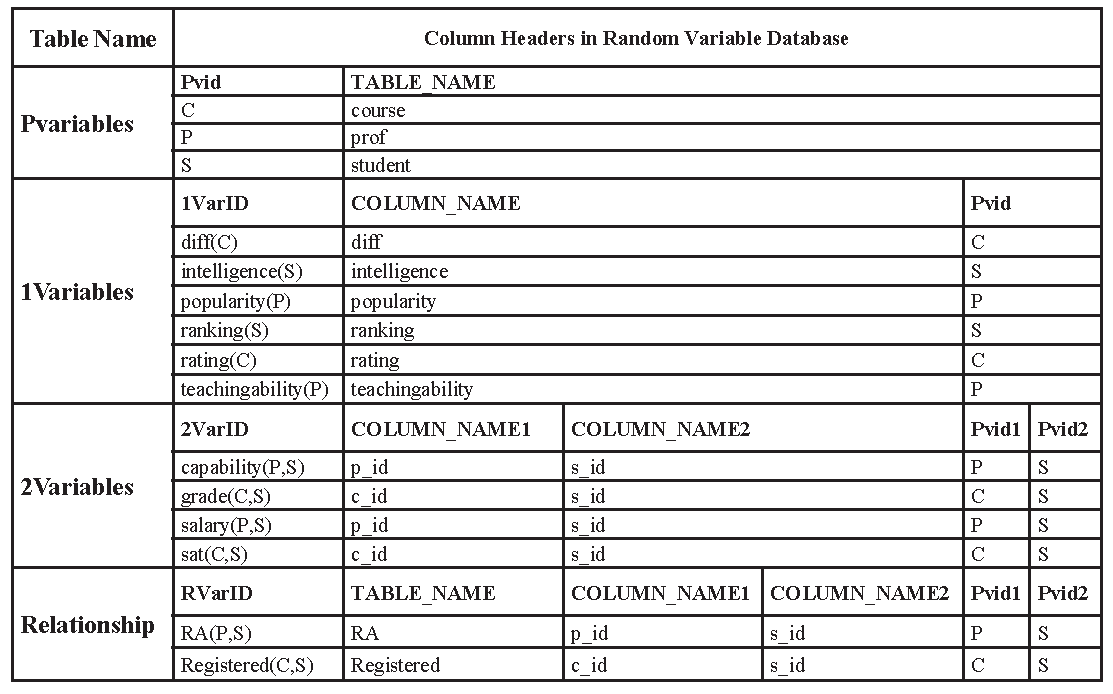
\includegraphics[width=0.5\textwidth]{rv_db_tables.pdf}
}
\caption{Tables  Dependency in the Random Variable Database $\RVD$.
\label{fig:rv_db1}}
\end{center}
\end{figure}

\section{MySQL Script for creating default random variables.}

\begin{scriptsize}
\begin{alltt}
/*AchemaAnalyzer.sql*/
DROP SCHEMA IF EXISTS @database@_AchemaAnalyzer; 
CREATE SCHEMA  @database@_AchemaAnalyzer;

CREATE SCHEMA  if not exists @database@_BN;
CREATE SCHEMA  if not exists @database@_CT;

USE @database@_AchemaAnalyzer;
SET storage_engine=INNODB;

CREATE TABLE Schema_Key_Info AS SELECT TABLE_NAME, COLUMN_NAME,
REFERENCED_TABLE_NAME, REFERENCED_COLUMN_NAME, CONSTRAINT_NAME FROM
INFORMATION_SCHEMA.KEY_COLUMN_USAGE WHERE (KEY_COLUMN_USAGE.TABLE_SCHEMA =
'@database@') ORDER BY TABLE_NAME;

CREATE TABLE Schema_Position_Info AS SELECT COLUMNS.TABLE_NAME,
COLUMNS.COLUMN_NAME,
COLUMNS.ORDINAL_POSITION FROM
INFORMATION_SCHEMA.COLUMNS,
INFORMATION_SCHEMA.TABLES
WHERE
(COLUMNS.TABLE_SCHEMA = '@database@'
    AND TABLES.TABLE_SCHEMA = '@database@'
    AND TABLES.TABLE_NAME = COLUMNS.TABLE_NAME
    AND TABLES.TABLE_TYPE = 'BASE TABLE')
ORDER BY TABLE_NAME;

CREATE TABLE NoPKeys AS SELECT TABLE_NAME FROM
Schema_Key_Info
WHERE
TABLE_NAME NOT IN (SELECT 
        TABLE_NAME
    FROM
        Schema_Key_Info
    WHERE
        CONSTRAINT_NAME LIKE 'PRIMARY');

CREATE table NumEntityColumns AS
SELECT 
    TABLE_NAME, COUNT(DISTINCT COLUMN_NAME) num
FROM
    Schema_Key_Info
WHERE
    CONSTRAINT_NAME LIKE 'PRIMARY'
        OR REFERENCED_COLUMN_NAME IS NOT NULL
GROUP BY TABLE_NAME;

CREATE TABLE TernaryRelations as SELECT TABLE_NAME FROM
NumEntityColumns
WHERE
num > 2;


CREATE TABLE AttributeColumns AS SELECT TABLE_NAME, COLUMN_NAME FROM
Schema_Position_Info
WHERE
(TABLE_NAME , COLUMN_NAME) NOT IN (SELECT 
        TABLE_NAME, COLUMN_NAME
    FROM
        KeyColumns)
    and TABLE_NAME NOT IN (SELECT 
        TABLE_NAME
    FROM
        NoPKeys)
    and TABLE_NAME NOT IN (SELECT 
        TABLE_NAME
    FROM
        TernaryRelations);

ALTER TABLE AttributeColumns ADD PRIMARY KEY (TABLE_NAME,COLUMN_NAME);

CREATE TABLE InputColumns AS SELECT * FROM
KeyColumns
WHERE
CONSTRAINT_NAME = 'PRIMARY'
ORDER BY TABLE_NAME;

CREATE TABLE ForeignKeyColumns AS SELECT * FROM
KeyColumns
WHERE
REFERENCED_COLUMN_NAME IS NOT NULL
ORDER BY TABLE_NAME;

ALTER TABLE ForeignKeyColumns ADD PRIMARY KEY (TABLE_NAME,COLUMN_NAME,
REFERENCED_TABLE_NAME);

CREATE TABLE EntityTables AS SELECT distinct TABLE_NAME, COLUMN_NAME 
FROM
KeyColumns T
WHERE
1 = (SELECT 
        COUNT(COLUMN_NAME)
    FROM
        KeyColumns T2
    WHERE
        T.TABLE_NAME = T2.TABLE_NAME
            AND CONSTRAINT_NAME = 'PRIMARY');

ALTER TABLE EntityTables ADD PRIMARY KEY (TABLE_NAME,COLUMN_NAME);

CREATE TABLE SelfRelationships AS SELECT DISTINCT RTables1.TABLE_NAME 
AS TABLE_NAME,
RTables1.REFERENCED_TABLE_NAME AS REFERENCED_TABLE_NAME,
RTables1.REFERENCED_COLUMN_NAME AS REFERENCED_COLUMN_NAME FROM
KeyColumns AS RTables1,
KeyColumns AS RTables2
WHERE
(RTables1.TABLE_NAME = RTables2.TABLE_NAME)
    AND (RTables1.REFERENCED_TABLE_NAME = RTables2.REFERENCED_TABLE_NAME)
    AND (RTables1.REFERENCED_COLUMN_NAME = RTables2.REFERENCED_COLUMN_NAME)
    AND (RTables1.ORDINAL_POSITION < RTables2.ORDINAL_POSITION);

ALTER TABLE SelfRelationships ADD PRIMARY KEY (TABLE_NAME);

CREATE TABLE Many_OneRelationships AS SELECT KeyColumns1.TABLE_NAME FROM
KeyColumns AS KeyColumns1,
KeyColumns AS KeyColumns2
WHERE
(KeyColumns1.TABLE_NAME , KeyColumns1.COLUMN_NAME) IN (SELECT 
        TABLE_NAME, COLUMN_NAME
    FROM
        InputColumns)
    AND (KeyColumns2.TABLE_NAME , KeyColumns2.COLUMN_NAME) IN (SELECT 
        TABLE_NAME, COLUMN_NAME
    FROM
        ForeignKeyColumns)
    AND (KeyColumns2.TABLE_NAME , KeyColumns2.COLUMN_NAME) NOT IN (SELECT 
        TABLE_NAME, COLUMN_NAME
    FROM
        InputColumns);

CREATE TABLE PVariables AS SELECT CONCAT(EntityTables.TABLE_NAME, '0') AS Pvid,
EntityTables.TABLE_NAME,
0 AS index_number FROM
EntityTables 
UNION 
SELECT 
CONCAT(EntityTables.TABLE_NAME, '1') AS Pvid,
EntityTables.TABLE_NAME,
1 AS index_number
FROM
EntityTables,
SelfRelationships
WHERE
EntityTables.TABLE_NAME = SelfRelationships.REFERENCED_TABLE_NAME
    AND EntityTables.COLUMN_NAME = SelfRelationships.REFERENCED_COLUMN_NAME ;

ALTER TABLE PVariables ADD PRIMARY KEY (Pvid);

CREATE TABLE RelationTables AS SELECT DISTINCT ForeignKeyColumns.TABLE_NAME,
ForeignKeyColumns.TABLE_NAME IN (SELECT 
        TABLE_NAME
    FROM
        SelfRelationships) AS SelfRelationship,
ForeignKeyColumns.TABLE_NAME IN (SELECT 
        TABLE_NAME
    FROM
        Many_OneRelationships) AS Many_OneRelationship FROM
ForeignKeyColumns;

ALTER TABLE RelationTables ADD PRIMARY KEY (TABLE_NAME);

CREATE TABLE 1Variables AS SELECT CONCAT('`', COLUMN_NAME, '(', Pvid, ')', '`') AS 1VarID,
COLUMN_NAME,
Pvid,
index_number = 0 AS main FROM
PVariables
    NATURAL JOIN
AttributeColumns;

ALTER TABLE 1Variables ADD PRIMARY KEY (1VarID);
ALTER TABLE 1Variables ADD UNIQUE(Pvid,COLUMN_NAME);

CREATE TABLE ForeignKeys_pvars AS SELECT ForeignKeyColumns.TABLE_NAME,
ForeignKeyColumns.REFERENCED_TABLE_NAME,
ForeignKeyColumns.COLUMN_NAME,
Pvid,
index_number,
ORDINAL_POSITION AS ARGUMENT_POSITION FROM
ForeignKeyColumns,
PVariables
WHERE
PVariables.TABLE_NAME = REFERENCED_TABLE_NAME;

ALTER TABLE ForeignKeys_pvars ADD PRIMARY KEY (TABLE_NAME,Pvid,
ARGUMENT_POSITION);

CREATE table Relationship_MM_NotSelf AS
SELECT 
    CONCAT('`',
            ForeignKeys_pvars1.TABLE_NAME,
            '(',
            ForeignKeys_pvars1.Pvid,
            ',',
            ForeignKeys_pvars2.Pvid,
            ')',
            '`') AS orig_RVarID,
    ForeignKeys_pvars1.TABLE_NAME,
    ForeignKeys_pvars1.Pvid AS Pvid1,
    ForeignKeys_pvars2.Pvid AS Pvid2,
    ForeignKeys_pvars1.COLUMN_NAME AS COLUMN_NAME1,
    ForeignKeys_pvars2.COLUMN_NAME AS COLUMN_NAME2,
    (ForeignKeys_pvars1.index_number = 0
        AND ForeignKeys_pvars2.index_number = 0) AS main
FROM
    ForeignKeys_pvars AS ForeignKeys_pvars1,
    ForeignKeys_pvars AS ForeignKeys_pvars2,
    RelationTables
WHERE
    ForeignKeys_pvars1.TABLE_NAME = ForeignKeys_pvars2.TABLE_NAME
        AND RelationTables.TABLE_NAME = ForeignKeys_pvars1.TABLE_NAME
        AND ForeignKeys_pvars1.ARGUMENT_POSITION <
        ForeignKeys_pvars2.ARGUMENT_POSITION
        AND RelationTables.SelfRelationship = 0
        AND RelationTables.Many_OneRelationship = 0;

CREATE table Relationship_MM_Self AS
SELECT 
    CONCAT('`',
            ForeignKeys_pvars1.TABLE_NAME,
            '(',
            ForeignKeys_pvars1.Pvid,
            ',',
            ForeignKeys_pvars2.Pvid,
            ')',
            '`') AS orig_RVarID,
    ForeignKeys_pvars1.TABLE_NAME,
    ForeignKeys_pvars1.Pvid AS Pvid1,
    ForeignKeys_pvars2.Pvid AS Pvid2,
    ForeignKeys_pvars1.COLUMN_NAME AS COLUMN_NAME1,
    ForeignKeys_pvars2.COLUMN_NAME AS COLUMN_NAME2,
    (ForeignKeys_pvars1.index_number = 0
        AND ForeignKeys_pvars2.index_number = 1) AS main
FROM
    ForeignKeys_pvars AS ForeignKeys_pvars1,
    ForeignKeys_pvars AS ForeignKeys_pvars2,
    RelationTables
WHERE
    ForeignKeys_pvars1.TABLE_NAME = ForeignKeys_pvars2.TABLE_NAME
        AND RelationTables.TABLE_NAME = ForeignKeys_pvars1.TABLE_NAME
        AND ForeignKeys_pvars1.ARGUMENT_POSITION <
        ForeignKeys_pvars2.ARGUMENT_POSITION
        AND ForeignKeys_pvars1.index_number < ForeignKeys_pvars2.index_number
        AND RelationTables.SelfRelationship = 1
        AND RelationTables.Many_OneRelationship = 0;

CREATE table Relationship_MO_NotSelf AS
SELECT 
    CONCAT('`',
            ForeignKeys_pvars.REFERENCED_TABLE_NAME,
            '(',
            PVariables.Pvid,
            ')=',
            ForeignKeys_pvars.Pvid,
            '`') AS orig_RVarID,
    ForeignKeys_pvars.TABLE_NAME,
    PVariables.Pvid AS Pvid1,
    ForeignKeys_pvars.Pvid AS Pvid2,
    KeyColumns.COLUMN_NAME AS COLUMN_NAME1,
    ForeignKeys_pvars.COLUMN_NAME AS COLUMN_NAME2,
    (PVariables.index_number = 0
        AND ForeignKeys_pvars.index_number = 0) AS main
FROM
    ForeignKeys_pvars,
    RelationTables,
    KeyColumns,
    PVariables
WHERE
    RelationTables.TABLE_NAME = ForeignKeys_pvars.TABLE_NAME
        AND RelationTables.TABLE_NAME = PVariables.TABLE_NAME
        AND RelationTables.TABLE_NAME = KeyColumns.TABLE_NAME
        AND RelationTables.SelfRelationship = 0
        AND RelationTables.Many_OneRelationship = 1;

CREATE table Relationship_MO_Self AS
SELECT 
    CONCAT('`',
            ForeignKeys_pvars.REFERENCED_TABLE_NAME,
            '(',
            PVariables.Pvid,
            ')=',
            ForeignKeys_pvars.Pvid,
            '`') AS orig_RVarID,
    ForeignKeys_pvars.TABLE_NAME,
    PVariables.Pvid AS Pvid1,
    ForeignKeys_pvars.Pvid AS Pvid2,
    KeyColumns.COLUMN_NAME AS COLUMN_NAME1,
    ForeignKeys_pvars.COLUMN_NAME AS COLUMN_NAME2,
    (PVariables.index_number = 0
        AND ForeignKeys_pvars.index_number = 1) AS main
FROM
    ForeignKeys_pvars,
    RelationTables,
    KeyColumns,
    PVariables
WHERE
    RelationTables.TABLE_NAME = ForeignKeys_pvars.TABLE_NAME
        AND RelationTables.TABLE_NAME = PVariables.TABLE_NAME
        AND RelationTables.TABLE_NAME = KeyColumns.TABLE_NAME
        AND PVariables.index_number < ForeignKeys_pvars.index_number
        AND RelationTables.SelfRelationship = 1
        AND RelationTables.Many_OneRelationship = 1;

CREATE TABLE Relationship AS SELECT * FROM  
Relationship_MM_NotSelf    
UNION SELECT            
*                   
FROM
Relationship_MM_Self 
UNION SELECT 
*
FROM
Relationship_MO_NotSelf 
UNION SELECT 
*
FROM
Relationship_MO_Self;

ALTER TABLE Relationship ADD PRIMARY KEY (orig_RVarID);
ALTER TABLE `Relationship` ADD COLUMN `RVarID` VARCHAR(10) NULL , 
ADD UNIQUE INDEX `RVarID_UNIQUE` (`RVarID` ASC) ; 


CREATE TABLE 2Variables AS SELECT CONCAT('`',
        COLUMN_NAME,
        '(',
        Pvid1,
        ',',
        Pvid2,
        ')',
        '`') AS 2VarID,
COLUMN_NAME,
Pvid1,
Pvid2,
TABLE_NAME,
main FROM
Relationship
    NATURAL JOIN
AttributeColumns;

ALTER TABLE 2Variables ADD PRIMARY KEY (2VarID);</p>\end{alltt}

%\section{Final Thoughts on Good Layout}
%Please use readable font sizes in the figures and graphs. Avoid tempering with the correct border values, and the spacing (and format) of both text and captions of the PVLDB format (e.g. captions are bold).
%
%At the end, please check for an overall pleasant layout, e.g. by ensuring a readable and logical positioning of any floating figures and tables. Please also check for any line overflows, which are only allowed in extraordinary circumstances (such as wide formulas or URLs where a line wrap would be counterintuitive).
%
%Use the \texttt{balance} package together with a \texttt{\char'134 balance} command at the end of your document to ensure that the last page has balanced (i.e. same length) columns.
\end{scriptsize}



\end{appendix}

%ACKNOWLEDGMENTS are optional
%\section{Acknowledgments}
%
%This research was supported by a Discovery grant to Oliver Schulte by the Natural Sciences and Engineering Research Council of Canada. 
%Zhensong Qian was supported by a grant from the China Scholarship Council.
%We thank the organizers for providing a discussion venue, and the anonymous reviewers for constructive criticism.




 % vldb_sample.bib is the name of the Bibliography in this case
% You must have a proper ".bib" file
%  and remember to run:
% latex bibtex latex latex
% to resolve all references

%\subsection{References}

%%APPENDIX is optional.
%% ****************** APPENDIX **************************************
%% Example of an appendix; typically would start on a new page
%\newpage
%\pagebreak
%



\end{document}


